\documentclass[oribibl]{llncs}

\usepackage{booktabs} % For formal tables

%%%%%%%%%%%%%%%%%%%%%%%%%%%%%%%%%%%%%%%%%%%%%%%%%%%%%%%%%%%%%%%%%%%%%%%%%%%%%%%%%
%%%%%%%%%%%%%%%%%%%%%%%%%%%%%%% customize begin %%%%%%%%%%%%%%%%%%%%%%%%%%%%%%%%
% \usepackage{appendix}
\usepackage{amsfonts}
\usepackage{enumerate,paralist}
\usepackage{mathtools}
\usepackage{amsmath}
\usepackage{stmaryrd}

\usepackage{tikz,pgffor}
\usetikzlibrary{arrows}
\usetikzlibrary{shapes}
\usetikzlibrary{calc}
\usetikzlibrary{automata}
\usetikzlibrary{positioning}

\tikzstyle{location} = [
    rectangle,
    rounded corners,
    draw=black,
    very thick,
    minimum height=2em,
    inner sep=0pt,
    text centered
]
\tikzstyle{tran}  = [
    draw,
    ->,
    >=stealth,
    rounded corners
]
\tikzstyle{nchoice}  = [
    draw,
    >=stealth,
    rounded corners
]
\tikzstyle{pchoice}  = [
    draw,
    ->,
    >=stealth,
    rounded corners,
    dashed
]
\tikzstyle{dec}   = [inner sep=0pt]
\tikzstyle{mode}  = [
    shape=circle,
    draw,
    inner sep=0pt,
    minimum size=5mm
]

%\theoremstyle{plain}
%\newtheorem{lemma}{Lemma}
%\newtheorem{claim}{Claim}
%\newtheorem{proposition}{Proposition}
%\newtheorem{definition}{Definition}
%\newtheorem{corollary}{Corollary}
%\newtheorem{theorem}{Theorem}
%\newtheorem{example}{Example}
%\newtheorem{remark}{Remark}
%\newtheorem{observation}{Observation}
%\newtheorem{assumption}{Assumption}

%% Notations

%%General Notations

\newcommand{\Rset}{\mathbb{R}}
\newcommand{\Nset}{\mathbb{N}}
\newcommand{\Zset}{\mathbb{Z}}
\newcommand{\ap}{\mbox{\sl AP}}
\newcommand{\opt}{\mbox{\sl opt}}

%%Clocks and Clock Constraints

\newcommand{\clocks}{\mathcal{X}}
\newcommand{\val}[1]{\mbox{\sl Val}\left(#1\right)}
\newcommand{\reset}[2]{{#1}{\left[#2:=0\right]}}
\newcommand{\add}[2]{{#1}{+}{#2}}
\newcommand{\zero}{\mathbf{0}}
\newcommand{\true}{\mathbf{true}}
\newcommand{\false}{\mathbf{false}}
\newcommand{\supp}[1]{{\mbox{\sl supp}}(#1)}
\newcommand{\dist}[1]{{\mathcal{D}}{\left(#1\right)}}
\newcommand{\sat}[1]{{\llbracket}{#1}{\rrbracket}}
\newcommand{\intp}[1]{{\lfloor}{#1}{\rfloor}}
\newcommand{\fracp}[1]{\mbox{\sl frac}(#1)}
\newcommand{\evclass}[1]{\left[#1\right]}

%%PTAs

\newcommand{\pta}{\mathcal{C}}
\newcommand{\locs}{L}
\newcommand{\loc}{\ell}
\newcommand{\acts}{\mbox{\sl Act}}
\newcommand{\inv}{\mbox{\sl inv}}
\newcommand{\enab}{\mbox{\sl enab}}
\newcommand{\penab}[2]{\mbox{\sl enab}\left(
    {#1},{#2}
\right ) }
\newcommand{\prob}{\mbox{\sl prob}}
\newcommand{\lbfunc}{\mathcal{L}}
\newcommand{\clcons}[1]{\mbox{\sl CC}\left(#1\right)}
\newcommand{\istate}{\left(\loc^*,\mathbf{0}\right)}

%% Semantics of PTAs

\newcommand{\states}{S}
\newcommand{\trans}{\rightarrow}
\newcommand{\tran}[3]{{#1}{\xrightarrow{#2}}{#3}}
\newcommand{\probk}{\mathbf{P}}

\newcommand{\fnpaths }[1]{\mbox{\sl Paths}^*_{#1}}
\newcommand{\infpaths}[1]{\mbox{\sl Paths}^\omega_{#1}}
\newcommand{\omgpaths}[2]{\mbox{\sl Reach}^{#2}_{#1}}
\newcommand{\initloc }[1]{\mbox{\sl init}\left(#1\right)}
\newcommand{\lastloc }[1]{\mbox{\sl last}\left(#1\right)}

\newcommand{\fnpath}{\rho}
\newcommand{\infpath}{\pi}

\newcommand{\length}[1]{\left| #1 \right|}

%% Notations for Probability Space

\newcommand{\probm}{\mathbb{P}}
\newcommand{\expv}{\mathbb{E}}
\newcommand{\cyl}{\mbox{\sl Cyl}}

%% Notations for DTAs

\newcommand{\dta}{\mathcal{A}}
\newcommand{\dtloc}{q}
\newcommand{\dtclocks}{\mathcal{Y}}
\newcommand{\cstates}{Q}
\newcommand{\alphabet}{\Sigma}
\newcommand{\rules}{\Delta}
\newcommand{\dtphi}[3]{\Phi_{#1,#2}^{#3}}
\newcommand{\dtx}[3]{\mathbf{X}_{#1,#2}^{#3}}
\newcommand{\dtq}[3]{\mathbf{q}_{#1,#2}^{#3}}
\newcommand{\trfunc}{\kappa}
\newcommand{\dtatr}[3]{{#1}{\xRightarrow{#2}}{#3}}
\newcommand{\regions}{\mathcal{G}}

\newcommand{\run}[3]{{#1}_{#2}\left(#3\right)}
\newcommand{\iconfig}{\left(\dtloc^*,\mathbf{0}\right)}

%%Product Constrution
\newcommand{\product}[2]{{#1}{\otimes}{#2}}
\newcommand{\pr}[2]{\mathfrak{p}_{#1}^{#2}}
\newcommand{\pfunc}{\mathcal{T}}
\newcommand{\sfunc}{\theta}
\newcommand{\acc}[2]{{\mbox{\sl AccPaths}}_{#1}^{#2}}
\newcommand{\extactions}{\mathcal{B}}
\newcommand{\exttuples}{\mathcal{T}}

%%Reward Structure
\newcommand{\rcum}{\mathbf{r}_{\locs}}
\newcommand{\rinst}{\mathbf{r}_{\acts}}
\newcommand{\ronestep}{\mathbf{r}}
\newcommand{\accum}[1]{\mbox{\sl Cum}_{#1}}
\newcommand{\rd}[2]{\mathsf{R}_{#1}^{#2}}

%%Rabin acceptance

% \newcommand{\infset}[1]{\mbox{\sl{inf  }} ( #1 )}
% \newcommand{\trace }[1]{\mbox{\sl{trace}} ( #1 )}
% \newcommand{\traj  }[1]{\mbox{\sl{traj }} ( #1 )}
\newcommand{\infset}[1]{\mbox{\sl inf}  ( #1 )}
\newcommand{\trace }[1]{\mbox{\sl trace}( #1 )}
\newcommand{\traj  }[1]{\mbox{\sl traj} ( #1 )}
\newcommand{\rabin}{\mathcal{F}}

%%Finite acceptance
\newcommand{\fstates}{F}

\newcommand{\Lang}[2] {
    \mbox{\sl AccPaths}
        _{#1}
        ^{#2}
}

\newcommand{\rabinp}[1]{\mbox{\sl RPaths}_{#1}}

\newcommand{\Accept}[1]{
    \mbox{\sl RabinPaths}
        _{#1}
        % ^{#2}
}

\newcommand{\LangCsAqF}{
    \Lang
        {\pta,\sigma}
        {\dta,\dtloc}
}

\newcommand{\AcceptCxAqsF}{
    \Accept
        {
            \product{\pta}{\dta_\dtloc},
            \sigma
        }
        % {\rabin}
}

\newcommand{\TLang}{
    \pfunc\left(
        \LangCsAqF
    \right)
}

\newcommand{\TAcc}{
%    \Accept
%        {
%            \product{\pta}{\dta_\dtloc},
%            \sfunc \left(
%                \sigma
%            \right)
%        }
    \rabinp{\sfunc\left(\sigma\right)}
        % {\rabin}
}
\newcommand{\accept}[2]{
    \mbox{\bf ACC} \left(
      {#1},
      {#2}
    \right)
}
\newcommand{\acccept}[3]{
    \mbox{\bf ACC} \left(
      {#1},
      {#2},
      {#3}
    \right)
}
\newcommand{\accccept}[4]{
    \mbox{\bf ACC} \left(
      {#1},
      {#2},
      {#3},
      {#4}
    \right)
}
%% Proudct
\newcommand{\Region}[1]{
  \mbox{Reg}[
    {#1}
  ]
}
\newcommand{\WAIT}[0]{\mbox{\sl WAIT}}
\newcommand{\WORK}[1]{\mbox{\sl WORK}_{#1}}
\newcommand{\DONE}[1]{\mbox{\sl DONE}_{#1}}
\newcommand{\request}[1]{\mbox{\sl Req}_{#1}}
\newcommand{\p}[1]{\mbox{\sl p}_{#1}}

\def\INIT{  \mbox{\sl INIT} }
\def\FAIL{  \mbox{\sl FAIL} }
\newcommand{\q}[1]{\mbox{\sl q}_{#1}}

\newcommand{\location}[5]{
    \node[location] (#1) at #2 {
        \begin{tabular}{c}
            \ensuremath{#3} \\
            \hline
            \ensuremath{#4} \\
            \ensuremath{#5}
        \end{tabular}
    }
}

\newcommand{\PairV}[2]{#1#2}
\newcommand{\PairS}[2]{({#1},{#2})}

%%For drawing grids

\newcounter{row}
\newcounter{col}

\newcommand\setrow[3]{
  \setcounter{col}{1}
  \foreach \n in {#1, #2, #3} {
    \edef\x{\value{col} - 0.5}
    \edef\y{3.5 - \value{row}}
    \node[anchor=center] at (\x, \y) {\n};
    \stepcounter{col}
  }
  \stepcounter{row}
}

% Undecidability
\newcommand{\nta}{\mathcal{A}}
\newcommand{\qinit}{q_{\mbox{\sl\scriptsize init} }}
\newcommand{\qstart}{q_{\mbox{\sl\scriptsize start}}}
\newcommand{\ntaap}[1]{b_{#1}}
\newcommand{\PCswLang}{
    \probm^{\pta,\sigma_w }\left(
    \Lang
        {\pta,\sigma_w}
        {\nta',\qinit,\rabin}
    \right)
}

\newcommand{\TRA}{TRA}
\newcommand{\tra}{\mathcal{A}}

% INF MDP
\newcommand{\clocksX}{\mathcal{X}}
\newcommand{\clocksY}{\mathcal{Y}}
\newcommand{\reg}{R}
\newcommand{\floor}[1]{\mbox{\sl floor} \left (
    {#1}
\right )}
\newcommand{\productmdp}[2]{{#1}{\ast}{#2}}
\newcommand{\mdploc}{s}
\newcommand{\project}[2]{
    {#1} \downarrow {#2}
}
\newcommand{\pair}[2]{
    \left (
        {#1}
        ,
        {#2}
    \right )
}
\newcommand{\clocksALL}{
    \clocksX \cup \left(
        \bigcup_{k=1}^{n} \clocksY_k
    \right )
}
%%%%%%%%%%%%%%%%%%%%%%%%%%%%%% customize end %%%%%%%%%%%%%%%%%%%%%%%%%%%%%%
%%%%%%%%%%%%%%%%%%%%%%%%%%%%%%%%%%%%%%%%%%%%%%%%%%%%%%%%%%%%%%%%%%%%%%%%%%%

% Copyright
% \setcopyright{none}
%\setcopyright{acmcopyright}
%\setcopyright{acmlicensed}
%%%%%% \setcopyright{rightsretained}
%\setcopyright{usgov}
%\setcopyright{usgovmixed}
%\setcopyright{cagov}
%\setcopyright{cagovmixed}


% DOI
% \acmDOI{10.475/123_4}

% ISBN
% \acmISBN{123-4567-24-567/08/06}

%Conference
%\acmConference[HSCC 2018]{ACM International Conference on Hybrid Systems: Computation and Control }{April 2018}{
%  Porto, Portugal
%}
% \acmConference{HSCC 2018}{April 2018}{
%   Porto, Portugal
% }
% \acmYear{1997}
% \copyrightyear{2017}

% \acmPrice{15.00}


\begin{document}
\title{Verifying Probabilistic Timed Automata Against \\Omega-Regular Dense-Time Properties}
% \subtitle{Verifying PTAs Against Timed-Automata Specifications}
% \titlenote{Produces the permission block, and
%   copyright information}
% \subtitlenote{The full version of the author's guide is available as
%   \texttt{acmart.pdf} document}

\author{
    Hongfei Fu\inst{1} 
    \and 
    Yi Li\inst{2} 
    \and 
    Jianlin Li\inst{3,4}
    % \and
    % Lijun Zhang\inst{4}
}
\institute{
    Shanghai Jiao Tong University, Shanghai, China
    % ,\\ \email{fuhf@cs.sjtu.edu.cn}
    \and
    Department of Informatics, School of Mathematical Sciences, Peking University, Beijing, China 
    % \\ \email{liyi\_math@pku.edu.cn}
    \and
    State Key Laboratory of Computer Science, Institute of Software, Chinese Academy of Sciences, Beijing, China
    \and
    College of Computer Science and Technology, Nanjing University of Aeronautics and Astronautics, Nanjing, China
    % \email{ljlin@nuaa.edu.cn}
    % State Key Laboratory of Computer Science, Institute of Software, Chinese Academy of Sciences, Beijing, China \\
    % \email{zhanglj@ios.ac.cn}
}

% \author{Hongfei Fu}
% % \authornote{Dr.~Trovato insisted his name be first.}
% % \orcid{1234-5678-9012}
% \affiliation{%
%   \institution{Shanghai Jiao Tong University}
%   % \streetaddress{P.O. Box 1212}
%   % \city{Shanghai}
%   % \state{China}
%   % \postcode{43017-6221}
% }
% \email{fuhf@ios.ac.cn}

% \author{Yi Li}
% % \authornote{The secretary disavows any knowledge of this author's actions.}
% \affiliation{%
%   \institution{Department of Informatics, School of Mathematical Sciences, Peking University}
%   % \streetaddress{P.O. Box 1212}
%   % \city{Beijing}
%   % \state{China}
%   % \postcode{43017-6221}
% }
% \email{liyi_math@pku.edu.cn}

% \author{Jianlin Li}
% \affiliation{%
%   \institution{College of Computer Science and Technology Nanjing University of Aeronautics and Astronautics}
%   % \streetaddress{P.O. Box 1212}
%   % \city{Beijing}
%   % \state{China}
%   % \postcode{43017-6221}
% }
% \email{ljlin@nuaa.edu.cn}

% \author{Lijun Zhang}
% \affiliation{%
%   \institution{State Key Laboratory of Computer Science, Institute of Software, Chinese Academy of Sciences}
%   % \streetaddress{P.O. Box 1212}
%   % \city{Beijing}
%   % \state{China}
%   % \postcode{43017-6221}
% }
% \email{zhanglj@ios.ac.cn}

% \author{Aparna Patel}
% \affiliation{%
%  \institution{Rajiv Gandhi University}
%  \streetaddress{Rono-Hills}
%  \city{Doimukh}
%  \state{Arunachal Pradesh}
%  \country{India}}
% \author{Huifen Chan}
% \affiliation{%
%   \institution{Tsinghua University}
%   \streetaddress{30 Shuangqing Rd}
%   \city{Haidian Qu}
%   \state{Beijing Shi}
%   \country{China}
% }

% The default list of authors is too long for headers}
% \renewcommand{\shortauthors}{B. Trovato et al.}

% \begin{comment}
% % \begin{abstract}
% % This paper provides a sample of a \LaTeX\ document which conforms,
% % somewhat loosely, to the formatting guidelines for
% % ACM SIG Proceedings.\footnote{This is an abstract footnote}
% % \end{abstract}

% %
% % The code below should be generated by the tool at
% % http://dl.acm.org/ccs.cfm
% % Please copy and paste the code instead of the example below.
% %
% \begin{CCSXML}
% <ccs2012>
%  <concept>
%   <concept_id>10010520.10010553.10010562</concept_id>
%   <concept_desc>Computer systems organization~Embedded systems</concept_desc>
%   <concept_significance>500</concept_significance>
%  </concept>
%  <concept>
%   <concept_id>10010520.10010575.10010755</concept_id>
%   <concept_desc>Computer systems organization~Redundancy</concept_desc>
%   <concept_significance>300</concept_significance>
%  </concept>
%  <concept>
%   <concept_id>10010520.10010553.10010554</concept_id>
%   <concept_desc>Computer systems organization~Robotics</concept_desc>
%   <concept_significance>100</concept_significance>
%  </concept>
%  <concept>
%   <concept_id>10003033.10003083.10003095</concept_id>
%   <concept_desc>Networks~Network reliability</concept_desc>
%   <concept_significance>100</concept_significance>
%  </concept>
% </ccs2012>
% \end{CCSXML}

% \ccsdesc[500]{Computer systems organization~Embedded systems}
% \ccsdesc[300]{Computer systems organization~Redundancy}
% \ccsdesc{Computer systems organization~Robotics}
% \ccsdesc[100]{Networks~Network reliability}


% \keywords{ACM proceedings, \LaTeX, text tagging}
% \end{comment}

\maketitle

\vspace{-2em}

  In this paper, we explore the connection between secret key agreement and secure omniscience within the setting of the multiterminal source model with a wiretapper who has side information. While the secret key agreement problem considers the generation of a maximum-rate secret key through public discussion, the secure omniscience problem is concerned with communication protocols for omniscience that minimize the rate of information leakage to the wiretapper. The starting point of our work is a lower bound on the minimum leakage rate for omniscience, $\rl$, in terms of the wiretap secret key capacity, $\wskc$. Our interest is in identifying broad classes of sources for which this lower bound is met with equality, in which case we say that there is a duality between secure omniscience and secret key agreement. We show that this duality holds in the case of certain finite linear source (FLS) models, such as two-terminal FLS models and pairwise independent network models on trees with a linear wiretapper. Duality also holds for any FLS model in which $\wskc$ is achieved by a perfect linear secret key agreement scheme. We conjecture that the duality in fact holds unconditionally for any FLS model. On the negative side, we give an example of a (non-FLS) source model for which duality does not hold if we limit ourselves to communication-for-omniscience protocols with at most two (interactive) communications.  We also address the secure function computation problem and explore the connection between the minimum leakage rate for computing a function and the wiretap secret key capacity.
  
%   Finally, we demonstrate the usefulness of our lower bound on $\rl$ by using it to derive equivalent conditions for the positivity of $\wskc$ in the multiterminal model. This extends a recent result of Gohari, G\"{u}nl\"{u} and Kramer (2020) obtained for the two-user setting.
  
   
%   In this paper, we study the problem of secret key generation through an omniscience achieving communication that minimizes the 
%   leakage rate to a wiretapper who has side information in the setting of multiterminal source model.  We explore this problem by deriving a lower bound on the wiretap secret key capacity $\wskc$ in terms of the minimum leakage rate for omniscience, $\rl$. 
%   %The former quantity is defined to be the maximum secret key rate achievable, and the latter one is defined as the minimum possible leakage rate about the source through an omniscience scheme to a wiretapper. 
%   The main focus of our work is the characterization of the sources for which the lower bound holds with equality \textemdash it is referred to as a duality between secure omniscience and wiretap secret key agreement. For general source models, we show that duality need not hold if we limit to the communication protocols with at most two (interactive) communications. In the case when there is no restriction on the number of communications, whether the duality holds or not is still unknown. However, we resolve this question affirmatively for two-user finite linear sources (FLS) and pairwise independent networks (PIN) defined on trees, a subclass of FLS. Moreover, for these sources, we give a single-letter expression for $\wskc$. Furthermore, in the direction of proving the conjecture that duality holds for all FLS, we show that if $\wskc$ is achieved by a \emph{perfect} secret key agreement scheme for FLS then the duality must hold. All these results mount up the evidence in favor of the conjecture on FLS. Moreover, we demonstrate the usefulness of our lower bound on $\wskc$ in terms of $\rl$ by deriving some equivalent conditions on the positivity of secret key capacity for multiterminal source model. Our result indeed extends the work of Gohari, G\"{u}nl\"{u} and Kramer in two-user case.

\vspace{-1em}

% \leavevmode
% \\
% \\
% \\
% \\
% \\
\section{Introduction}
\label{introduction}

AutoML is the process by which machine learning models are built automatically for a new dataset. Given a dataset, AutoML systems perform a search over valid data transformations and learners, along with hyper-parameter optimization for each learner~\cite{VolcanoML}. Choosing the transformations and learners over which to search is our focus.
A significant number of systems mine from prior runs of pipelines over a set of datasets to choose transformers and learners that are effective with different types of datasets (e.g. \cite{NEURIPS2018_b59a51a3}, \cite{10.14778/3415478.3415542}, \cite{autosklearn}). Thus, they build a database by actually running different pipelines with a diverse set of datasets to estimate the accuracy of potential pipelines. Hence, they can be used to effectively reduce the search space. A new dataset, based on a set of features (meta-features) is then matched to this database to find the most plausible candidates for both learner selection and hyper-parameter tuning. This process of choosing starting points in the search space is called meta-learning for the cold start problem.  

Other meta-learning approaches include mining existing data science code and their associated datasets to learn from human expertise. The AL~\cite{al} system mined existing Kaggle notebooks using dynamic analysis, i.e., actually running the scripts, and showed that such a system has promise.  However, this meta-learning approach does not scale because it is onerous to execute a large number of pipeline scripts on datasets, preprocessing datasets is never trivial, and older scripts cease to run at all as software evolves. It is not surprising that AL therefore performed dynamic analysis on just nine datasets.

Our system, {\sysname}, provides a scalable meta-learning approach to leverage human expertise, using static analysis to mine pipelines from large repositories of scripts. Static analysis has the advantage of scaling to thousands or millions of scripts \cite{graph4code} easily, but lacks the performance data gathered by dynamic analysis. The {\sysname} meta-learning approach guides the learning process by a scalable dataset similarity search, based on dataset embeddings, to find the most similar datasets and the semantics of ML pipelines applied on them.  Many existing systems, such as Auto-Sklearn \cite{autosklearn} and AL \cite{al}, compute a set of meta-features for each dataset. We developed a deep neural network model to generate embeddings at the granularity of a dataset, e.g., a table or CSV file, to capture similarity at the level of an entire dataset rather than relying on a set of meta-features.
 
Because we use static analysis to capture the semantics of the meta-learning process, we have no mechanism to choose the \textbf{best} pipeline from many seen pipelines, unlike the dynamic execution case where one can rely on runtime to choose the best performing pipeline.  Observing that pipelines are basically workflow graphs, we use graph generator neural models to succinctly capture the statically-observed pipelines for a single dataset. In {\sysname}, we formulate learner selection as a graph generation problem to predict optimized pipelines based on pipelines seen in actual notebooks.

%. This formulation enables {\sysname} for effective pruning of the AutoML search space to predict optimized pipelines based on pipelines seen in actual notebooks.}
%We note that increasingly, state-of-the-art performance in AutoML systems is being generated by more complex pipelines such as Directed Acyclic Graphs (DAGs) \cite{piper} rather than the linear pipelines used in earlier systems.  
 
{\sysname} does learner and transformation selection, and hence is a component of an AutoML systems. To evaluate this component, we integrated it into two existing AutoML systems, FLAML \cite{flaml} and Auto-Sklearn \cite{autosklearn}.  
% We evaluate each system with and without {\sysname}.  
We chose FLAML because it does not yet have any meta-learning component for the cold start problem and instead allows user selection of learners and transformers. The authors of FLAML explicitly pointed to the fact that FLAML might benefit from a meta-learning component and pointed to it as a possibility for future work. For FLAML, if mining historical pipelines provides an advantage, we should improve its performance. We also picked Auto-Sklearn as it does have a learner selection component based on meta-features, as described earlier~\cite{autosklearn2}. For Auto-Sklearn, we should at least match performance if our static mining of pipelines can match their extensive database. For context, we also compared {\sysname} with the recent VolcanoML~\cite{VolcanoML}, which provides an efficient decomposition and execution strategy for the AutoML search space. In contrast, {\sysname} prunes the search space using our meta-learning model to perform hyperparameter optimization only for the most promising candidates. 

The contributions of this paper are the following:
\begin{itemize}
    \item Section ~\ref{sec:mining} defines a scalable meta-learning approach based on representation learning of mined ML pipeline semantics and datasets for over 100 datasets and ~11K Python scripts.  
    \newline
    \item Sections~\ref{sec:kgpipGen} formulates AutoML pipeline generation as a graph generation problem. {\sysname} predicts efficiently an optimized ML pipeline for an unseen dataset based on our meta-learning model.  To the best of our knowledge, {\sysname} is the first approach to formulate  AutoML pipeline generation in such a way.
    \newline
    \item Section~\ref{sec:eval} presents a comprehensive evaluation using a large collection of 121 datasets from major AutoML benchmarks and Kaggle. Our experimental results show that {\sysname} outperforms all existing AutoML systems and achieves state-of-the-art results on the majority of these datasets. {\sysname} significantly improves the performance of both FLAML and Auto-Sklearn in classification and regression tasks. We also outperformed AL in 75 out of 77 datasets and VolcanoML in 75  out of 121 datasets, including 44 datasets used only by VolcanoML~\cite{VolcanoML}.  On average, {\sysname} achieves scores that are statistically better than the means of all other systems. 
\end{itemize}


%This approach does not need to apply cleaning or transformation methods to handle different variances among datasets. Moreover, we do not need to deal with complex analysis, such as dynamic code analysis. Thus, our approach proved to be scalable, as discussed in Sections~\ref{sec:mining}.
%!TEX root = hopfwright.tex
%

In this section we systematically recast the Hopf bifurcation problem in Fourier space. 
We introduce appropriate scalings, sequence spaces of Fourier coefficients and convenient operators on these spaces. 
To study Equation~\eqref{eq:FourierSequenceEquation} we consider Fourier sequences $ \{a_k\}$ and fix a Banach space in which these sequences reside. It is indispensable for our analysis that this space have an algebraic structure. 
The Wiener algebra of absolutely summable Fourier series is a natural candidate, which we use with minor modifications. 
In numerical applications, weighted sequence spaces with algebraic and geometric decay have been used to great effect to study periodic solutions which are $C^k$ and analytic, respectively~\cite{lessard2010recent,hungria2016rigorous}. 
Although it follows from Lemma~\ref{l:analytic} that the Fourier coefficients of any solution decay exponentially, we choose to work in a space of less regularity. 
The reason is that by working in a space with less regularity, we are better able to connect our results with the global estimates in \cite{neumaier2014global}, see Theorem~\ref{thm:UniqunessNbd2}.


%
%
%\begin{remark}
%	Although it follows from Lemma~\ref{l:analytic} that the Fourier coefficients of any solution decay exponentially, we choose to work in a space of less regularity, namely summable Fourier coefficients. This allows us to draw SOME MORE INTERESTING CONCLUSION LATER.
%	EXPLAIN WHY WE CHOOSE A NORM WITH ALMOST NO DECAY!
%	% of s Periodic solutions to Wright's equation are known to be real analytic and so their  Fourier coefficients must decay geometrically [Nussbaum].
%	% We do not use such a strong result;  any periodic solution must be continuously differentiable, by which it follows that $ \sum | c_k| < \infty$.
%\end{remark}


\begin{remark}\label{r:a0}
There is considerable redundancy in Equation~\eqref{eq:FourierSequenceEquation}. First, since we are considering real-valued solutions $y$, we assume $\c_{-k}$ is the complex conjugate of $\c_k$. This symmetry implies it suffices to consider Equation~\eqref{eq:FourierSequenceEquation} for $k \geq 0$.
Second, we may effectively ignore the zeroth Fourier coefficient of any periodic solution \cite{jones1962existence}, since it is necessarily equal to $0$. 
%In \cite{jones1962existence}, it is shown that if $y \not\equiv -1$ is a periodic solution of~\eqref{eq:Wright} with frequency $\omega$, then $ \int_0^{2\pi/\omega} y(t) dt =0$. 
		The self contained argument is as follows. 
		As mentioned in the introduction, any periodic solution to Wright's equation must satisfy $ y(t) > -1$ for all $t$. 
	By dividing Equation~\eqref{eq:Wright} by $(1+y(t))$, which never vanishes, we obtain
	\[
	\frac{d}{dt} \log (1 + y(t)) = - \alpha y(t-1).
	\]  
	Integrating over one period $L$ we derive the condition 
	$0=\int_0^L y(t) dt $.
	Hence $a_0=0$ for any periodic solution. 
	It will be shown in Theorem~\ref{thm:FourierEquivalence1} that a related argument implies that we do not need to consider Equation~\eqref{eq:FourierSequenceEquation} for $k=0$.
\end{remark}

%%%
%%%
%%%\begin{remark}\label{r:c0} 
%%%In \cite{jones1962existence}, it is shown that if $y \not\equiv -1$ is a periodic solution of~\eqref{eq:Wright} with frequency $\omega$, then $ \int_0^{2\pi/\omega} y(t) dt =0$. 
%%%PERHAPS TOO MUCH DETAIL HERE. The self contained argument is as follows.
%%%If $y \not\equiv -1$ then $y(t) \neq -1$ for all $t$, since if $y(t_0)=-1$ for some $t_0 \in \R$ then $y'(t_0)=0$ by~\eqref{eq:Wright} and in fact by differentiating~\eqref{eq:Wright} repeatedly one obtains that all derivatives of $y$ vanish at $t_0$. Hence $y \equiv -1$ by Lemma~\ref{l:analytic}, a contradiction. Now divide~\eqref{eq:Wright} by $(1+y(t))$, which never vanishes, to obtain
%%%\[
%%%  \frac{d}{dt} \log |1 + y(t)| = - \alpha y(t-1).
%%%\]  
%%%Integrating over one period we obtain $\int_0^L y(t) dt =0$.
%%%\end{remark}



%Furthermore, the condition that $y(t)$ is real forces $\c_{-k} = \overline{\c}_{k}$.  
%
We define the spaces of absolutely summable Fourier series
\begin{alignat*}{1}
	\ell^1 &:= \left\{ \{ \c_k \}_{k \geq 1} : 
    \sum_{k \geq 1} | \c_k| < \infty  \right\} , \\
	\ell^1_\bi &:= \left\{ \{ \c_k \}_{k \in \Z} : 
    \sum_{k \in \Z} | \c_k| < \infty  \right\} .
\end{alignat*} 
We identify any semi-infinite sequence $ \{ \c_k \}_{k \geq 1} \in \ell^1$ with the bi-infinite sequence $ \{ \c_k \}_{k \in \Z} \in \ell^1_\bi$ via the conventions (see Remark~\ref{r:a0})
\begin{equation}
  \c_0=0 \qquad\text{ and }\qquad \c_{-k} = \c_{k}^*. 
\end{equation}
In other word, we identify $\ell^1$ with the set
\begin{equation*}
   \ell^1_\sym := \left\{ \c \in \ell^1_\bi : 
	\c_0=0,~\c_{-k}=\c_k^* \right\} .
\end{equation*}
On $\ell^1$ we introduce the norm
\begin{equation}\label{e:lnorm}
  \| \c \| = \| \c \|_{\ell^1} := 2 \sum_{k = 1}^\infty |\c_k|.
\end{equation}
The factor $2$ in this norm is chosen to have a Banach algebra estimate.
Indeed, for $\c, \tilde{\c} \in \ell^1 \cong \ell^1_\sym$ we define
the discrete convolution 
\[
\left[ \c * \tilde{\c} \right]_k = \sum_{\substack{k_1,k_2\in\Z\\ k_1 + k_2 = k}} \c_{k_1} \tilde{\c}_{k_2} .
\]
Although $[\c*\tilde{\c}]_0$ does not necessarily vanish, we have $\{\c*\tilde{\c}\}_{k \geq 1} \in \ell^1 $ and 
\begin{equation*}
	\| \c*\tilde{\c} \| \leq \| \c \| \cdot  \| \tilde{\c} \| 
	\qquad\text{for all } \c , \tilde{\c} \in \ell^1, 
\end{equation*}
hence $\ell^1$ with norm~\eqref{e:lnorm} is a Banach algebra.

By Lemma~\ref{l:analytic} it is clear that any periodic solution of~\eqref{eq:Wright} has a well-defined Fourier series $\c \in \ell^1_\bi$. 
The next theorem shows that in order to study periodic orbits to Wright's equation we only need to study Equation~\eqref{eq:FourierSequenceEquation} 
for $k \geq 1$. For convenience we introduce the notation 
\[
G(\alpha,\omega,\c)_k=
( i \omega k + \alpha e^{ - i \omega k}) \c_k + \alpha \sum_{k_1 + k_2 = k} e^{- i \omega k_1} \c_{k_1} \c_{k_2} \qquad \text{for } k \in \N.
\]
We note that we may interpret the trivial solution $y(t)\equiv 0$ as a periodic solution of arbitrary period.
\begin{theorem}
\label{thm:FourierEquivalence1}
Let $\alpha>0$ and $\omega>0$.
If $\c \in \ell^1 \cong \ell^1_{\sym}$ solves
$G(\alpha,\omega,\c)_k =0$  for all $k \geq 1$,
then $y(t)$ given by~\eqref{eq:FourierEquation} is a periodic solution of~\eqref{eq:Wright} with period~$2\pi/\omega$.
Vice versa, if $y(t)$ is a periodic solution of~\eqref{eq:Wright} with period~$2\pi/\omega$ then its Fourier coefficients $\c \in \ell^1_\bi$ lie in $\ell^1_\sym \cong \ell^1$ and solve $G(\alpha,\omega,\c)_k =0$ for all $k \geq 1$.
\end{theorem}

\begin{proof}	
	If $y(t)$ is a periodic solution of~\eqref{eq:Wright} then it is real analytic by Lemma~\ref{l:analytic}, hence its Fourier series $\c$ is well-defined and $\c \in \ell^1_{\sym}$ by Remark~\ref{r:a0}.
	Plugging the Fourier series~\eqref{eq:FourierEquation} into~\eqref{eq:Wright} one easily derives that $\c$ solves~\eqref{eq:FourierSequenceEquation} for all $k \geq 1$.

To prove the reverse implication, assume that $\c \in \ell^1_\sym$ solves
Equation~\eqref{eq:FourierSequenceEquation} for all $k \geq 1$. Since $\c_{-k}
= \c_k^*$, Equation \eqref{eq:FourierSequenceEquation} is also satisfied for
all $k \leq -1$. It follows from the Banach algebra property and
\eqref{eq:FourierSequenceEquation} that $\{k \c_k\}_{k \in \Z} \in \ell^1_\bi$,
hence $y$, given by~\eqref{eq:FourierEquation}, is continuously differentiable.
% (and by bootstrapping one infers that $\{k^m c_k \} \in \ell^1_\bi$, 
% hence $y \in C^m$ for any $m \geq 1$).
	Since~\eqref{eq:FourierSequenceEquation} is satisfied for all $k \in \Z \setminus \{0\}$ (but not necessarily for $k=0$) one may perform the inverse Fourier transform on~\eqref{eq:FourierSequenceEquation} to conclude that
	$y$ satisfies the delay equation 
\begin{equation}\label{eq:delaywithK}
   	y'(t) = - \alpha y(t-1) [ 1 + y(t)] + C
\end{equation}
	for some constant $C \in \R$. 
   Finally, to prove that $C=0$ we argue by contradiction.
   Suppose $C \neq 0$. Then $y(t) \neq -1$ for all $t$.
   Namely, at any point where $y(t_0) =-1$ one would have $y'(t_0) = C$
   which has fixed sign,   hence it would follow that $y$ is not periodic
   ($y$ would not be able to cross $-1$ in the opposite direction, 
   preventing $y$  from being periodic).  
  We may thus divide~\eqref{eq:delaywithK} through by $1 + y(t)$ and obtain 
\begin{equation*}
	\frac{d}{dt} \log | 1 + y(t) | = - \alpha y(t-1) + \frac{C}{1+y(t)} .
\end{equation*}
	By integrating both sides of the equation over one period $L$ and by using that $\c_0=0$, we 
	obtain
	\[
	 C \int_0^L \frac{1}{1+y(t)} dt =0.
	\]
	Since the integrand is either strictly negative or strictly positive, this implies that $C=0$. Hence~\eqref{eq:delaywithK} reduces to~\eqref{eq:Wright},
	and $y$ satisfies Wright's equation. 
\end{proof}






To efficiently study Equation~\eqref{eq:FourierSequenceEquation}, we introduce the following linear operators on $ \ell^1$:
\begin{alignat*}{1}
   [K \c ]_k &:= k^{-1} \c_k  , \\ 
   [ U_\omega \c ]_k &:= e^{-i k \omega} \c_k  .
\end{alignat*}
The map $K$ is a compact operator, and it has a densely defined inverse $K^{-1}$. The domain of $K^{-1}$ is denoted by
\[
  \ell^K := \{ \c \in \ell^1 : K^{-1} \c \in \ell^1 \}.  
\]
The map $U_{\omega}$ is a unitary operator on $\ell^1$, but
it is discontinuous in $\omega$. 
With this notation, Theorem~\ref{thm:FourierEquivalence1} implies that our problem of finding a SOPS to~\eqref{eq:Wright} is equivalent to finding an $\c \in \ell^1$ such that
\begin{equation}
\label{e:defG}
  G(\alpha,\omega,\c) :=
  \left( i \omega K^{-1} + \alpha U_\omega \right) \c + \alpha \left[U_\omega \, \c \right] * \c  = 0.
\end{equation}


%In order for the solutions of Equation \ref{eq:FHat} to be isolated we need to impose a phase condition. 
%If there is a sequence $ \{ c_k \} $ which satisfies  Equation \ref{eq:FHat}, then $ y( t + \tau) = \sum_{k \in \Z} c_k e^{ i k \omega (t + \tau)}$ satisfies Wright's equation at parameter $\alpha$. 
%Fix $ \tau = - Arg[c_1] / \omega$ so that $ c_1  e^{ i \omega \tau} $ is a nonnegative real number. 
%By Proposition \ref{thm:FourierEquivalence1} it follows that $\{ c'_k \} =  \{c_k e^{ i \omega k \tau }   \}$ is a solution to Equation \ref{eq:FHat}, and furthermore that $ c'_1 = \epsilon$ for some $ \epsilon \geq 0$. 


Periodic solutions are invariant under time translation: if $y(t)$ solves Wright's equation, then so does $ y(t+\tau)$ for any $\tau \in \R$. 
We remove this degeneracy by adding a phase condition. 
Without loss of generality, if $\c \in \ell^1$ solves Equation~\eqref{e:defG}, we may assume that $\c_1 = \epsilon$ for some 
\emph{real non-negative}~$\epsilon$:
\[
  \ell^1_{\epsilon} := \{\c \in \ell^1 : \c_1 = \epsilon \} 
  \qquad \text{where } \epsilon \in \R,  \epsilon \geq 0.
\]
In the rest of our analysis, we will split elements $\c \in \ell^1$ into two parts: $\c_1$ and $\{\c_{k}\}_{k \geq 2}$.  
We define the basis elements $\e_j \in \ell^1$ for $j=1,2,\dots$ as
\[
  [\e_j]_k = \begin{cases}
  1 & \text{if } k=j, \\
  0 & \text{if } k \neq j.
  \end{cases}
\]
We note that $\| \e_j \|=2$. 
Then we can decompose
% We define
% \[
%   \tilde{\epsilon} := (\epsilon,0,0,0,\dots) \in \ell^1
% \]
% and
% For clarity when referring to sequences $\{c_{k}\}_{k \geq 2}$, we make the following definition:
% \[
% \ell^1_0  := \{ \tc \in \ell^1 : \tc_1 = 0 \}.
% \]
% With the
any $\c \in \ell^1_\epsilon$ uniquely as
\begin{equation}\label{e:aepsc}
  \c= \epsilon \e_1 + \tc \qquad \text{with}\quad 
  \tc \in \ell^1_0 := \{ \tc \in \ell^1 : \tc_1 = 0 \}.
\end{equation}
We follow the classical approach in studying Hopf bifurcations and consider 
$\c_1 = \epsilon$ to be a parameter, and then find periodic solutions with Fourier modes in $\ell^1_{\epsilon}$.
This approach rewrites the function $G: \R^2 \times \ell^K \to \ell^1$ as a function $\tilde{F}_\epsilon : \R^2 \times \ell^K_0 \to \ell^1$, where 
we denote 
\[
\ell^K_0 := \ell^1_0 \cap \ell^K.
\]
% I AM ACTUALLY NOT SURE IF YOU WANT TO DEFINE THIS WITH RANGE IN $\ell^1$
% OR WITH DOMAIN IN $\ell^1_0$ ?? IT SEEMS TO DEPEND ON WHICH GLOBAL STATEMENT YOU WANT/NEED TO MAKE!?
\begin{definition}
We define the $\epsilon$-parameterized family of  functions $\tilde{F}_\epsilon: \R^2 \times \ell^K_0  \to \ell^1$ 
by 
\begin{equation}
\label{eq:fourieroperators}
\tilde{F}_{\epsilon}(\alpha,\omega, \tc) := 
\epsilon [i \omega + \alpha e^{-i \omega}] \e_1 + 
( i \omega K^{-1} + \alpha U_{\omega}) \tc + 
\epsilon^2 \alpha e^{-i \omega}  \e_2  +
\alpha \epsilon L_\omega \tc + 
\alpha  [ U_{\omega} \tc] * \tc ,
\end{equation}
where
$L_\omega : \ell^1_0 \to \ell^1$ is given by
\[
   L_{\omega} := \sigma^+( e^{- i \omega} I + U_{\omega}) + \sigma^-(e^{i \omega} I + U_{\omega}),
\]
with $I$ the identity and  $\sigma^\pm$ the shift operators on $\ell^1$:
\begin{alignat*}{2}
\left[ \sigma^- a \right]_k &:=  a_{k+1}  , \\
\left[ \sigma^+ a \right]_k &:=  a_{k-1}  &\qquad&\text{with the convention } \c_0=0.
\end{alignat*}
The operator $ L_\omega$ is discontinuous in $\omega$ and $ \| L_\omega \| \leq 4$. 
\end{definition} 

%The maps $ \sigma^{+}$ and $ \sigma^-$ are shift up and shift down operators respectively. 
We reformulate Theorem~\ref{thm:FourierEquivalence1}  in terms of the map  $\tilde{F}$. 
We note that it follows from Lemma~\ref{l:analytic} and 
%\marginpar{Reformulate}
%one's choice of  
Equation~\eqref{eq:FourierSequenceEquation}  
%or Equation ~\eqref{eq:fourieroperators},
that the Fourier coefficients of any periodic solution of~\eqref{eq:Wright} lie in $\ell^K$.
These observations are summarized in the following theorem.
\begin{theorem}
\label{thm:FourierEquivalence2}
	Let $ \epsilon \geq 0$,  $\tc \in \ell^K_0$, $\alpha>0$ and $ \omega >0$. 
	Define $y: \R\to \R$ as 
\begin{equation}\label{e:ytc}
	y(t) = 
	\epsilon \left( e^{i \omega t }  + e^{- i \omega t }\right) 
	+  \sum_{k = 2}^\infty   \tc_k e^{i \omega k t }  + \tc_k^* e^{- i \omega k t } .
\end{equation}
%	and suppose that $ y(t) > -1$. 
	Then $y(t)$ solves~\eqref{eq:Wright} if and only if $\tilde{F}_{\epsilon}( \alpha , \omega , \tc) = 0$. 
	Furthermore, up to time translation, any periodic solution of~\eqref{eq:Wright} with period $2\pi/\omega$ is described by a Fourier series of the form~\eqref{e:ytc} with $\epsilon \geq 0$ and $\tc \in \ell^K_0$.
\end{theorem}


%We note that for $\epsilon>0$ such solutions are truly periodic, while for $\epsilon=0$ a zero of $\tilde{F}_\epsilon$ may either correspond to a periodic solution or to the trivial solution $y(t) \equiv 0$. 



% \begin{proof}
%  By Proposition \ref{thm:FourierEquivalence1}, it suffices to show that $\tilde{F}(\alpha,\omega,c) =0$ is equivalent to Equation \ref{eq:FourierSequenceEquation} being satisfied for $k \geq 1$.
%  Since Equation \ref{eq:FourierSequenceEquation} is equivalent to Equation \ref{eq:FHat}, we expand  Equation \ref{eq:FHat} by writing $ \hat{c} = \hat{\epsilon } + c$  where $ \hat{\epsilon} := (\epsilon,0,0,\dots) \in \ell^1$ as below:
%  \begin{equation}
%  0=  \left( i \omega K^{-1} + \alpha U_\omega \right) (\hat{\epsilon}+ c) + \alpha \left[U_\omega \, (\hat{\epsilon}+ c) \right] * (\hat{\epsilon}+ c) \label{eq:Intial}
%  \end{equation}
%  The RHS of Equation \ref{eq:Intial} is $ \tilde{F}(\alpha,\omega,c)$, so the theorem is proved.
% \end{proof}



Since we want to analyze a Hopf bifurcation, we will want to solve $\tilde{F}_\epsilon = 0$ for small values of~$\epsilon$. 
However, at the bifurcation point, $ D \tilde{F}_0(\pp  ,\pp , 0)$ is not invertible.
In order for our asymptotic analysis to be non-degenerate,
we work with a rescaled version of the problem. To this end, for any $\epsilon >0$, we rescale both $\tc$ and $\tilde{F}$ as follows. Let $\tc = \epsilon c$ and 
\begin{equation}\label{e:changeofvariables}
  \tilde{F}_\epsilon (\alpha,\omega,\epsilon c) = \epsilon F_\epsilon (\alpha,\omega,c).
\end{equation}
For $\epsilon>0$ the problem then reduces to finding zeros of 
\begin{equation}
\label{eq:FDefinition}
	F_\epsilon(\alpha,\omega, c) := 
	[i \omega + \alpha e^{-i \omega}] \e_1 + 
	( i \omega K^{-1} + \alpha U_{\omega}) c + 
	\epsilon \alpha e^{-i \omega} \e_2  +
	\alpha \epsilon L_\omega c + 
	\alpha \epsilon [ U_{\omega} c] * c.
\end{equation}
We denote the triple $(\alpha,\omega,c) \in \R^2 \times \ell^1_0$ by $x$.
To pinpoint the components of $x$ we use the projection operators
\[
   \pi_\alpha x = \alpha, \quad \pi_\omega x = \omega, \quad 
  \pi_c x = c \qquad\text{for any } x=(\alpha,\omega,c).
\]

After the change of variables~\eqref{e:changeofvariables} we now have an invertible Jacobian $D F_0(\pp  ,\pp , 0)$ at the bifurcation point.
On the other hand, for $\epsilon=0$ the zero finding problems for $\tilde{F}_\epsilon$ and $F_\epsilon$ are not equivalent. 
However, it follows from the following lemma that any nontrivial periodic solution having $ \epsilon=0$ must have a relatively large size when $ \alpha $ and $ \omega $ are close to the bifurcation point. 

\begin{lemma}\label{lem:Cone}
	Fix $ \epsilon \geq 0$ and $\alpha,\omega >0$. 
	Let
	\[
	b_* :=  \frac{\omega}{\alpha} - \frac{1}{2} - \epsilon  \left(\frac{2}{3}+ \frac{1}{2}\sqrt{2 + 2 |\omega-\pp| } \right).
	\]
Assume that $b_*> \sqrt{2} \epsilon$. 
Define
% \begin{equation*}%\label{e:zstar}
% 	z^{\pm}_* :=b_* \pm \sqrt{(b_*)^2- \epsilon^2 } .
% \end{equation*}
% \note[J]{Proposed change to match Lemma E.4}
\begin{equation}\label{e:zstar}
z^{\pm}_* :=b_* \pm \sqrt{(b_*)^2- 2 \epsilon^2 } .
\end{equation}
If there exists a $\tc \in \ell^1_0$ such that $\tilde{F}_\epsilon(\alpha, \omega,\tc) = 0$, then \\
\mbox{}\quad\textup{(a)} either $ \|\tc\| \leq  z_*^-$ or $ \|\tc\| \geq z_*^+  $.\\
\mbox{}\quad\textup{(b)} 
$ \| K^{-1} \tc \| \leq (2\epsilon^2+ \|\tc\|^2) / b_*$. 
\end{lemma}
\begin{proof}
	The proof follows from Lemmas~\ref{lem:gamma} and~\ref{lem:thecone} in Appendix~\ref{appendix:aprioribounds}, combined with the observation that
$\frac{\omega}{\alpha} - \gamma \geq b_*$,
% \[
%   \frac{\omega}{\alpha} - \gamma \geq b_*
%  \qquad\text{for all }
% | \alpha - \pp| \leq r_\alpha \text{ and } 
%   | \omega - \pp| \leq r_\omega.
% \]
with $\gamma$ as defined in Lemma~\ref{lem:gamma}.
\end{proof}

\begin{remark}\label{r:smalleps}
We note that for $\alpha < 2\omega$
\begin{alignat*}{1}
z^+_* &\geq   \frac{2 \omega - \alpha}{\alpha} 
- \epsilon \left(4/3+\sqrt{2 + 2 |\omega-\pp| } \, \right) + \cO(\epsilon^2)
\\[1mm]
z^-_* & \leq   \cO(\epsilon^2)
\end{alignat*}
for small $\epsilon$. 
Hence Lemma~\ref{lem:Cone} implies that for values of $(\alpha,\omega)$ near $(\pp,\pp)$ any solution has either $\|\tc\|$ of order 1 or $\|\tc\| =  \cO(\epsilon^2)$. 
The asymptotically small term bounding $z_*^-$ is explicitly calculated in Lemma~\ref{lem:ZminusBound}. 
A related consequence is that for $\epsilon=0$ there are no nontrivial solutions 
of $\tilde{F}_0(\alpha,\omega,\tc)=0$ with 
$\| \tc \| < \frac{2 \omega - \alpha}{\alpha} $. 
\end{remark}

\begin{remark}\label{r:rhobound}
In Section~\ref{s:contraction} we will work on subsets of $\ell^K_0$ of the form
\[
  \ell_\rho := \{ c \in \ell^K_0 : \|K^{-1} c\| \leq \rho \} .
\]
Part (b) of Lemma~\ref{lem:Cone} will be used in Section~\ref{s:global} to guarantee that we are not missing any solutions by considering $\ell_\rho$ (for some specific choice of $\rho$) rather than the full space $\ell^K_0$.
In particular, we infer from Remark~\ref{r:smalleps} that  small solutions (meaning roughly that $\|\tc\| \to 0$ as $\epsilon \to 0$)
satisfy $\| K^{-1} \tc \| = \cO(\epsilon^2)$.
\end{remark}

The following theorem guarantees that near the bifurcation point the problem of finding all periodic solutions is equivalent to considering the rescaled problem $F_\epsilon(\alpha,\omega,c)=0$.
\begin{theorem}
\label{thm:FourierEquivalence3}
\textup{(a)} Let $ \epsilon > 0$,  $c \in \ell^K_0$, $\alpha>0$ and $ \omega >0$. 
	Define $y: \R\to \R$ as 
\begin{equation}\label{e:yc}
	y(t) = 
	\epsilon \left( e^{i \omega t }  + e^{- i \omega t }\right) 
	+ \epsilon  \sum_{k = 2}^\infty   c_k e^{i \omega k t }  + c_k^* e^{- i \omega k t } .
\end{equation}
%	and suppose that $ y(t) > -1$. 
	Then $y(t)$ solves~\eqref{eq:Wright} if and only if $F_{\epsilon}( \alpha , \omega , c) = 0$.\\
\textup{(b)}
Let $y(t) \not\equiv 0$ be a periodic solution of~\eqref{eq:Wright} of period $2\pi/\omega$
 with Fourier coefficients $\c$.
Suppose $\alpha < 2\omega$ and $\| \c \| < \frac{2 \omega - \alpha}{\alpha} $.
Then, up to time translation, $y(t)$ is described by a Fourier series of the form~\eqref{e:yc} with $\epsilon > 0$ and $c \in \ell^K_0$.
\end{theorem}

\begin{proof}
Part (a) follows directly from Theorem~\ref{thm:FourierEquivalence2} and the  change of variables~\eqref{e:changeofvariables}.
To prove part (b) we need to exclude the possibility that there is a nontrivial solution with $\epsilon=0$. The asserted bound on the ratio of $\alpha$ and $\omega$ guarantees, by Lemma~\ref{lem:Cone} (see also Remark~\ref{r:smalleps}), that indeed $\epsilon>0$ for any nontrivial solution. 
\end{proof}

We note that in practice (see Section~\ref{s:global}) a bound on $\| \c \|$ is derived from a bound on $y$ or $y'$ using Parseval's identity.

\begin{remark}\label{r:cone}
It follows from Theorem~\ref{thm:FourierEquivalence3} and Remark~\ref{r:smalleps} that for values of $(\alpha,\omega)$ near $(\pp,\pp)$ any reasonably bounded solution satisfies $\| c\| =  O(\epsilon)$ as well as $\|K^{-1} c \| = O(\epsilon)$ asymptotically (as $\epsilon \to 0$).
These bounds will be made explicit (and non-asymptotic) for specific choices of the parameters in Section~\ref{s:global}.
\end{remark}

% We are able to rule out such large amplitude solutions using global estimates such as those in \cite{neumaier2014global}.
% Hence, near the bifurcation point, the problem of describing periodic solutions of~\eqref{eq:Wright} reduces to studying the family of zeros finding problems $F_\epsilon=0$.





%Specifically, if a solution having $ \epsilon = 0$ does in fact correspond to a nontrivial periodic solution and $\alpha  < 2\omega $, then $ \| \tilde{c} \| > 2 \omega \alpha^{-1} -1$. 
%%PERHAPS THIS NEEDS A FORMULATION AS A THEOREM AS WELL?
%%IN OTHER WORDS: ARE WE SURE WE HAVE FOUND ALL ZEROS OF $\tilde{F}_0$, I.E. ALL SOLUTIONS WITH $\epsilon=0$ NEAR THE BIFURCATION POINT? AFTER RESCALING THESE ARE INVISIBLE?
%%THERE SHOULD BE A STATEMENT ABOUT THIS SOMEWHERE! EITHER HERE OR SOME





We finish this section by defining a curve of approximate zeros $\bx_\epsilon$ of $F_\epsilon$ 
(see \cite{chow1977integral,hassard1981theory}). 
%(see \cite{chow1977integral,morris1976perturbative,hassard1981theory}). 


\begin{definition}\label{def:xepsilon}
Let
\begin{alignat*}{1}
	\balpha_\epsilon &:= \pp + \tfrac{\epsilon^2}{5} ( \tfrac{3\pi}{2} -1)  \\
	\bomega_\epsilon &:= \pp -  \tfrac{\epsilon^2}{5} \\
	\bc_\epsilon 	 &:= \left(\tfrac{2 - i}{5}\right) \epsilon \,  \e_2 \,.
\end{alignat*}
We define the approximate solution 
$ \bx_\epsilon := \left( \balpha_\epsilon , \bomega_\epsilon  , \bc_\epsilon \right)$
for all $\epsilon \geq 0$.
\end{definition}

We leave it to the reader to verify that both 
 $F_\epsilon(\pp,\pp,\bc_{\epsilon})=\cO(\epsilon^2)$ and $F_\epsilon(\bx_\epsilon)=\cO(\epsilon^2)$.
%%%	
%%%	
%%%	}{Better like this?}
%%%\annote[J]{ $F_\epsilon(\bx_0)=\cO(\epsilon^2)$ and $F_\epsilon(\bx_\epsilon)=\cO(\epsilon^2)$.}{I think we'd still need the $ \bar{c}_\epsilon$ term in $\bar{x}_0$ to be of order $ \epsilon$.}
%%%\remove[JB]{We show in Proposition A.1
%%%%\ref{prop:ApproximateSolutionWorks} 
%%% that any $ x \in \R^2 \times \ell^1_0$ which is $ \cO(\epsilon^2)$ close to $ \bar{x}_\epsilon $ will yield the estimate $F_\epsilon(x) = \cO(\epsilon^2)$.
%%%Hence choosing $\{ \pp , \pp, \bar{c}_\epsilon\}$ as our approximate solution would also have been a natural choice for performing an $\cO(\epsilon^2)$ analysis and would have simplified several of our calculations.
%%%However,} 
%%%
We choose to use the more accurate approximation 
for the $ \alpha$ and $ \omega $ components to improve our final quantitative results. 














%
% Values for $ (\alpha, \omega,c)$ which approximately solve $\tilde{F}(\alpha,\omega,c) = 0$  are computed in  \cite{chow1977integral,morris1976perturbative,hassard1981theory} and are as follows:
%  \begin{eqnarray}
%  \tilde{\alpha}( \epsilon) &:=& \pi /2 + \tfrac{\epsilon^2}{5} ( \tfrac{3\pi}{2} -1) \nonumber \\
%  \tilde{\omega}( \epsilon) &:=& \pi /2 -  \tfrac{\epsilon^2}{5} \label{eq:ScaleApprox} \\
%  \tc(\epsilon) 	  &:=& \{ \left(\tfrac{2 - i}{5}\right)  \epsilon^2 , 0,0, \dots \} \nonumber
%  \end{eqnarray}
% In Appendix \ref{sec:OperatorNorms} we illustrate an alternative method for deriving this approximation.
%
%
%
%
% We want to solve $ \tilde{F}(\alpha , \omega, \hat{c}) =0$ for small values of $ \epsilon$.
% However $ D \tilde{F}(\alpha , \omega , c)$ is not invertible at $ ( \pp , \pp , 0)$ when $ \epsilon = 0$.
% In order for our asymptotic analysis to be non-degenerate, we need to make the change of variables $ c \mapsto \epsilon c$.
% Under this change of variables, we define the function $ F$ below so that $ \tilde{F}(\alpha , \omega , \epsilon c) =\epsilon  F( \alpha , \omega , c)$.
%
%
%
% \begin{definition}
% Construct an $\epsilon$-parameterized family of densely defined functions  $F : \R^2 \oplus \ell^1 / \C \to \ell^1$ by:
% \begin{equation}
% \label{eq:FDefinition}
% 	F(\alpha,\omega, c) :=
% 	[i \omega + \alpha e^{-i \omega}]_1 +
% 	( i \omega K^{-1} + \alpha U_{\omega}) c +
% 	[\epsilon \alpha e^{-i \omega}]_2  +
% 	\alpha \epsilon L_\omega c +
% 	\alpha \epsilon [ U_{\omega} c] * c.
% \end{equation}
% \end{definition}

%%
%%
%%\begin{corollary}
%%	\label{thm:FourierEquivalence3}
%%	Fix $ \epsilon > 0$, and $ c \in \ell^1 / \C $, and $ \omega >0$. Define $y: \R\to \R$ as 
%%	\[
%%	y(t) = 
%%	\epsilon \left( e^{i \omega t }  + e^{- i \omega t }\right) 
%%	+  \epsilon  \left( \sum_{k = 2}^\infty   c_k e^{i \omega k t }  + \overline{c}_k e^{- i \omega k t } \right) 
%%	\]
%%	and suppose that $ y(t) > -1$. 
%%	Then $y(t)$ solves Wright's equation at parameter $ \alpha > 0 $ if and only if $ F( \alpha , \omega , c) = 0$ at parameter $ \epsilon$. 
%%	
%%	
%%	
%%\end{corollary}
%%
%%
%%\begin{proof}
%%	Since $ \tilde{F}(\alpha,\omega, \epsilon c) = \epsilon F( \alpha , \omega , c)$, the result follows from Theorem \ref{thm:FourierEquivalence2}.
%%\end{proof}

% If we can find $(\alpha , \omega, c)$ for which $ F( \alpha , \omega,c)=0$ at parameter $\epsilon$, then $ \tilde{F}(\alpha ,\omega, c)=0$.
% By Theorem \ref{thm:FourierEquivalence2} this amounts to finding a periodic solution to Wright's equation.
% Lastly, because we have performed the change of variables $ c \mapsto \epsilon c$, we need to  apply this change of variables to our approximate solution as well.
%
% \begin{definition}
% 	Define the approximate solution $ x( \epsilon) = \left\{ \alpha(\epsilon ) , \omega ( \epsilon ) , c(\epsilon) \right\}$ as below,  where $c(\epsilon) = \{ c_2( \epsilon) , 0 ,0 , \dots\} $.
% 	We may also write $ x_\epsilon = x(\epsilon) $.
% 	\begin{eqnarray}
% 	\alpha( \epsilon) &:=& \pi /2 + \tfrac{\epsilon^2}{5} ( \tfrac{3\pi}{2} -1) \nonumber \\
% 	\omega( \epsilon) &:=& \pi /2 -  \tfrac{\epsilon^2}{5} \label{eq:Approx} \\
% 	c_2(\epsilon) 	  &:=& \left(\tfrac{2 - i}{5}\right) \epsilon \nonumber
% 	\end{eqnarray}
%
% \end{definition}

We briefly recall the framework of statistical inference via empirical risk minimization.
Let $(\bbZ, \calZ)$ be a measurable space.
Let $Z \in \bbZ$ be a random element following some unknown distribution $\Prob$.
Consider a parametric family of distributions $\calP_\Theta := \{P_\theta: \theta \in \Theta \subset \reals^d\}$ which may or may not contain $\Prob$.
We are interested in finding the parameter $\theta_\star$ so that the model $P_{\theta_\star}$ best approximates the underlying distribution $\Prob$.
For this purpose, we choose a \emph{loss function} $\score$ and minimize the \emph{population risk} $\risk(\theta) := \Expect_{Z \sim \Prob}[\score(\theta; Z)]$.
Throughout this paper, we assume that
\begin{align*}
     \theta_\star = \argmin_{\theta \in \Theta} L(\theta)
\end{align*}
uniquely exists and satisfies $\theta_\star \in \text{int}(\Theta)$, $\nabla_\theta L(\theta_\star) = 0$, and $\nabla_\theta^2 L(\theta_\star) \succ 0$.

\myparagraph{Consistent loss function}
We focus on loss functions that are consistent in the following sense.

\begin{customasmp}{0}\label{asmp:proper_loss}
    When the model is \emph{well-specified}, i.e., there exists $\theta_0 \in \Theta$ such that $\Prob = P_{\theta_0}$, it holds that $\theta_0 = \theta_\star$.
    We say such a loss function is \emph{consistent}.
\end{customasmp}

In the statistics literature, such loss functions are known as proper scoring rules \citep{dawid2016scoring}.
We give below two popular choices of consistent loss functions.

\begin{example}[Maximum likelihood estimation]
    A widely used loss function in statistical machine learning is the negative log-likelihood $\score(\theta; z) := -\log{p_\theta(z)}$ where $p_\theta$ is the probability mass/density function for the discrete/continuous case.
    When $\Prob = P_{\theta_0}$ for some $\theta_0 \in \Theta$,
    we have $L(\theta) = \Expect[-\log{p_\theta(Z)}] = \kl(p_{\theta_0} \Vert p_\theta) - \Expect[\log{p_{\theta_0}(Z)}]$ where $\kl$ is the Kullback-Leibler divergence.
    As a result, $\theta_0 \in \argmin_{\theta \in \Theta} \kl(p_{\theta_0} \Vert p_\theta) = \argmin_{\theta \in \Theta} L(\theta)$.
    Moreover, if there is no $\theta$ such that $p_\theta \txtover{a.s.}{=} p_{\theta_0}$, then $\theta_0$ is the unique minimizer of $L$.
    We give in \Cref{tab:glms} a few examples from the class of generalized linear models (GLMs) proposed by \citet{nelder1972generalized}.
\end{example}

\begin{example}[Score matching estimation]
    Another important example appears in \emph{score matching} \citep{hyvarinen2005estimation}.
    Let $\bbZ = \reals^\tau$.
    Assume that $\Prob$ and $P_\theta$ have densities $p$ and $p_\theta$ w.r.t the Lebesgue measure, respectively.
    Let $p_\theta(z) = q_\theta(z) / \Lambda(\theta)$ where $\Lambda(\theta)$ is an unknown normalizing constant. We can choose the loss
    \begin{align*}
        \score(\theta; z) := \Delta_z \log{q_\theta(z)} + \frac12 \norm{\nabla_z \log{q_\theta(z)}}^2 + \text{const}.
    \end{align*}
    Here $\Delta_z := \sum_{k=1}^p \partial^2/\partial z_k^2$ is the Laplace operator.
    Since \cite[Thm.~1]{hyvarinen2005estimation}
    \begin{align*}
        L(\theta) = \frac12 \Expect\left[ \norm{\nabla_z q_\theta(z) - \nabla_z p(z)}^2 \right],
    \end{align*}
    we have, when $p = p_{\theta_0}$, that $\theta_0 \in \argmin_{\theta \in \Theta} L(\theta)$.
    In fact, when $q_\theta > 0$ and there is no $\theta$ such that $p_\theta \txtover{a.s.}{=} p_{\theta_0}$, the true parameter $\theta_0$ is the unique minimizer of $L$ \cite[Thm.~2]{hyvarinen2005estimation}.
\end{example}

\myparagraph{Empirical risk minimization}
Assume now that we have an i.i.d.~sample $\{Z_i\}_{i=1}^n$ from $\Prob$.
To learn the parameter $\theta_\star$ from the data, we minimize the empirical risk to obtain the \emph{empirical risk minimizer}
\begin{align*}
    \theta_n \in \argmin_{\theta \in \Theta} \left[ L_n(\theta) := \frac1n \sum_{i=1}^n \score(\theta; Z_i) \right].
\end{align*}
This applies to both maximum likelihood estimation and score matching estimation. 
In \Cref{sec:main_results}, we will prove that, with high probability, the estimator $\theta_n$ exists and is unique under a generalized self-concordance assumption.

\begin{figure}
    \centering
    \includegraphics[width=0.45\textwidth]{graphs/logistic-dikin} %0.4
    \caption{Dikin ellipsoid and Euclidean ball.}
    \label{fig:logistic_dikin}
\end{figure}

\myparagraph{Confidence set}
In statistical inference, it is of great interest to quantify the uncertainty in the estimator $\theta_n$.
In classical asymptotic theory, this is achieved by constructing an asymptotic confidence set.
We review here two commonly used ones, assuming the model is well-specified.
We start with the \emph{Wald confidence set}.
It holds that $n(\theta_n - \theta_\star)^\top H_n(\theta_n) (\theta_n - \theta_\star) \rightarrow_d \chi_d^2$, where $H_n(\theta) := \nabla^2 L_n(\theta)$.
Hence, one may consider a confidence set $\{\theta: n(\theta_n - \theta)^\top H_n(\theta_n) (\theta_n - \theta) \le q_{\chi_d^2}(\delta) \}$ where $q_{\chi_d^2}(\delta)$ is the upper $\delta$-quantile of $\chi_d^2$.
The other is the \emph{likelihood-ratio (LR) confidence set} constructed from the limit $2n [L_n(\theta_\star) - L_n(\theta_n)] \rightarrow_d \chi_d^2$, which is known as the Wilks' theorem \citep{wilks1938large}.
These confidence sets enjoy two merits: 1) their shapes are an ellipsoid (known as the \emph{Dikin ellipsoid}) which is adapted to the optimization landscape induced by the population risk; 2) they are asymptotically valid, i.e., their coverages are exactly $1 - \delta$ as $n \rightarrow \infty$.
However, due to their asymptotic nature, it is unclear how large $n$ should be in order for it to be valid.

Non-asymptotic theory usually focuses on developing finite-sample bounds for the \emph{excess risk}, i.e., $\Prob(L(\theta_n) - L(\theta_\star) \le C_n(\delta)) \ge 1 - \delta$.
To obtain a confidence set, one may assume that the population risk is twice continuously differentiable and $\lambda$-strongly convex.
Consequently, we have $\lambda \norm{\theta_n - \theta_\star}_2^2 / 2 \le L(\theta_n) - L(\theta_\star)$ and thus we can consider the confidence set $\calC_{\text{finite}, n}(\delta) := \{\theta: \norm{\theta_n - \theta}_2^2 \le 2C_n(\delta)/\lambda\}$.
Since it originates from a finite-sample bound, it is valid for fixed $n$, i.e., $\Prob(\theta_\star \in \calC_{\text{finite}, n}(\delta)) \ge 1 - \delta$ for all $n$; however, it is usually conservative, meaning that the coverage is strictly larger than $1 - \delta$.
Another drawback is that its shape is a Euclidean ball which remains the same no matter which loss function is chosen.
We illustrate this phenomenon in \Cref{fig:logistic_dikin}.
Note that a similar observation has also been made in the bandit literature \citep{faury2020improved}.

We are interested in developing finite-sample confidence sets.
However, instead of using excess risk bounds and strong convexity, we construct in \Cref{sec:main_results} the Wald and LR confidence sets in a non-asymptotic fashion, under a generalized self-concordance condition.
These confidence sets have the same shape as their asymptotic counterparts while maintaining validity for fixed $n$.
These new results are achieved by characterizing the critical sample size enough to enter the asymptotic regime.

\documentclass[fleqn,final,3p,11pt]{elsarticle}
\usepackage{amsmath, amsthm, amscd, amsfonts, amssymb, graphicx, color}
\usepackage{amsthm,amssymb,amsmath,enumerate,mathtools}
%\usepackage[bookmarksnumbered, colorlinks, plainpages]{hyperref}
\usepackage{hyperref}
\usepackage{cleveref}
\usepackage{breqn}
\usepackage{booktabs}   
\usepackage{xspace}
\usepackage{multirow}
\usepackage{pdfpages}
\usepackage{rotating}
\usepackage{grffile}
\usepackage{graphicx,booktabs,array}
\usepackage{tabularx}
\usepackage[export]{adjustbox}
\usepackage{rotating}
\usepackage{textcomp}
\usepackage{float}
\usepackage{subcaption}
\usepackage[toc,page]{appendix}
\usepackage[table,xcdraw]{xcolor}
%\usepackage[backend=biber,style=authoryear]{biblatex}
\textheight 22.5truecm \textwidth 14.5truecm
\setlength{\oddsidemargin}{0.35in}\setlength{\evensidemargin}{0.35in}
\setlength{\topmargin}{-.5cm}
\newcommand{\ramuno}{i}
\newtheorem{theorem}{Theorem}[section]
\newtheorem{lemma}[theorem]{Lemma}
\newtheorem{proposition}[theorem]{Proposition}
\newtheorem{corollary}[theorem]{Corollary}
\theoremstyle{definition}
\newtheorem{definition}[theorem]{Definition}
\newtheorem{example}[theorem]{Example}
\newtheorem{exercise}[theorem]{Exercise}
\newtheorem{conclusion}[theorem]{Conclusion}
\newtheorem{conjecture}[theorem]{Conjecture}
\newtheorem{criterion}[theorem]{Criterion}
\newtheorem{summary}[theorem]{Summary}
\newtheorem{axiom}[theorem]{Axiom}
\newtheorem{problem}[theorem]{Problem}
\theoremstyle{remark}
\newtheorem{remark}[theorem]{Remark}
\numberwithin{equation}{section}
\def\im{\mathrm{i}}
\def\ex{\mathrm{e}}
\DeclareMathOperator{\spn}{span}
\DeclareMathOperator{\erf}{erf}
\DeclareMathOperator{\erfc}{erfc}
\renewcommand{\vec}[1]{\mathbf{#1}}
\makeatletter
\def\@author#1{\g@addto@macro\elsauthors{\normalsize%
    \def\baselinestretch{1}%
    \upshape\authorsep#1\unskip\textsuperscript{%
      \ifx\@fnmark\@empty\else\unskip\sep\@fnmark\let\sep=,\fi
      \ifx\@corref\@empty\else\unskip\sep\@corref\let\sep=,\fi
      }%
    \def\authorsep{\unskip,\space}%
    \global\let\@fnmark\@empty
    \global\let\@corref\@empty  %% Added
    \global\let\sep\@empty}%
    \@eadauthor={#1}
}
\makeatother

\input{mathrsfs.sty}
\begin{document}
\begin{frontmatter}

\title{A Product Integration Method for the Approximation of the Early Exercise Boundary in the American Option Pricing Problem\tnoteref{mytitlenote}}
%\tnotetext[mytitlenote]{Fully documented templates are available in the elsarticle package on \href{http://www.ctan.org/tex-archive/macros/latex/contrib/elsarticle}{CTAN}.}

%% Group authors per affiliation:
\author{Khadijeh Nedaiasl\corref{cor1}\fnref{fn1}}
\ead{nedaiasl@iasbs.ac.ir}
\cortext[cor1]{Corresponding author}
%\fntext[fn1]{Student}


\author{Ali Foroush Bastani\fnref{fn2}}
\ead{bastani@iasbs.ac.ir}
%\fntext[fn2]{Lecturer}

\author{Aysan Rafiee\fnref{fn3}}
\ead{Aysan.Rafiee@outlook.com}
%\fntext[fn2]{Lecturer}
\address{Institute for Advanced Studies in Basic Sciences, Zanjan, Iran.}

%\address[mymainaddress]{}
%\address[mysecondaryaddress]{360 Park Avenue South, New York}

\begin{abstract}
In this paper, an integral equation representation for the early exercise boundary of an American option contract is considered. Thus far, a number of different techniques have been proposed in the literature to obtain a variety of integral equation forms for the early exercise boundary, all starting from the Black-Scholes partial differential equation. We first present a coherent categorization of exiting integral equation methodologies in the American option pricing literature. In the reminder and based on the fact that the early exercise boundary satisfies a fully nonlinear weakly singular non-standard Volterra integral equation, we propose a product integration approach based on linear barycentric rational interpolation to solve the problem. The price of the option will then be computed using the obtained approximation of the early exercise boundary and a barycentric rational quadrature. The convergence of the approximation scheme will also be analyzed. Finally, some numerical experiments based on the introduced method are presented and compared to some exiting approaches.
\end{abstract}

\begin{keyword}
American Options Pricing \sep Early Exercise Boundary  \sep Volterra Integral Equations \sep   Integral Transforms \sep Barycentric Rational Interpolation \sep Interpolatory Quadrature.
\MSC[2010] 45G05 \sep  91B24 \sep 65R10 \sep 65R20 \sep 45D05 \sep 41A20.
\end{keyword}

\end{frontmatter}
%%%%%%%%%%%%%%%%%%%%%%%%%%%%%%%%%%%%%%%%%%%%%%%%%%%%%%%%%%%%%%%%%%%%%%%%%%%%%%%%%%%%%%%%%%%%%
\section{Introduction}\label{s1}\setcounter{equation}{0}
Volterra integral equations (VIEs) are of fundamental importance in the mathematical modelling of many scientific, economic, physical, chemical and biological phenomena \cite{corduneanu1991integral, jerri1999introduction}. Taking into account the fact that a general initial value problem could be rewritten as a Volterra integral equation and also due to the basic role of VIEs in the study of evolutionary processes, Volterra equations have gained much popularity in the functional and numerical analysis fields and many theoretical and numerical efforts have been devoted to study their solutions and properties (see e.g. \cite{brunner, hack}).

In recent years, integral equation models have also found their way into the Wall Street and some practical financial problems, mainly from the field of financial option pricing and hedging are now reformulated as Volterra integral equations (see e.g. \cite{chen, evans,  patrik2, keller, shev2} and the many references therein).

This line of research started with the pioneering contributions of Kim \cite{kim}, Jacka \cite{jacka} and Carr et al. \cite{carr1} who derived nonlinear integral representations for the ``early exercise premium'' where the underlying asset follows a geometric Brownian motion. Soon after, a bunch of numerical methods for American option pricing using these integral representations were proposed by Broadie and Detemple \cite{broadie1996american}, Huang et al. \cite{huang1996pricing}, Ju \cite{ju}, AitSahlia and Lai \cite{lai2}, and Kallast and Kivinukk \cite{kallast} among others.

Based on the fact that integral operators have a smoothing character and could potentially increase the regularity properties of their input functions, the methodology of transforming partial differential equations into equivalent integral equations, known in the literature as ``Boundary Integral Equation Method'' has been a widely developed field within the scientific computing community \cite{stas}. In the context of Black-Scholes partial differential equation (PDE) considered as a parabolic free boundary problem, such an approach has been employed successfully based on different transformation techniques (e.g. Fourier, Laplace, Mellin, etc.) to arrive at a variety of integral equation formulations of the problem \cite{MR2087015}.

Although some studies in the finance literature have criticized the use of integral equation methods in option pricing\footnote{Due mainly to their low speed and high computational costs.}, in recent years this point of view has changed and recent research has shown a promising speed-accuracy performance for the integral equation approach \cite{andersen}. This has led some researchers to put forth their efforts to explore and extend these integral representations with the hope to make them a method of choice in real-time computing frameworks.

It is worthwhile to mention that the widespread appearance of IEs in finance will potentially open new avenues in the study of some integral equation families which have been previously studied only in some restricted senses (e.g. non-standard Volterra integral equations \cite{brunner, guan}). Moreover, there is also incentives to invent new tools and techniques in this rapidly developing field of study to accommodate for the arising problems and challenges.

Due to the fact that these integral equation representations are usually derived from the Black-Scholes partial differential equation, starting from different departure points by employing a wide range of transforms and resulting in a variety of forms with different characteristics, it will be helpful to have a comprehensive categorization and a coherent presentation of these various forms in order to gain some insight into their behaviors. This task will also be of help when we try to extend these techniques to other asset price dynamics and also option payoff structures.

Recently, Chiarella and his coworkers \cite{chiarella2014numerical, chia} have provided a survey on integral representations of the optimal exercise boundary, arising from the American option pricing problem. As a first contribution of this kind, their work could be extended to include more recent developments in the field, as well as some less well-known representations in a unified manner. In this respect, the first part of this paper is concerned with a comprehensive review of the existing approaches in the literature for driving the integral equation representations of the early exercise boundary. We also present some general considerations concerning the existence and uniqueness issue for these integral equations.

Among the existing integral equation reformulations of the early exercise boundary, Kim's representation \cite{kim} is of particular interest, partly due to the financial interpretation of each term in the equation. This has resulted in the development of some approximation techniques in the finance literature to solve this equation \cite{lai2, ju, kallast}. Much of the numerical research in this area is based on direct discretization of the integral terms, called in the literature of integral equations as the Nystr\"{o}m \cite{atkinson} or quadrature method \cite{hack}. However, there is still much room for improving the performance of numerical approaches based on interpolatory quadrature rules to solve the problem at hand.

Taking into account the fact that the early exercise boundary has some kind of singularity near the expiry (see e.g. \cite{evans, stamicar}) and noting that this knowledge must be incorporated in the design of the numerical scheme, we consider here a one-dimensional reformulation of Kim's integral equation proposed by Hou, et al. \cite{little} and employ a generalization of the Nystr\"{o}m method, called the product integration method \cite{atkinson}, specifically designed to tackle this singular behavior. More precisely, we employ an approximation of the kernel based on linear barycentric rational interpolation to manage the weakly singular nature of the integral equation \cite{cuminato, orsi, hoog}.

In this respect, after a brief review of the existing numerical approaches utilized for the approximation of  the early exercise boundary, we provide  theoretical and numerical evidence that the product integration method based on linear barycentric rational interpolation is an efficient way to approximate the solution. In the sequel, the integral representation of the American option price and its numerical approximation will be considered and an upper bound for the incurred error will be given.


The structure of the paper is as follows. After presenting a survey of existing techniques to arrive at integral equation representations for the early exercise boundary in Section \ref{option}, we introduce the product integration method based on barycentric rational interpolation to approximate the free boundary as well as a convergence analysis of the numerical method in Section \ref{NMEEB}. We then employ the corresponding barycentric rational quadrature to find the price of the option from its integral representation in Section \ref{thistable}. We have performed some numerical experiments in Section \ref{NE} to confirm the theoretical findings of the paper and also a detailed comparison is made between the presented method and some competing approaches. Section \ref{conclusion} concludes the paper by pointing out to some research questions worthy of consideration in the future.

\section{From Option Valuation to Integral Equations}\label{option}
In this and the following sections, we assume that the asset price process, $\{S(t),t\geq 0\}$, follows a lognormal diffusion of the form
 \[dS(t) = (r-\delta)S(t)dt + \sigma S(t)dW(t),\]
in which $\{W(t),t\geq 0\}$ is the standard Wiener process, $r$ is the constant interest rate, $\sigma$ is the constant volatility and $\delta$ is the continuous proportional dividend yield.

Our aim here is to give a brief overview of different methods to derive integral equations describing the early exercise boundary of an American call or put option. For this purpose, we start from the famous Black-Scholes PDE of the form
%-----------
\begin{gather}\label{pde}
\frac{\partial V}{\partial t}+\frac{1}{2}\sigma^{2}S^{2}\frac{\partial^{2}V}{\partial S^{2}} +(r-\delta)S\frac{\partial V}{\partial S}-rV = 0,
\end{gather}
%--------------------
in which $V(t, S)$ describes the price of an option at time $t$, when the underlying security price is equal to $S = S(t)$.

The associated boundary and initial conditions in the case of an American put option with $V(t, S)\equiv P(t, S)$ are of the form:
\begin{align}\label{callcon}
P(t, S)&=K - S, \quad \text{for} \quad S = \mathcal{B}(t), \quad 0\leq t <T, \\\label{smoothcal}
\frac{\partial P}{\partial S}(t, S)&=-1,  \quad \text{for} \quad S = \mathcal{B}(t), \quad 0\leq t <T,\\
P(T, S)& = \max\{0, K-S \}, \quad
\lim_{S \rightarrow \infty} P(t, S) = 0,
\end{align}
and the corresponding conditions for an American call with $V(t, S)\equiv C(t, S)$ could be written as:
\begin{align}\label{putcon}
C(t, S)&=S - K, \quad \text{on} \quad S = \mathcal{B}(t), \quad 0\leq t <T, \\\label{smoothput1}
\frac{\partial C}{\partial S}(t, S)&=1,  \quad \text{on} \quad S = \mathcal{B}(t), \quad 0\leq t <T,\\
C(T, S)& = \max\{0, S - K \}, \quad \lim_{S \rightarrow 0} C(t, S) = 0.\label{tah}
\end{align}
In the above expressions, $K$ is the exercise price of the option, $T$ is the expiry and $\mathcal{B}(t)$ is a free boundary corresponding to the ``optimal exercise price" or the ``early exercise boundary", to be determined alongside the option price\footnote{As a time-dependent function, $\mathcal{B}(t)$ could be utilized for dividing the hold and exercise regions of the option.}.

In recent years, there have been many efforts to find these unknowns by different analytical and numerical approaches. Among the semi-analytical techniques, one could mention the quadratic approximation method of  Barone-Adesi and Whaley \cite{barron}, two-point and three-point maximum methods of Bunch and Johnson \cite{bunch1992simple} and the lower and upper bound approximation methods of Broadie and Detemple \cite{broadie1996american}. From a numerical discretization point of view,  the finite difference \cite{duffy}, finite element \cite{achdou} and  spectral methods \cite{chen2012new} could also be mentioned.

As an alternative and to obtain an expression for the solution of PDEs, we could apply a wide range of transform techniques available in the literature \cite{stamicar, shev2} to reduce the problem dimension. Roughly speaking, transform methods convert the PDE into one or more ordinary differential equations which by solving them and applying the inverse transform on the solutions we obtain an expression for the price. The next natural step is to use the smooth pasting condition (\ref{smoothcal}) or (\ref{smoothput1}) to arrive at a nonlinear integral equation for the early exercise boundary.

Among other approaches to represent the solution of the pricing equation, we could also mention the Green's function method \cite{evans} and optimal stopping representation \cite{peskir}. In the following, we give a brief outline of these approaches towards tackling the pricing problem:

\begin{description}
\item [(Complete and Incomplete) Fourier Transform Approach] \label{A}
Applying the Fourier transform on equation (\ref{pde}) leads to a nonlinear integral equation  for the free boundary, $\mathcal{B}(t)$, defined recursively and described in detail for the zero divided case in \cite{stamicar} and also for  the non-zero dividend case in  \cite{shev2}. In both cases, the obtained integral equations are of non-standard Volterra type (see the Appendix \ref{forieh} for more details).

\item [Laplace Transform Approach]
Utilizing the Laplace transform on equation (\ref{pde}) will result in an integral equation for the location of the free boundary, $ \mathcal{B}(t) $ \cite{gada1}. In this case, the  nonlinear  integral equation is of the Fredholm type with an unbounded domain of integration (for more details see the Appendix \ref{laplas}).

 \item [Mellin Transform Approach]
Using the Mellin  transform technique and employing the convolution property of it (see e.g. \cite{patrik2}), we obtain a class  of nonlinear Volterra integral equations of the second kind \cite{brunner}. As it is shown in \cite{panini}, this kind of Volterra integral equation is equivalent to the one obtained from the optimal stopping approach (see the Appendix \ref{melina}).

\item [Green's Function Approach]
    Some researchers in the field have adopted the method of Green's functions or fundamental solutions \cite{stack} for solving Eq. (\ref{pde})
   %  and use (\ref{callcon}) or (\ref{putcon})
      which will result in a family of integral and integro-differential equations of Volterra type \cite{chen, evans, keller} (see the Appendix \ref{green1}).
 %-----------------------------------------------------------------------------------------
 \item[Optimal Stopping Approach]  Employing the risk-neutral valuation approach of Cox and Ross \cite{cox} and Kim \cite{kim} obtained an integral equation for the early exercise boundary of an American option
as the continuous limit of the valuation formula that allow early exercise at a finite number of points in time
   (see the Appendix \ref{stop}). He also obtained an integral representation for the value of the option based on the critical stock price. It should be noticed that Jamshidian in \cite{jam} has obtained the same representation as Kim \cite{chia, jam} via the Duhamel principle. Furthermore, for the general discrete dividend case, an integral equation for the early exercise boundary of American options is studied extensively in \cite{vellek1, vellek2}.
\end{description}
In Tables \ref{table:1} and \ref{table:2}, we have outlined all of the above forms and also the integral equation classes (\ref{kimnondiv}) and (\ref{kimdiv}) which will be introduced in the sequel. The above approaches provide a variety of integral equations each with specific flavors. Among them, we only mention the following:
\begin{itemize}
\item[$\bullet$] Weakly singular IEs (see Eq. (\ref{aa1})),
\item[$\bullet$] Recursive nonlinear IEs (see Eq. (\ref{Aa2})),
\item[$\bullet$] Urysohn IEs of the first kind (see Eq. (\ref{bb1})),
\item[$\bullet$] Delayed Volterra IEs (see Eq. (\ref{2.4})),
\item[$\bullet$] Fully nonlinear weakly singular Volterra IEs (see Eq. (\ref{shevon})).
\end{itemize}
As a natural question, one could ask whether and how these integral equations are interrelated? Although this question in unanswered in the general case, the relation between Kim's representation and the one obtained from the Mellin transform approach presented by (\ref{melin}) have been studied in \cite{patrik2}.  Also, it is worth mentioning that Kim's representation for the price could also be obtained using the Fourier transform (see \cite{underwood2002integral} for more details).
Recently, Alobaidi \textit{et al.} have shown that the integral equations obtained from Mellin and Laplace transform are equivalent to the one derived from Green's function approach \cite{alobaidi2014integral}.
%-------------------------------------------------------------
\begin{table}[ht!]
\centering
\begin{tabular}{ |p{3.2cm}|p{8.3cm}|p{2cm}| }
 \multicolumn{3}{c}{} \\
 \hline
\center{Approach} & \center{Equation} &\begin{center} \small{IE Kind}\end{center} \\
 \hline
 \begin{center}Fourier Transform \cite{chia, chiarella2014numerical, stamicar, shev2}\end{center}& \begin{center}$ u(t)=g(t,u(t) )+\int_{0}^{t}k(t,s,u(t),u(s))\mathrm{d}s $\end{center}  & \begin{center} \small{Nonlinear Weakly Singular Volterra} \end{center}\\
\hline
\begin{center}Laplace Transform  \cite{knessl, gada1}\end{center}& \begin{center}$ g(t)=\int_{a}^{b}k(t,s,u(s))\mathrm{d}s $\end{center}   \begin{center}$ g(t)=\int_{0}^{\infty}k(t,s,u(s))\mathrm{d}s $\end{center}
& \begin{center} \small{ First kind nonlinear Fredolm \& Weakly Singular Fredholm} \end{center} \\
\hline
\begin{center}Mellin Transform \cite{patrik2, panini}\end{center} &  \begin{center}$ u(t)=g(t,u(t) )+\int_{t}^{b}k(t,s,u(t),u(s))\mathrm{d}s $\end{center} & \begin{center} \small{Nonlinear Weakly Singular Volterra} \end{center} \\
\hline
\begin{center}Green's Function \cite{chen,  chen1, chia, chiarella2014numerical, evans,  kim, keller}\end{center}& \begin{center}$ u(t)=g(t,u(t) )+\int_{t}^{b}k(t,s,u(t),u(s),u'(s))\mathrm{d}s $\end{center}
 \begin{center} $ u(t)=g(t,u(t) )
+\int_{0}^{t}k(t,s,u(t),u(s))\mathrm{d}s$ \end{center}  & \begin{center} \small{Nonlinear Weakly Singular Volterra Integral and Integro-differential} \end{center} \\
\hline
\begin{center}Optimal Stopping \cite{kim, peskir}\end{center}&
 \begin{center} $ u(t)=g(t,u(t) )
+\int_{0}^{t}k(t,s,u(t),u(s))\mathrm{d}s$ \end{center}  & \begin{center}  \small{Nonlinear Weakly Singular Volterra} \end{center} \\
\hline
\end{tabular}
\caption{Integral equation types arising from the American option pricing problem.}
\label{table:1}
\end{table}
%----------------------------------------------------------------------------------------------------
\begin{table}[ht!]
\centering
\begin{tabular}{ |p{3.2cm}|p{8.3cm}|p{2cm}| }
% \hline
 \multicolumn{3}{c}{} \\
 \hline
\center{Approach} & \center{Equation} & \begin{center}\small{IE Kind}\end{center} \\
\hline
\begin{center}Hou et.al 's  \cite{little}\end{center} & \begin{center} $ g(t,u(t))=\int_{0}^{t}k(t,s,u(t),u(t-s))\mathrm{d}s $
 \end{center} & \begin{center} \small{Nonlinear Weakly Singular Volterra }\end{center}\\
\hline
\begin{center}Kim's (2013) \cite{ kim2}\end{center} & \begin{center} $ u(t)=g(t,u(t) )
+\int_{0}^{t}\frac{1}{\sqrt{t-s}}k(t,s,u(t),u(s))\mathrm{d}s $ \end{center}
&  \begin{center}\small{Nonlinear Weakly Singular Volterra}\end{center}\\
\hline
\end{tabular}
\caption{One Dimensional Integral Equations}
\label{table:2}
\end{table}
\subsection{Kim's Integral Equation Representation} Among the above mentioned ways to arrive at integral equation representations, Kim's approach belonging to the optimal stopping category is an elegant way to characterize the behavior of the early exercise boundary in the American option pricing literature \cite{chia, chiarella2014numerical, kim}. In this approach, it could be shown (see e.g. \cite{chen1,  kim, kim2}) that the early exercise boundary, $\mathcal{B}(t)$ of an American put option satisfies a weakly singular Volterra integral equation of the form
%----------------------
\begin{align}\label{kim}
K-\mathcal{B}(t)=p^{E}(t,\mathcal{B}(t)) +& \int_{0}^{t}[rKe^{-r(t-s)}\aleph(-d_{2}(\mathcal{B}(t),t-s,\mathcal{B}(s)))\\\notag
-&\delta \mathcal{B}(t) e^{-\delta (t-s)}\aleph(-d_{1}(\mathcal{B}(t),t-s,\mathcal{B}(s)))]\mathrm{d}s,
\end{align}
in which $ p^{E}(t, S) $ represents the price of an otherwise equivalent European counterpart given by
\begin{equation}\label{IEs}
p^{E}(t, S)= Ke^{-rt}\aleph(- d_{2}(S,t,K))-\mathcal{B}(t)e^{-\delta t}\aleph(-d_{1}(S,t,K)),
\end{equation}
and $\aleph(.) $ is the standard cumulative normal distribution function. Furthermore, the functions $ d_{1}(x,t,y) $ and $ d_{2}(x,t,y) $ are defined respectively by
\begin{equation}\label{d1d2}
d_{1}(x,t,y) =\frac{\log(\frac{x}{y})+ (r-\delta + \frac{\sigma^{2}}{2})t}{\sigma\sqrt{t}}, \quad d_{2}(x,t,y) = d_{1}(x,t,y) - \sigma \sqrt{t}.
\end{equation}
%------------------------------------------------------------------------------------------------
In this case, the price of the American option, represented by $P(t,S)$, could be recovered from $\mathcal{B}(t)$ by the expression
\begin{align}\label{price}
P(t,S)=p^{E}(t,S) +& \int_{0}^{t}rK e^{-r(t-\xi)}\aleph (-d_{2}(S, t-\xi, \mathcal{B}(\xi)))\mathrm{d}\xi\\
   - &\int_{0}^{t} \delta S e^{-\delta (t- \xi)} \aleph (-d_{1}(S, t- \xi, \mathcal{B}(\xi)))  \mathrm{d}\xi,\notag
\end{align}
which is known in the literature as the ``early exercise premium representation'' (see \cite{kim} for more details).

Due to the appearance of the cumulative normal distribution term, $\aleph(.)$ in (\ref{kim}) and noting that it has an integral representation, we are faced with a two-dimensional integral equation. This will make the problem hard from a numerical point of view. Some researchers have tried to reduce this two-dimensional equation into a one-dimensional expression to improve the numerical and analytic tractability of the  integral representation which is the subject of the following subsection.
\subsection{Converting  Kim's Representation into a One-Dimensional Form}
Hou et al., in \cite{little} have proposed a technique to reduce (\ref{kim}) to a one dimensional integral equation. Their method is based on
 replacing the term $\mathcal{B}(t)$ in (\ref{kim}) by $\epsilon\mathcal{B}(t)$, differentiating w.r.t. $\epsilon$ and taking the limit as $\epsilon$ tends to zero. In this way, one obtains the equation
\begin{align}\label{2.4}
\mathcal{B}(t) \Big\{ &\sigma e^{- \delta t -\frac{1}{2}d_{1}(\mathcal{B}(t), t, K)^{2}}+ \delta \sqrt{2\pi t }\Big\}
 = K r \sqrt{2 \pi t}\notag \\
 &+ \delta \mathcal{B}(t)\sqrt{t}\int_{0}^{t}e^{-\delta s-\frac{1}{2}d_{1}(\mathcal{B}(t), s, \mathcal{B}(t-s))^{2}}\Big( \frac{d_{2}(\mathcal{B}(t), s, \mathcal{B}(t-s))^{2}}{s} \Big)\mathrm{d}s\notag\\
&-Kr\sqrt{t}\int_{0}^{t}e^{-r s-\frac{1}{2}d_{2}( \mathcal{B}(t), s, \mathcal{B}(t-s))^{2}}\Big( \frac{d_{1}( \mathcal{B}(t), s, \mathcal{B}(t-s))^{2}}{s} \Big)\mathrm{d}s,
\end{align}
which has the general form represented in the first row of Table \ref{table:2}. It should also be noted that the numerical solution of equation (\ref{2.4}) is considered in \cite{little}.

Using similar ideas, Kim \textit{ et al.} \cite{kim2}  obtain an integral equation in the zero-divided case of the form
\begin{align}\label{kimnondiv}
\mathcal{B}(t) \aleph(d_{1}&(\mathcal{B}(t),t, K))+\mathcal{B}(t) \frac{1}{\sigma\sqrt{2\pi t}}K\exp\Big( -\frac{1}{2}d_{1}(\mathcal{B}(t),t, K)^{2}\Big) \notag\\
&= \frac{1}{\sigma \sqrt{2\pi t}}K\exp\Big( -\Big[rt + \frac{1}{2} d_{2}(\mathcal{B}(t),t, K)^{2}\Big]\Big)\notag\\
&+ rK\int_{0}^{t}\frac{1}{\sigma\sqrt{2\pi (t-\xi)}} \exp\Big(-\Big(r(t-\xi)+ \frac{1}{2}d_{2}(\mathcal{B}(t),t-\xi, \mathcal{B}(\xi) )^{2}\Big)\Big)\mathrm{d}\xi,
\end{align}
and the nonlinear integral equation
\begin{align}\label{kimdiv}
-\mathcal{B}(t)\exp(-\delta t) \aleph &\Big(d_{1}(\mathcal{B}(t),t, K)\Big) +\frac{K}{\sigma \sqrt{2\pi t}} \exp \Big(- \Big(rt + \frac{1}{2}d_{2}(\mathcal{B}(t),t, K)^{2}\Big)  \Big)\notag\\
& -\frac{\mathcal{B}(t)}{\sigma \sqrt{2\pi t}} \exp \Big(-\Big (\delta t + \frac{1}{2}d_{1}(\mathcal{B}(t),t, K)^{2}\Big)  \Big)\notag\\
&+\int_{0}^{t}\frac{1}{\sigma \sqrt{2\pi (t-\xi)}}\Big[ rK \exp \Big(- r(t-\xi) - \frac{1}{2} d_{2}(\mathcal{B}(t),t-\xi, \mathcal{B}(\xi))^{2}\Big)\notag\\
&-\delta \mathcal{B}(t) \exp \Big(- \delta(t-\xi) - \frac{1}{2} d_{1}(\mathcal{B}(t),t-\xi, \mathcal{B}(\xi))^{2}\Big)\Big] \mathrm{d}\xi \notag \\
&- \delta \int_{0}^{t} \mathcal{B}(t) \exp(-\delta (t - \xi))  \aleph \Big(d_{1} \Big(\mathcal{B}(t), t-\xi, \mathcal{B}\xi)\Big)\Big)\mathrm{d}\xi = 0,
\end{align}
in the dividend paying case.
\begin{remark}
Consider the integral equation
\begin{equation}\label{asli}
u(t)=g(t,u(t))+\int_{0}^{t}\frac{1}{(t-s)^{\alpha}}k_{1}(t,s,u(t),u(s))\mathrm{d}s+\int_{0}^{t}k_{2}(t,s,u(t),u(s))\mathrm{d}s,
\end{equation}
with $0\leq\alpha <1$, where the forcing function $ g $ and the kernels $k_{1}$ and  $k_{2}$ are given and $ u(t) $ is an unknown function to be determined. It is easily seen that equations (\ref{kim}), (\ref{kimnondiv}) and (\ref{kimdiv}) all are of this general form for suitable
$k_{1},k_{2}$ and $\alpha$.
\end{remark}
\subsection{Existence and Uniqueness Issue}
In recent years, a number of researchers have dealt with the existence and uniqueness issue for the free boundary problem resulting from the American option and its early exercise boundary, based primarily on fixed point theorems and also a probabilistic approach \cite{chen,jacka,peskir,myneni} .

Chen and Chadam \cite{chen} prove the existence and uniqueness for the pricing problem in free boundary form (\ref{pde})-(\ref{callcon}) via the Schauder fixed point theorem and also some comparison theorems. They prove the existence and uniqueness of the pair $(P, \mathcal{B})$ as well as the continuity and monotonicity of $\mathcal{B}(t)$. On the other hand, Jacka \cite{jacka} using a probabilistic approach has proved that the early exercise boundary is unique under a condition which will cause some difficulties in the numerical calculation procedure. Myneni \cite{myneni} stated in his paper that ``the uniqueness and regularity of the stopping boundary from this integral equation remain open''. Peskir \cite{peskir} employed a change-of-variables formula with local time on curves to prove, in a nine-step process, the uniqueness of the solution for the equation
\begin{eqnarray*}\label{peskireq}
K-\mathcal{B}(t)=&e^{-r(T-t)}\int_{0}^{K}\aleph\Big(\dfrac{1}{\sigma
\sqrt{T-t}}\Big(\log\Big(\dfrac{K-s}{\mathcal{B}(t)}\Big)-(r-\frac{\sigma^{2}}{2})(T-t)\Big)\Big)\mathrm{d}s\\\notag
&+rK\int_{0}^{T-t}e^{-rs}\aleph\Big(\dfrac{1}{\sigma \sqrt{s}}\Big(\log\Big(\dfrac{\mathcal{B}(t+s)}{\mathcal{B}(t)}\Big)-(r-\dfrac{\sigma^{2}}{2})s\Big)\Big)\mathrm{d}s,
\end{eqnarray*}
which is a Volterra nonlinear integral equation describing the early exercise boundary.

It must be stressed here that research on the existence and uniqueness theorems for the early exercise boundary from the integral equations point of view is an ongoing issue which is of independent interest in the field. In fact, by imposing more restrictive conditions on the forcing function and the kernel, one obtains the required result using classical fixed point theorems (for more details on the case $\alpha =0$ see e.g. \cite{nedaiasl2017numerical}) but proving a theorem with minimal conditions compatible with the structure of the integral equations will require the extension of some advanced techniques in the theory of integral equations.
%-------------------------------------------------------
\section{Numerical Methods for the Early Exercise Boundary}\label{NMEEB}
%----------------------------------------------------------------------------------------------------------------------
Based on the fact that a closed form analytical solution for Eq. (\ref{kim}) is not available in general, the need to numerically approximate the early exercise boundary and also the price of the option appears naturally.
Generally, the numerical methods used for solving the integral equations describing the early exercise boundary in the American option pricing literature could be classified into three main categories:
\begin{description}
\item[Direct Quadrature Methods:]  This family of methods could be considered as the oldest approximation schemes for integral equations which approximate the integral terms by numerical quadrature rules such as trapezoidal, midpoint and Simpson rules for equidistant meshes or Gaussian type quadrature rules \cite{hack}. In the special case of integral equations arising from American option pricing, we could construct a system of nonlinear equations with the solution $\mathcal{B}(t_{i})$ (for given $t_{i}$'s, $i=1,2,\cdots,n$) and then solve these equations to finally arrive at  a global solution using the theory of polynomial or rational interpolation. The first idea of this kind is due to Huang \textit{et al.} \cite{huang1996pricing} which is pursued later by Kallast and Kivinukk \cite{kallast} who focus on Kim's integral representation for the early exercise boundary and apply a suitable quadrature rule based on Sullivan's idea \cite{sullivan} accompanied by the Newton-Raphson method in order to obtain a fast numerical approach. Heider \cite{heider} has also employed an integral transform to propose a Nystr\"{o}m-type discretization for Kim's integral equation.
\end{description}
\begin{description}
\item[Successive Iteration Methods:] In this method, we construct a recursive sequence of the form $\mathcal{B}^{(k+1)} = F (\mathcal{B}^{(k)}), k=0,1,2,\cdots$ in which $F$ is a fully nonlinear integral operator with fixed point $\mathcal{B}$. For the one dimensional Kim's integral equation, the method of fixed point iteration with Gauss-Kronrod rule has been used by Kim \cite{kim2}. Recently,  a modified Newton iterative solution that operates in parallel is obtained for the approximation of the early exercise boundary by Cortazar et al. in \cite{cortazar}. Also, this approach has been employed for other nonlinear integral equations in the corresponding literature \cite{lauko, shev2}.
\end{description}
\begin{description}
\item[Collocation-Based Methods:] Classically, collocation discretization which is based on interpolatory projection of $C(X)$ (the space of continuous functions on $X$) onto a finite-dimensional subspace is widely used in the numerical solution of integral and differential equations. Noting that the $\mathcal{B}(t)$ term in the integral equation for the early exercise boundary appears inside the logarithm in (\ref{d1d2}), it is suitable to define an approximation by multi-piece exponential functions (see Ju \cite{ju} for more details). Aitsahlia \cite{lai2} replaced piecewise exponential functions with linear splines to improve Ju's approach and to get more accuracy and speed-up gains.  Recently, a polynomial spectral collocation method for computing the American call and put option prices has been considered in \cite{andersen} based on Kim's integral equation.
\end{description}
What is the key point in the numerical treatment of nonlinear integral equations discussed above is the weakly singular character of these equations and the resulting singular behavior of the exercise boundary. In this respect, we propose a product integration method which belongs to the first category of numerical schemes based on rational barycentric interpolation to overcome this difficulty in the discretization of the integral terms.
%-----------------------------------------------------------------------------------------------
\subsection{Product Integration Method}\label{produc}
Nystr\"{o}m method is one of the popular ways for numerical solution of integral equations \cite{atkinson}. It should be noticed that in the literature of Volterra integral equations, this method is called quadrature method \cite{hack}, however both of them use the same plan to approximate the solution.  Product integration method is a kind of Nystr\"{o}m method which is utilized to numerically solve weakly singular integral equations.  In this method, the smooth part of the kernel is interpolated in order to manage the weak singularity of the kernel \cite{cuminato, orsi,  hoog}.

In order to present the principles underlying the method, we first choose $n+1$ distinct points, $\{ t_{i}\}_{i=0}^{n}$ in the interval $[0, T]$ and then collocate (\ref{asli}) at these nodes to obtain
\begin{equation}\label{collocation}
{u}(t_{i}) = g(t_{i}, {u}(t_{i})) + \int_{0}^{t_{i}}\frac{1}{\sqrt{t_{i}-s}}k_{1}(t_{i}, s, {u}(t_{i}), {u}(s))\mathrm{d}s+\int_{0}^{t_{i}}k_{2}(t_{i},s ,{u}(t_{i}),{u}(s))\mathrm{d}s,
\end{equation}
for $i=0,1,\cdots, n$. Based on the fact that the second integral term has a smooth kernel, it is utilized by direct quadrature rule. Moreover,
the interpolation of the smooth part of the  first kernel, $k_{1}$, is used to cope with the weakly singular term, (see e.g. \cite{orsi, hack, orsi1996product}).
%This will result in function values $\tilde{u}(t_i)$ which approximate $u(t_i)$.
In this respect, we project the functions \[K_{i}(s, {u}(s)) : = k_{1}(t_{i}, s, {u}(t_{i}), {u}(s)), \quad i=0,1, \cdots, n, \] into the space $V_{n}= \textmd{Span}\{\mathcal{L}_{j}(s)\}_{j=0}^{n}$
for appropriate basis functions $\mathcal{L}_{j}(s), j=0,1,\cdots,n$ to obtain
 \begin{equation*}
(\mathcal{P}_{n}K_{i})(s) = \sum_{j=0}^{n}K_{i}(t_{j}, {u}(t_{j}))\mathcal{L}_{j}(s).
\end{equation*}
Now, the above approximation of the kernel is substituted into (\ref{collocation}) and the following system of equations is obtained
\begin{equation}\label{dis}
u_{i} =  g(t_{i}, u_{i}) + \underbrace{\sum_{j=0}^{i} w_{i,j} k_{1}(t_{i}, t_{j}, {u}_{i}, {u}_{j})}_{\text{product integration}}+ \underbrace{\sum_{j=0}^{i} \omega_{j} k_{2}(t_{i}, t_{j}, {u}_{i}, {u}_{j})}_{\text{direct quadrature}}, \quad  i=0, 1, \cdots, n,
\end{equation}
where $w_{i, j} = \int_{0}^{t_{i}} \frac{\mathcal{L}_{j}(s)}{\sqrt{t_{i}-s}}\mathrm{d}s$ and $\omega_{j}$'s are the quadrature weights.

In practice, the weights $w_{i, j}$ and $\omega_{j}$ should be computed numerically by an efficient quadrature rule with rapid convergence, such as Gauss-Legendre or Clenshaw-Curtis method.
When the weights are obtained, the approximate solutions, $u_{i} \approx {u}(t_{i})$, are computed as the solution of the nonlinear system of equations (\ref{dis}).

In the implementation of the product integration method, there are two crucial points which should be taken into account: one is choosing a finite dimensional subspace  $V_{n}$ of $C([0,T])$ and the second point is the numerical quadrature used in the discretization of the integrals. A natural and available choice for these aims is to interpolate the kernel with the Lagrange polynomials and use interpolatory quadrature rules. It is now a well-known fact that barycentric form of interpolation is a viable variant of Lagrange's classic polynomial interpolation which has desirable features such as stability and computational speed \cite{kleinthesis, bary}. In the sequel, we present a brief overview of barycentric interpolation and quadrature methods.
\subsection{Barycentric Interpolation}\label{baryin}
Let $\{t_{i}\}_{i=0}^{n}$ be a set of strictly ordered equidistant nodes in $[0, T]$ with a fix grid spacing $h$. The barycentric interpolation of the data values $ \{(t_{i}, f(t_{i}))\}_{i=0}^{n} $ could be written as
\begin{equation}\label{barycent}
\mathcal ({\mathcal{P}}_{n}f)(t)=\frac{\sum_{i=0}^{n}\frac{\beta_{i}}{t-t_{i}}f(t_{i})}{\sum_{i=0}^{n}\frac{\beta_{i}}{t-t_{i}}}
= \sum_{i=0}^{n}f(t_{i})\mathcal{L}_{i}(t),
\end{equation}
in which \begin{equation}\label{li}
\mathcal{L}_{i}(t) =\frac{\frac{\beta_{i}}{t-t_{i}}}{\sum_{i=0}^{n}\frac{\beta_{i}}{t-t_{i}}},\quad i=0,1,\cdots, n.\end{equation}
In the case of Lagrange interpolation, the weights $ \beta_{i} $ are given by
\begin{equation}\label{weibary}
\beta_{i}=\frac{1}{\Pi_{i\neq j}(t_{i} - t_{j})}, \quad i=0,1, \cdots, n, \end{equation}
but if we choose other weights in the above expression, then the resulting function $({\mathcal{P}}_{n}f)(t)$ still interpolates the data $f$ even though it is no longer in general a polynomial \cite{bary}.

Among the most important alternative options for the $\beta_{i}$'s, we could mention the Berrut's weights given by
\begin{equation}\label{ber}
\beta_{i}=(-1)^{i}, \quad i=0,1, \ldots, n,
\end{equation}
in which $n$ is an odd number \cite{kai112}. It could be shown (see e.g. \cite{bary}) that with the above weights, the resulting interpolator is a rational function with no poles in the interval of interpolation and the order of convergence is $\mathcal{O}(\frac{1}{n})$.

Investigations in this area to obtain some weights which will produce interpolants, $ \mathcal{P}_{n}f $, with no poles and good approximation
properties have led to the family of linear barycentric
rational interpolations introduced by Floater and Hormann \cite{kai}.
Let for a fixed integer $ 0\leq d \leq n, $ the polynomials $ \{p_{i}(t) \}_{i=0}^{n-d} $ interpolate $ f $ at the nodes
$ \{ t_{i}, \ldots, t_{i+d}\} $. Then we could write
\begin{equation}\label{rational}
(\mathcal{P}_{n}f)(t)=\frac{\sum_{i=0}^{n-d} \lambda_{i}(t)p_{i}(t)}{\sum_{i=0}^{n-d} \lambda_{i}(t)},
\end{equation}
where
\begin{equation*}
\lambda_{i}(t)= \frac{(-1)^{i}}{(t-t_{i})\ldots (t-t_{i+d}) }.
\end{equation*}
Eq. (\ref{rational}) can be rewritten in the barycentric form (\ref{barycent}) with the weights
\begin{equation}\label{baryrashi}
\beta_{i}=(-1)^{i-d}\sum_{j\in J_{i}} \binom {d} {i-j},
\end{equation}
where $ J_{i} $ is defined as
\[ J_{i}=\{ \max (1, i-d) \leq j \leq \min (i, n-d-1) \}.\]
Rational barycentric interpolation with the weights (\ref{baryrashi}) has a superior advantage compared to other forms of the barycentric interpolation as the following theorem shows:
\begin{theorem}\label{inregh} (Floater and Hormann, \cite{kai}) Suppose that $d\geq 1$ and $f \in C^{d+2}([0, T])$. If $n-d$ is odd, then
\[
\Vert f - \mathcal{P}_{n}f \Vert_{\infty} \leq h^{d+1} T\frac{\Vert f^{(d+2)}\Vert_{\infty}}{d+2},
\]
if $n-d$ is even, then
\[
\Vert f - \mathcal{P}_{n}f \Vert_{\infty} \leq h^{d+1}\Big( T\frac{\Vert f^{(d+2)}\Vert_{\infty}}{d+2} + \frac{\Vert f^{(d+1)}\Vert_{\infty}}{d+1}\Big).
\]
\end{theorem}
%------------------------------------------------------------------------------------------------------------
\subsection{Barycentric Rational Quadrature}\label{quada123}
In this subsection, an equivalent interpolatory quadrature based on rational interpolation is introduced.
Barycentric quadrature and its features have been studied extensively in \cite{kleinthesis, bary}.
The linear interpolant \[ (\mathcal{P}_{n}f)(t)=\sum_{i=0}^{n}f(t_{i})\mathcal{L}_{i}(t), \]
naturally leads to the following classical quadrature formula
\begin{equation}\label{2.10}
 {Q}_{n}[f] = \sum_{i=0}^{n}\omega_{i,n}f(t_{i}),
\end{equation}
where the corresponding quadrature weights, $ \omega_{i,n} $,  are defined by
\begin{equation}\label{quadwei}\omega_{i,n}=\int_{0}^{T}\mathcal{L}_{i}(t)\mathrm{d}t, \quad i=0, \ldots, n.\end{equation}
The stability condition of the quadrature method is given by (see \cite{hack2})
\[\sup \Big\{ \sum_{i=0}^{n}\vert \omega_{i,n} \vert, n\in \Bbb N\Big\} < \infty.\]
It  follows  from (\ref{quadwei}) that
\begin{equation}\label{123}
\sum_{i=0}^{n}\vert \omega_{i,n}\vert \leq \int_{0}^{T}\sum_{i=0}^{n}\bigg\vert \dfrac{\frac{\beta_{i}}{t-t_{i}}}{\sum_{i=0}^{n}\frac{\beta_{i}}{t-t_{i}}} \bigg{\vert}\mathrm{d}t = \int_{0}^{T}  \Lambda_{n}(t)\mathrm{d}t,
\end{equation}
where the function
$\Lambda_{n}(t)=\sum_{i=0}^{n}\vert \mathcal{L}_{i}(t) \vert$
is the \textit{Lebesgue function} and
\begin{equation}\label{leb}\Lambda_{n}=\sup_{t\in [a,b]}
\Lambda_{n}(t),\end{equation}
is the \textit{Lebesgue constant} \cite{bary}.

By this relation, the following upper bound could be obtained for (\ref{123})
\begin{equation}
\sum_{i=0}^{n}\vert \omega_{i,n}\vert \leq T\Lambda_{n},
\end{equation}
so the stability of the direct quadrature method depends on the stability of the interpolation process.
The Lebesgue constant for Lagrange interpolation at equaidistant nodes grow exponentially
 \[\Lambda_{n}\approx \frac{2^{n+1}}{n\log(n)}, \quad n \rightarrow \infty,\]
 as presented in \cite{bary}.
 It is shown this value associated with the family of Floater-Hormann interpolant with $d\geq 1$ grows logarithmically as demonstrated by the following theorem:
 \begin{theorem}(Bos et al., \cite{bos})
 The Lebesgue constant associated with rational interpolation at equidistant nodes with basis functions (\ref{li}) associated with coefficients
(\ref{baryrashi}) satisfies
\[\Lambda_{n} \leq 2^{d-1}\Big(2+\log(n)\Big).\]
 \end{theorem}
The following theorem gives an upper bound for the linear barycentric rational quadrature.
%---------------------------------------------------------------------------------------------------
\begin{theorem}\label{quad}(Klein, \cite[Theorem 4.1]{kleinthesis})
Suppose $n$ and $d$ with $d\leq n$ are positive integers,  $ f \in C^{d+2}[a, b] $ and $ \mathcal{P}_{n}f $ is the rational interpolant with parameter $d$ given by (\ref{rational}). Let the quadrature weights (\ref{baryrashi}) be approximated by a quadrature rule which convergence at least at the rate $ \mathcal{O}(h^{d+1}) $ and degree of precision at least $d+1$. Then
	\begin{equation}
	\Big\vert \int_{a}^{b}f(t)\mathrm{d}t - \sum_{i=0}^{n}\omega_{i,n}f_{i} \Big\vert \leq C h^{d+1},
	\end{equation}
where $ C $ is a constant depending on $ d $, derivatives of $ f $ and the length of the interval.
\end{theorem}
%--------------------------------------------------------------------------------------------------------------------------------------
\subsection{Approximation of the Early Exercise Boundary}
In this subsection, we first review some regularity properties of the early exercise boundary and then based on the previous tools, we discretize the nonlinear integral equation to obtain an approximation for $ \mathcal{B}(t) $. Finally an error analysis for the proposed method will be presented.
\begin{theorem}(Karatzas \textit{et al. }\cite{karatzas1998methods})\label{reg}
	Let $ \mathcal{B}(t) $ be the early exercise boundary of the American put price. Then it is a continuously differentiable function on $ (0,T] $ and
	\begin{equation}\label{w}
	\begin{split}
	\lim_{s\rightarrow 0} \mathcal{B}(t)& = \mathcal{B}(0) = K, \quad \delta \leq r,\\
	\lim_{s\rightarrow 0} \mathcal{B}(t)& = \mathcal{B}(0) =(\frac{r}{\delta}) K, \quad \delta > r.
	\end{split}
	\end{equation}
\end{theorem}
We now discretize Eq. (\ref{kimnondiv}) using the product integration method to arrive at
\begin{equation}\label{diskimnondiv}
\begin{split}
\mathcal{B}_{i}\aleph(d_{1}(\mathcal{B}_{i},t_{i}, K)) +& \mathcal{B}_{i} \frac{1}{\sigma\sqrt{2\pi t_{i}}}K\exp\Big( -\frac{1}{2}d_{1}(\mathcal{B}_{i},t_{i}, K)^{2}\Big) \\
= &\frac{1}{\sigma \sqrt{2\pi t_{i}}}K\exp\Big(-\Big[rt_{i} + \frac{1}{2} d_{2}(\mathcal{B}_{i},t_{i}, K)^{2}\Big]\Big)\\
&+ \frac{rK}{\sigma\sqrt{2\pi}}\sum_{j=0}^{i}w_{i,j} \exp\Big(-(r(t_{i}-t_{j})+\frac{1}{2}d_{2}(\mathcal{B}_{i}, t_{i}-t_{j}, \mathcal{B}_{j})^{2})\Big), \end{split}
\end{equation}
in which $\omega_{i,j} = \int_{0}^{t_{i}} \frac{\mathcal{L}_{j}(s)}{\sqrt{t_{i}-s}}\mathrm{d}s$ and $\mathcal{L}_{j}(s)$ is defined as in (\ref{li}) with the coefficients (\ref{ber}) or (\ref{baryrashi}). A similar expression could be obtained for Eq. (\ref{kimdiv}) by the product integration and also direct quadrature methods:
\begin{eqnarray}\label{diskimdiv}
-\mathcal{B}_{i}\exp(-\delta t_{i}) \aleph \Big(d_{1}(\mathcal{B}_{i},t_{i}, K)\Big) +\frac{K}{\sigma \sqrt{2\pi t_{i}}} \exp \Big(- (rt_{i} + \frac{1}{2}d_{2}(\mathcal{B}_{i}, t_{i}, K)^{2})  \Big)\\\notag
 -\frac{\mathcal{B}_{i}}{\sigma \sqrt{2\pi t_{i}}} \exp \Big(- (\delta t_{i} + \frac{1}{2}d_{1}(\mathcal{B}_{i}, t_{i}, K)^{2})  \Big)\\\notag
+
\frac{1}{\sigma \sqrt{2\pi}}\sum_{j=0}^{i} w_{i,j}\Big[ rK \exp \Big(- r(t_{i}-t_{j}) - \frac{1}{2} d_{2}(\mathcal{B}_{i}, t_{i}-t_{j}, \mathcal{B}_{j})^{2}\Big)\\\notag
-\delta \mathcal{B}_{i} \exp \Big(- \delta(t_{i} - t_{j}) - \frac{1}{2} d_{1}(\mathcal{B}_{i}, t_{i}-t_{j}, \mathcal{B}_{j})^{2}\Big)\Big]\\\notag
- \delta \mathcal{B}_{i} \sum_{j=0}^{i}\omega_{j}\exp \Big(-\delta (t_{i} - t_{j})\Big)  \aleph \Big(d_{1} (\mathcal{B}_{i}, t_{i}- t_{j},  \mathcal{B}_{j})\Big) = 0.
\end{eqnarray}
As soon as $\mathcal{B}_{i}$'s are obtained from the above equations, we could employ the barycentric rational interpolation to obtain a continuous approximating function
\begin{equation}\label{ghe}
\mathcal{B}_{n}(t) = \sum_{i=0}^{n}\mathcal{B}_{i}\mathcal{L}_{i}(t).\end{equation}

In the following, we give an error bound for discretization process obtained via (\ref{diskimdiv}). It must be mentioned that for Eq. (\ref{diskimnondiv}) a similar result could be obtained.
\begin{lemma}\label{bn}
Let $\mathcal{B}(t)$ be the exact solution of Eq. (\ref{kimdiv}) and $\mathcal{B}_{n}(t)$ be given by (\ref{ghe}). Then there exists a positive constant $C$ independent of $n$ such that
\begin{equation*}
\Vert \mathcal{B} - \mathcal{B}_{n} \Vert_{\infty} \leq C\log(n)h^{d+1}.
\end{equation*}
\end{lemma}
\begin{proof}
Using the triangle inequality, we arrive at
\begin{equation}\label{3.19}
\begin{split}
\Vert \mathcal{B} - \mathcal{B}_{n} \Vert_{\infty} & =\Vert \mathcal{B} - \mathcal{P}_{n} \mathcal{B}+ \mathcal{P}_{n} \mathcal{B} - \mathcal{B}_{n} \Vert_{\infty} \\
 &  \leq \Vert \mathcal{B} - \mathcal{P}_{n} \mathcal{B} \Vert_{\infty} + \Vert  \mathcal{P}_{n} \mathcal{B}-\mathcal{B}_{n} \Vert_{\infty},
  \end{split}
\end{equation}
in which $\mathcal{P}_{n}$ is the interpolation operator defined in (\ref{barycent}). The first term in the right hand side of (\ref{3.19}) is the interpolation error which by Theorem \ref{inregh}, its rate of convergence is $\mathcal{O}(h^{d+1})$. Also, the second term could be bounded for each $t \in (0,T]$ as
\begin{equation}
\begin{split}
\vert  (\mathcal{P}_{n}\mathcal{B})(t) - \mathcal{B}_{n}(t)\vert &= \Big \vert \sum_{i=0}^{n} \mathcal{L}_{i}(t) (\mathcal{B}(t_{i}) -\mathcal{B}_{i}) \Big \vert \\
 & \leq \sum_{i=0}^{n} \vert \mathcal{L}_{i}(t) \vert \vert \mathcal{B}(t_{i}) - \mathcal{B}_{i}\vert,\\
\end{split}
\end{equation}
and so
 \begin{center}
 \begin{equation}\label{uppad}
  \Vert  \mathcal{P}_{n} \mathcal{B}-\mathcal{B}_{n} \Vert_{\infty}  \leq  \Lambda_{n} \max_{i} \{\mathcal{B}(t_{i}) - \mathcal{B}_{i}\}.\end{equation}
 \end{center}
Notice that if we collocate Eq. (\ref{kimdiv}) at the grid points, it could be seen that  $\mathcal{B}(t_{i})$ is the exact solution of the obtained equation. Based on this fact and using  Eq. (\ref{diskimdiv}), we see  that the upper bound for $ \max_{i} \{\mathcal{B}(t_{i}) - \mathcal{B}_{i}\}$ depends on the interpolation and numerical quadrature errors. Due to the smoothness of the functions $\exp(.)$ and $\aleph(.)$ inside the equation and using Theorem \ref{inregh}, an error of order  $\mathcal{O}(h^{d+1})$ is achieved in the collocation procedure. On the other hand,  the Lebesgue constant $\Lambda_{n}$ is bounded by the term  $2^{d-1}(2+\log(n))$, so the final result is given by the  Theorem \ref{quad}.
\end{proof}
\section{Approximation of the American Option Price}\label{thistable}
In this section, the pricing of an American put option will be considered. Note that the price of the corresponding American call could be found by put-call symmetry \cite{andersen}. It could easily be seen that as soon as the early exercise boundary is determined, the option price could then be obtained by employing an appropriate quadrature rule applied to the integral terms in Eq. (\ref{price}).

 For this purpose and due to the complexity of the kernel, we utilize the quadrature method introduced in Subsection \ref{quada123} to approximate the price. In the reminder, we analyze the approximation order of the proposed  quadrature method in Theorem \ref{errores}.

Before that, we introduce the notations $P_{n}(t, S)$ and $\tilde{P}_{n}(t, S)$, defined respectively by
\begin{equation}\label{PN}
\begin{split}
P_{n}(t, S)=~&p(t, S) + \int_{0}^{t}rK e^{-r(t-\xi)}\aleph (-d_{2}(S, t -\xi, \mathcal{B}_{n}(\xi)))\mathrm{d}\xi \\
 &  - \int_{0}^{t} \delta S e^{-\delta (t- \xi)} \aleph (-d_{1}(S, t- \xi, \mathcal{B}_{n}(\xi)))  \mathrm{d}\xi,
  \end{split}
\end{equation}
\begin{equation}\label{PN2}
\begin{split}\tilde{P}_{n}(t, S) = ~&p(t, S) + \sum_{i=0}^{n}rK e^{-r(t - t_{i})}\aleph \Big(-d_{2}(S, t - t_{i}, \mathcal{B}_{n}(t_{i}))\Big) \\
 &  - \sum_{i=0}^{n} \delta S e^{-\delta (t- t_{i})} \aleph \Big(-d_{1}(S, t - t_{i}, \mathcal{B}_{n}(t_{i}))\Big).\end{split}
\end{equation}
%\begin{equation}
% P_{n}(S,t) = p(S,t) + \int_{0}^{t}k_{1}(t, \xi,  \mathcal{B}_{n}(\xi))\mathrm{d}\xi,
%\end{equation}
In both formulae, $\mathcal{B}_{n}(\xi)$ is the approximant of the early exercise boundary obtained as (\ref{ghe}).

% The integrals are replaced by the barycentric rational quadrature then the final price is obtained.
Let us consider the price representation (\ref{price}) as a nonlinear operator
 \begin{equation}\label{nonop}
 \begin{split}
 P :  C\big(  (0, \infty) \big)  \rightarrow & C \left((0, T]\times (0, \infty)\right) \\
 \mathcal{B}\mapsto & P(\mathcal{B}) =  P(t,S).
 \end{split}
 \end{equation}
In the following lemma,  the Fr\'{e}chet derivative of this nonlinear operator is given explicitly.
  \begin{lemma} (Heider, \cite{heider2007condition})
 The Fr\'{e}chet derivative of the nonlinear operator (\ref{nonop}) at $\mathcal{B}(t)$ is given by
  \begin{equation}
  \begin{split}
  (P'(\mathcal{B})h) (t,S) =&  \frac{rK}{\sigma \sqrt{2\pi}}\int_{0}^{t} \frac{e^{-r (t-\xi)}}{\mathcal{B}(\xi) \sqrt{t-\xi}} e^{- \frac{d_{2}(S, t-\xi, \mathcal{B}(\xi))^{2}}{2}} h(\xi) \mathrm{d}\xi \\
  - & \frac{\delta S}{\sigma \sqrt{2\pi}}\int_{0}^{t} \frac{e^{-\delta (t-\xi)}}{\mathcal{B}(\xi) \sqrt{t-\xi}} e^{- \frac{d_{1}(S, t-\xi, \mathcal{B}(\xi))^{2}}{2}} h(\xi) \mathrm{d}\xi.
  \end{split}
  \end{equation}
 \end{lemma}
 \begin{theorem}\label{errores}
Let $P(t, S)$ be the price of an American put option with the parameters defined in Section \ref{option}. Futhermore assume that $\mathcal{B}(t)$ denotes its early exercise boundary function. Let also $\tilde{P}_{n}(t, S)$ be an approximation of $P(t, S)$.
 Then we have
 \[\vert P(t, S) - \tilde{P}_{n}(t, S) \vert \leq \frac{\theta -1}{\sigma \theta \sqrt{2}} \left( \frac{\sqrt{\delta}S}{K} + \sqrt{r}\right)
C\log(n)h^{d+1},  \]
 where
 \[ \theta = \frac{- (r-\delta- \frac{1}{2}\sigma^{2}) - \sqrt{(r-\delta- \frac{1}{2}\sigma^{2})^{2} + 2 \sigma^{2}r}}{ \sigma^{2}}. \]
 \end{theorem}
\begin{proof}
The triangle inequality gives
\[
\vert P(t, S) - \tilde{P}_{n}(t, S) \vert \leq \vert P(t, S) - P_{n}(t, S) \vert + \vert P_{n}(t, S) - \tilde{P}_{n}(t, S) \vert.
 \]
Now applying the mean value theorem for operators (see e.g. Proposition 5.3.11 in \cite{atkinson}), we obtain:
 \begin{equation}\label{frechetterm}
 \vert P(t, S) - \tilde{P}_{n}(t, S) \vert\leq \sup_{0 \leq \lambda \leq 1} \Vert P'((1- \lambda)\mathcal{B} + \lambda \mathcal{B}_{n}) \Vert_{\infty} \Vert \mathcal{B} - \mathcal{B}_{n} \Vert_{\infty},\end{equation}
in which $P'$ is the Fr\'{e}chet derivative derived in Lemma \ref{nonop}.  It could easily verified that for $a> 0$ we have
\begin{equation}\label{1e} a \int_{0}^{t} \frac{e^{-a(t- \xi)}}{\sqrt{t -\xi}}\mathrm{d}\xi = \sqrt{a \pi} \erf (\sqrt{a t}).\end{equation}
Furthermore, the monotonicity of $\mathcal{B}$  and Theorem \ref{reg} gives
 \begin{equation}\label{2e} (1-\theta)\mathcal{B}(\xi) + \theta \mathcal{B}_{n}(\xi) \geq \mathcal{B}(0^{+}). \end{equation}
Moreover, it could be shown (see e.g. \cite{kim}) that
 \begin{equation}\label{3e}\frac{\theta K}{\theta -1 } \leq \mathcal{B}(t) \leq \mathcal{B}(0^{+}). \end{equation}
 So by the relations (\ref{1e} - \ref{3e}), the supremum term in (\ref{frechetterm}) could be bounded by $\frac{\theta -1}{\sigma \theta \sqrt{2}} \left( \frac{\sqrt{\delta}S}{K} + \sqrt{r}\right)$ (for more detail see Proposition 3.1 in \cite{heider2007condition}).

Also, an upper bound could be obtained for  $\vert P_{n}(t, S) - {P}(t, S) \vert$ by considering Eqs. (\ref{PN}) and (\ref{PN2}) and the  Theorem \ref{quad}. The final result now could be obtained from Lemma \ref{bn}.
\end{proof}
\section{Numerical Experiments}\label{NE}
In this section, we give some numerical evidence concerning accuracy and the rate of convergence of the presented method in this paper. In this respect, we compute the early exercise boundary as well as the option price for a set of test problems chosen from the literature (see e. g. \cite{ju, kallast}). We also compare our results with a number of alternative approaches, some of them based on integral equation representations and the others belonging to the semi-analytical family of methods.

In the reminder, we denote by FH($d$) the product integration method based on linear barycentric rational interpolation using Floater-Hormann weights of degree $d$ (introduced in Subsection \ref{baryin}).
%We note that we have used the weights introduced in (\ref{baryrashi}) for both product integration and direct quadrature procedures described in (\ref{dis}).
The combination of Berrut and Floater-Hormann weights (see respectively  (\ref{ber}) and (\ref{baryrashi})) is used to compute the early exercise boundary of an American put option which is denoted by BFH($d$) in the sequel.

In order to solve the system of equations (\ref{dis}), a natural idea is to utilize the Newton method which is a popular choice\footnote{By using the \texttt{fsolve} command in {MATLAB}$^{\circledR}$ environment.} in the corresponding literature \cite{brunner}. But due to the complexity of the kernel and forcing functions, computing such a nonlinear scheme may lead to a potentially time consuming procedure involving sequential iterative linearization.

In this respect, along with the Newton iteration, we also propose a hybrid ``Newton-interpolation scheme'' which solves the system of equations by Newton method based on a small number of grid points and then interpolates the results linearly between the nodes.
%$t_{i}$ and $t_{i+1}$.
More precisely, we distribute $m-2$ points in the interval $[t_{i}, t_{i+1}]$ and  recover $\{\mathcal{B}(t_{i,j})\}_{j=2}^{m-1}$ by using the linear interpolant from (\ref{dis}). This approach combined with Berrut-Floater-Hormann and Floater-Hormann schemes will be denoted by BFH($d$, $m$) and FH($d$, $m$), respectively in the reminder. Also in this case, the total number of grid points will be  $N= n+(n-1)(m-2)$.

The proposed algorithms are implemented in {MATLAB}$^{\circledR}$ on a PC with 4.00 GHz Intel$^{\circledR}$ Core\textsuperscript{TM} i7 dual processor with 16 GB RAM.
We report our results for the early exercise boundary, $\mathcal{B}(t)$ and also the American put value $P(T,S)$ with the parameter set $( K, T, r, \sigma) = (100, 3,  0.08, 0.2)$ and with the dividend yeilds
$\delta \in \{0, 0.04, 0.08, 0.12\}$
for $n=64$ and $d=3$ in Figures \ref{boundary} and \ref{putvalue}, respectively.  In Figure \ref{putvalue}, the dotted lines show the exact put values obtained from the binomial tree model (BIN) with $n = 10,000$ time steps which will be used as the benchmarks in each case.

We also have prepared Table \ref{numericalresults} which shows the absolute error of the results and a comparison between the studied test cases. This table confirms that BFH($2$) gives a better result in comparison with the other reported cases. It must be noticed that the columns KJK which utilizes a fixed point method and also BFH($2$) method, both are based on the approximation of the same integral equation.
%-----------------------------------------------------------------------------------------
\begin{figure}[ht]
\begin{center}
\includegraphics[width=10.01cm, height=5cm]{Ju.eps}
\caption{The early exercise boundary of an American put obtained from FH($3$) method for $n=64$ and $\delta \in \{0, 0.04, 0.08, 0.12\}.$}
\label{boundary}
\end{center}
\end{figure}
%%--------------------------------------------------------------------------------------
\begin{figure}[ht]
	\begin{center}
		\includegraphics[width=10.01cm, height=5cm]{Pfinal.eps}
		\caption{The put value $P(T, S)$ for $S= 120$, $n=64$ and  $\delta \in \{0, 0.04, 0.08, 0.12\}$. }
		\label{putvalue}
	\end{center}
\end{figure}
%-------------------------------------------------------------------------------------------
\begin{table}[ht!]
\centering
\resizebox{\textwidth}{!}{
\begin{tabular}{l c |  l l l l l l l l}

$S$ & BIN & GJ4  & MGJ2 & LUBA &EXP3 & KJK &KK &BFH($2$)\\[0.5ex]

\hline
%entering 1 row
 &$22.2050$&$22.2079$ & $22.7106$ & $22.1985$ & $22.2084$ & $22.1942$ &  $22.1900$&$22.2048$  \\[-1ex]
\raisebox{1.5ex}{$80$}
% & \raisebox{1.5ex}{$22.205$}
&- &$2.9$\text{e}$-03$ & $5.1$\text{e}$-01$ & $6.5$\text{e}$-03$ & $3.4$\text{e}$-03$& $1.1$\text{e}$-02$ & $1.5$\text{e}$-02$& $2.0$\text{e}$-04$ \\[1ex]
\hline

 &$16.2071$&$16.1639$ & $16.5205$ & $16.1986$ & $16.2106$ & $16.1999$ &  $16.1960$&$16.2068$  \\[-1ex]
\raisebox{1.5ex}{$90$}
%& \raisebox{1.5ex}{$16.207$}
&-& $4.3$\text{e}$-02$ & $3.6$\text{e}$-01$ & $5.9$\text{e}$-02$ & $7.2$\text{e}$-03$& $1.1$\text{e}$-02$ & $3.9$\text{e}$-03$& $1.1$\text{e}$-04$ \\[1ex]
\hline

 &$11.7037$ &$11.7053$ & $11.8106$ & $11.6988$ & $11.7066$ & $11.6991$ &  $11.6958$&$11.7037$  \\[-1ex]
\raisebox{1.5ex}{$100$}
% & \raisebox{1.5ex}{$5.929$}
& -&$1.6$\text{e}$-03$ & $1.1$\text{e}$-01$ & $4.9$\text{e}$-03$ & $2.9$\text{e}$-03$& $4.9$\text{e}$-03$ & $7.9$\text{e}$-03$& $1.0$\text{e}$-05$ \\[1ex]
\hline

 &$8.3671$ &$8.3886$ & $8.4072$ & $8.3630$ & $8.3695$ & $8.3638$ &  $8.3613$&$8.3669$  \\[-1ex]
\raisebox{1.5ex}{$110$}
%& \raisebox{1.5ex}{$8.367$}
&-& $2.1$\text{e}$-02$ & $4.0$\text{e}$-02$ & $4.1$\text{e}$-03$ & $2.4$\text{e}$-03$& $3.3$\text{e}$-03$ & $5.8$\text{e}$-03$& $2.0$\text{e}$-04$ \\[1ex]
\hline
&$5.9299$ &$5.9435$ & $5.9310$ & $5.9261$ & $5.9323$ & $5.9278$ & $5.9258$&$5.9298$  \\[-1ex]
\raisebox{1.5ex}{$120$}
%& \raisebox{1.5ex}{$5.929$}
&-& $1.4$\text{e}$-02$ & $1.1$\text{e}$-03$ & $3.8$\text{e}$-03$ & $2.4$\text{e}$-03$& $2.1$\text{e}$-03$ & $4.1$\text{e}$-03$& $1.0$\text{e}$-04$ \\[1ex]
\end{tabular}}
\caption{
Estimated $3$-year put option values by BFH($2$) for $K = 100 $ and $S $ as listed in the  last column of the table. The parameter
set used are $r = \delta = 0.08$ and $\sigma = 0.2$ and $n=32$. The other columns are respectively
BIN:  the binomial tree model with $n=10000$ time steps;
GJ4: the four-point extrapolation scheme of Geske and Johnson \cite{geske1984american};
MGJ2:  the modified two-point Geske and Johnson method of Bunch and Johnson \cite{bunch1992simple};
LUBA:  the lower and upper bound approximation of Broadie and Detemple \cite{broadie1996american};
EXP3: the multi-piece exponential functions method of Ju \cite{ju} using the three-point Richardson extrapolation;
KJK:  the iteration method of Kim  \textit{et al.} \cite{kim2};
KK:  the trapezoidal formulas approximations of Kallast and Kivinukk accompanied by the Newton-Raphson iteration \cite{kallast}.}
\label{numericalresults}
\end{table}
%----------------------------------------------------------------------------------------

In order to gain some insight into the efficiency of FH($d$), BFH($d$), FH($d$, $m$) and BFH($d$, $m$) methods we have reported work-precision diagrams for the proposed methods in Figures \ref{fig:test 1}-\ref{modifiedcom}. As it is expected, using more nodes will lead to more time to obtain the approximate solution with a different rate in each case. Figures \ref{fig:test 1} and \ref{fig:test 2} show that by increasing the number of grid points, the absolute error is reduced  which confirms the results obtained in Section \ref{thistable}. The same conclusion is true in Figure \ref{fig:test 2} which shows the computed results for the method FH($d$, $m$). Furthermore, Figure \ref{modifiedcom} gives a clear evidence  for choosing a new strategy in the numerical solution of nonlinear system of equations presented in (\ref{dis}). In fact it could be seen that there is a meaningful difference in computing times when we use the ``Newton-interpolation'' scheme.

In summary, we conclude this section by noting that if the speed of computation is the main criteria in choosing a specific pricing framework, we could use the BFH$(d,m)$ method which also provides an acceptable error both in the free boundary and also the price. 
%-----------------------------------------------------------------------------------------
\begin{figure}
\centering
\begin{subfigure}{.5\textwidth}
  \centering
  \includegraphics[width=1.08\textwidth, height=0.2\textheight]{image1}
  %\caption{}
  \label{fig:sub51}
\end{subfigure}%
\begin{subfigure}{.5\textwidth}
  \centering
  \includegraphics[width=1.08\textwidth, height=0.2\textheight]{image2}
  %\caption{ }
  \label{fig:sub52}
\end{subfigure}
\caption{Work precision diagrams for Berrut and Floater-Hormann method }
\label{fig:test 1}
\end{figure}
%----------------------------------------------------------------------------
 \begin{figure}
\centering
\begin{subfigure}{.5\textwidth}
  \centering
  \includegraphics[width=1.07\textwidth, height=0.2\textheight]{image3}
  \caption{}
  \label{fig:sub31}
\end{subfigure}%
\begin{subfigure}{.5\textwidth}
  \centering
  \includegraphics[width=1.07\textwidth, height=0.2\textheight]{image4}
  \caption{}
  \label{fig:sub32}
\end{subfigure}
\caption{Work precision diagrams for Floater-Hormann method }
\label{fig:test 2}
\end{figure}
%----------------------------------------------------------------------------------
\begin{figure}[h]
	\begin{center}
		\includegraphics[width=10.01cm, height=5cm]{image5.eps}
		\caption{Comparison of Berrut and Floater-Hormann method with Floater-Hormann method}
		\label{test222}
	\end{center}
\end{figure}
%---------------------------------------------------------------------------------
\begin{figure}[h]	
	\begin{center}
		\includegraphics[width=10.01cm, height=5cm]{image6.eps}
		\caption{Comparison of Newton-Interpolation method with Floater-Hormann method }
		\label{modifiedcom}
	\end{center}                                            
\end{figure}
%------------------------------------------------------------------------------------------------------------
\section{Conclusion and Further Remarks}\label{conclusion}
In this paper, some integral equation representations describing the early exercise boundary of an American option were considered. We also reviewed some numerical approaches employed in the current literature to solve for the early exercise boundary based on these integral equation classes. 
The existence and uniqueness issue is discussed for some classes of these integral equations which could be extended to other classifications. We also discussed the problem of equivalence between these integral equation representations. By employing a revised form of Kim's integral representation of the free boundary and because of the weakly singular behavior of the kernel, a product integration method based on the barycentric rational 
quadrature is proposed to compute the American put price. We also have provided a theoretical analysis of the proposed method as well as some 
numerical evidence concerning the accuracy and efficiency of this framework. This work could be extended by studying the numerical stability as well as extending this framework to the numerical study of other integral equation classes, specially those leading to Urysohn type first kind integral equations defined on an unbounded domain. Extension to integral equations arising from more complicated dynamics such as jump-diffusions will be also worthy of investigation.
%--------------------------------------------------------------
\begin{appendices}
\section{Fourier Transform Approach}\label{forieh}
In the literature, Fourier transform is used in complete  and incomplete forms to reformulate  the option pricing problem.
\subsection{McKean's Approach}
 Let us define the Fourier and incomplete Fourier  transforms of $V(t, S)$ as
\begin{equation}\mathcal{F}\{V(t, S) \} = \int_{-\infty}^{\infty}e^{\im\omega S} V(t, S) \mathrm{d}S, \quad \mathcal{F}_{b}\{V(t, S)\} = \int_{b}^{\infty}e^{\im\omega S} V(t, S) \mathrm{d}S, \end{equation}
for $b<S<\infty$.  Chiarella et al. \cite{chiarella2014numerical, chia} inspired by McKean's work  \cite{kean} derived a fully nonlinear Volterra integro-differential equation by applying  the change of variable $S = e^{x}$, as well as the incomplete Fourier transform to Eq. (\ref{pde}) as follows
\begin{equation}\label{aa1}
\begin{split}
\frac{v(\ln \mathcal{B}(t))}{2}  = & \frac{e^{-rt}}{\sigma \sqrt{2 \pi t}}\int_{-\infty}^{\ln \mathcal{B}(0^{+})} e^{-\frac{(\ln \mathcal{B}(t) -u-k\tau)^{2}}{2 \sigma^{2}\tau}} v(u)\mathrm{d}u \\
 & +  \int_{0}^{t} \frac{e^{-r(t-s)}}{\sigma \sqrt{ 2 \pi (t-s)}} \left[ e^{-h(\ln \mathcal{B}(t), t, s)} Q(\ln \mathcal{B}(t),t, s) \right] \mathrm{d}s.
\end{split}
\end{equation}
In the above formula, we have used the notations
 \[ v(x)\equiv \max \{ e^{x} -K, 0 \}, \]
\[ h(x, t, s) = \frac{(x - \ln \mathcal{B}(s) + k(t-s))^{2}}{2 \sigma^{2}(t-s)},\]
\[ Q(x,t,  s) = \frac{\sigma^{2} v' (\ln \mathcal{B}(s))}{2} + \left(
\frac{\mathcal{B}'(s)}{\mathcal{B}(s)} + \frac{1}{2} \left[ k - \frac{(x- \ln \mathcal{B}(s))}{(t-s)} \right]  v(\ln (\mathcal{B}(s) \right),
\]
and
\[k = r - \delta - \frac{1}{2} \sigma^{2}.\]
\subsection{Chadam-Stamicar-\v{S}ev\v{c}ovi\v{c}'s Approach}
\v{S}ev\v{c}ovi\v{c} \cite{shev2} and Stamicar et al. \cite{stamicar}  have utilized  the Fourier sine and cosine transforms defined as
\begin{align*}
\mathcal{F}_{s}\{ V(t, S)\} = &\int_{0}^{\infty}V(t, S)\sin(\omega S)\mathrm{d}S,\\
\mathcal{F}_{c}\{ V(t, S)\} = &\int_{0}^{\infty}V(t, S)\cos(\omega S)\mathrm{d}S,\end{align*}
to find the
American  option price. In the zero-dividend case, they proved that  the early exercise boundary of an American put satisfies the integral equation  defined recursively as follows
\begin{equation}\label{Aa2}
\begin{split}
  \eta (t) = & - \sqrt{- \ln \left[ \sqrt{\pi} \sqrt{t} \exp \left( \frac{2r}{\sigma^{2}}\right) \left(1- \frac{F(t)}{\sqrt{\pi}} \right)   \right]},\\
 g(t, \theta) = & \frac{1}{\cos \theta} \left[ \eta (t) -\sin \theta \eta (t \sin^{2}\theta) \right],\\
 F(t)  = & 2\int_{0}^{\frac{\pi}{2}} \exp \left( -  \frac{2r}{\sigma^{2}} t \cos^{2} \theta - g^{2}(t, \theta) \right) \Big\{ \sqrt{t} \sin \theta + g(t, \theta)\tan \theta\Big\} \mathrm{d}\theta,
\end{split}
\end{equation}
and the early exercise boundary is obtained by the formula  \[\mathcal{B}(t) = K \exp \left( - \left( \frac{2r}{\sigma^{2}}-1\right) t \right) \exp \left( 2 \sqrt{t} \eta (t)\right).\]
By the change of variable $s= t \sin^{2} \theta $, the following fully nonlinear weakly singular Volterra integral equation is obtained
\begin{equation} \label{shevin}F (t) =  \int_{0}^{t}\exp \left( -  \frac{2r}{\sigma^{2}} (t-s) - \frac{(\sqrt{t}\eta (t) - \sqrt{s}\eta (s))^{2}}{t-s} \right)  \Big\{ 1+ \frac{\sqrt{t}\eta (t) - \sqrt{s}\eta (s)}{t-s} \Big\} \frac{\mathrm{d}s}{\sqrt{t-s}}.\end{equation}
For the divided paying case,  they have extended this approach (written here for a call option) have shown that the early exercise boundary satisfies
\begin{equation}\label{shevon}
\begin{split}
\mathcal{B}(t) = & \frac{r K}{\delta} \Big( 1+ \frac{\sigma}{r \sqrt{2\pi t}}
\exp \Big(  -rt - \frac{(A(t,s)+ \ln(\frac{r}{\delta}))^{2}}{2 \sigma^{2}t} \Big)\Big)  \\
& + \frac{1}{\sqrt{2 \pi}}\int_{0}^{t} \Big[  \sigma + \frac{1}{\sigma}
(1 - \frac{\delta \mathcal{B}(s)}{r K})\frac{A(t,s)}{t-s} \Big] \frac{\exp \Big( -r (t-s) - \frac{A(t,s)^{2}}{2 \sigma^{2}(t-s)}\Big)}{\sqrt{t-s}}\mathrm{d}s,
\end{split}
\end{equation}
where the function $A$ is defined as
\[A(t,s) = \ln \frac{\mathcal{B}(t)}{\mathcal{B}(s)} +  \left(   r- \delta - \frac{\sigma^{2}}{2}\right) \left( t-s\right). \]
%-----------------------------------------------------------------------------------------------------
\section{Laplace Transform Approach}\label{laplas}
 As it is usual in the literature of partial differential equation, this transformation could be used to reduce the dimension of equation. This idea is used by some researchers in order to find an appropriate solution for the free boundary problem by reducing it to an integral equation which is reviewed in the following.
\subsection{Knessl's Approach} Knessl \cite{knessl} use the idea of ``moving reference frame" to convert the free boundary problem (\ref{pde})-(\ref{tah}) to a fixed boundary value problem.
By introducing new variables, he converts Eq. (\ref{pde}) into a PDE with constant coefficients
\begin{align}
p_{t}&=p_{xx}+(\rho -1)p_{x}, \quad x>b(t), \quad t>0,\\
b(0)&=0,\\
p(0,x)&=e^{x}-1, \quad x\geq 0,\\
p(t,b(t))&=e^{\rho t}-1, \quad p_{x}(t,b(t))=0, \quad t>0.
\end{align}
Then by a new variable $y=x-b(t)$, free boundary problem is converted to a fixed boundary value problem given as
\begin{align}
p_{t}&=p_{xx}+\Big[\rho-1+b'(t)\Big]p_{y}, \quad y>0, \quad t>0,\\
p(0,y)&=e^{y}-1, \quad y\geq0,\\
p(t,0)&=e^{\rho t}-1, \quad p_{y}(t,0)=0, \quad t>0.
\end{align}
Applying the Laplace transform
\[\mathcal{L}\{p(t,x)\} = \int_{0}^{\infty} p(t,y)e^{-sy}\mathrm{d}y,\]
to this PDE leads to the following nonlinear integral equation for $b(t)$ as
\begin{equation}\label{bb1}
\frac{1}{s-1} = \frac{2r}{\sigma^{2}}\int_{0}^{\infty} \exp \Big(\frac{2r}{\sigma^{2}} t -s {b}(t) -s (s + \frac{2r}{\sigma^{2}} -1) \Big) \mathrm{d}t, \quad \Re (s) > 1,  \end{equation}
and finally the early exercise boundary is obtained as $\mathcal{B}(t)=K e^{b(t)}$. It is seen that the above equation  is a Fredholm integral equation of the first kind.
\subsection{Mallier-Alobaidi's Approach}
Laplace transform in time is used to Eq. (\ref{pde}) with the conditions (\ref{smoothput1})-(\ref{tah}) and also in order to tackle the difficulty of holding the Black-Scholes-Merton PDE, they utilize incomplete Laplace transform and obtain an integral equation for the early exercise boundary.
To introduce this approach, we define the notations
\[
S_{0} = \frac{Kr}{\delta}, \quad \alpha^{+}= \frac{1}{2\sigma^{2}}\left[  \sigma^{2} -2(r-\delta) + \sqrt{4 \delta^{2} - 8 \delta r + 4 \delta \sigma^{2} + 4 r^{2} + 4\sigma^{2}r + \sigma^{4} } \right].
 \]
Let $S^{*} =  \frac{K}{1-\frac{1}{\alpha^{+}}}$. It can be shown that for $r>\delta>0$, the early exercise boundary of the American call satisfies  the following equation
 \begin{equation}\label{l1}
  \begin{split}
 \int_{S_{0}}^{S^{*}} S^{\frac{-1}{2 \sigma^{2}}\left( 2 \delta -2r + 3\sigma^{2}-\lambda(p)\right) } F(S)\mathrm{d}S&  = \frac{1}{4}e^{pT}K^{\frac{-1}{2\sigma^{2}}\left( 2 \delta -2r -3 \sigma^{2}-\lambda(p) \right) }\\
 & \times \left[ 1 - (\frac{r}{\delta})^{\frac{-1}{2\sigma^{2}}\left( 2 \delta -2r - \sigma^{2}-\lambda(p) \right) } \right] \\
 & \times \left[ \frac{2\delta -2r - \sigma^{2}+ \lambda(p)}{p+ \delta} -  \frac{2\delta -2r + \sigma^{2}+ \lambda(p)}{p+ r} \right],
\end{split}
\end{equation}
where
\[  \lambda (p) = \sqrt{ 4 \delta^{2} - 8 \delta r + 4 \delta \sigma^{2} + 4 r^{2} + 4\sigma^{2}r + \sigma^{4} + 8\sigma^{2} p},\]
and
\[ F(S) = (S - K)e^{p T_{f}(S)} - \left[ (r-\delta)(K-S)S - \sigma^{2}S^{2} \right] T'_{f}(S) -\frac{1}{2}\sigma^{2}S^{2}(S-K)T''_{f}(S).  \]
In the above equation, $T_{f}(S)$ is the early exercise boundary in the Laplace space \cite{gada1}. Furthermore, it can be proved that the early exercise boundary of the American put solves the equation
\begin{equation}\label{l2}
 \int_{S^{*}}^{K} S^{-\frac{1}{2\sigma^{2}}\left[ 2\delta -2r +3 \sigma^{2} +  \lambda(p)\right]}  F(S) \mathrm{d}S = 0. \end{equation}
Both of equations, (\ref{l1}) and (\ref{l2}) could be categorized as the Urysohn integral equations of the first kind.
%--------------------------------------------------------------------------------------------------------------
\section{Mellin Transform Approach}\label{melina}
\subsection{Mellin Transform}The Mellin transform of $V(t,S)$ defined by
\[\mathcal{M}\{V(t, S)\} = \int_{0}^{\infty} V(t, S)S^{\omega -1}\mathrm{d}S,\]
is applied to Eq. (\ref{pde}) with the conditions (\ref{putcon})-(\ref{tah}) to obtain the following inhomogeneous ordinary differential equation
\[
\frac{d\widehat{P}}{dt} + \Big( \frac{\sigma^2}{2}(\omega^{2}+\omega)-r\omega -r \Big)\widehat{P} = \frac{-rK}{\omega}(\mathcal{B}(t))^{\omega}.
\]
Solving this ODE gives
\begin{align*}
\widehat{P}(t, \omega) =A(\omega)e^{-\frac{1}{2}\sigma^{2}q(\omega)t} +\frac{rK}{\omega}\int_{t}^{T}(\mathcal{B}(s))^{\omega}e^{\frac{1}{2}\sigma^{2}q(\omega)(s-t)}\mathrm{d}s,
\end{align*}
where $Q(\omega) = \omega^{2} + \omega  \left( 1- \frac{2(r-\delta)}{\sigma^{2}}\right) - \frac{2r}{\delta}$.
Finally using the inversion of the Mellin transform, we arrive at the following representation for the  put price
\begin{align*}
P(t,S) =& \frac{1}{2\pi \im}\int_{c-\im \infty}^{c+\im \infty} \widehat{\theta}(\omega) e^{\frac{1}{2}\sigma^{2} Q(\omega)(T-t)} S^{-\omega}\mathrm{d}\omega \\
&+ \frac{rK}{2\pi \im}\int_{c-\im \infty}^{c+\im\infty} S^{-\omega} \int_{t}^{T}\frac{(\mathcal{B}(s))^{\omega}}{\omega}e^{\frac{1}{2}\sigma^{2}Q(\omega)(s-t)}\mathrm{d}s\mathrm{d}\omega.
\end{align*}
The above approach has been studied in \cite{frontczak2008pricing, panini} and it gives the following fully nonlinear Volterra integral equation for the early exercise boundary
\begin{equation}\label{melin}
\begin{split}
\mathcal{B}(t) - K  = p(t,\mathcal{B}(t)) & + \frac{1}{2\pi \im}\int_{c- \im \infty}^{c+\im \infty}\int_{t}^{T} \frac{r K}{\omega} \left(  \frac{\mathcal{B}(t)}{\mathcal{B}(s)} \right) ^{-\omega} e^{\frac{1}{2} \sigma^{2}Q(\omega)(s-t)} \mathrm{d}s \mathrm{d}\omega\\
& -  \frac{1}{2\pi \im}\int_{c-\im \infty}^{c+\im \infty}\int_{t}^{T} \frac{r \mathcal{B}(t)}{\omega +1} \left(  \frac{\mathcal{B}(t)}{\mathcal{B}(s)} \right) ^{-\omega} e^{\frac{1}{2} \sigma^{2}Q(\omega)(s-t)} \mathrm{d}s \mathrm{d}\omega.
\end{split}
\end{equation}
It could be shown that Eq. (\ref{melin}) is equivalent to Eq. (\ref{kim}) via the convolution property of the Mellin transform (for more details see \cite{frontczak2008pricing}).
\subsection{Modified Mellin Transform} Let $C^{E}(t,S)$ denote the European call option price. Since $C^{E}(t,S)= \mathcal{O}(1)$ for $S\rightarrow 0^{+}$ and $C^{E}(t,S)= \mathcal{O}(S)$ as $S\rightarrow\infty$, Frontczak and Sch\"{o}bel \cite{patrik2}  proposed  a modified Mellin transform defined by
\[\mathcal{M}(C^{E}(t,S), -\omega):=\int_{0}^{\infty}C^{E}(t,S) S^{-(\omega +1)}\mathrm{d}S. \]
They have shown that the price of an European call option is given by
\[C^{E}(t,S)=\frac{1}{2\pi \im}\int_{c-\im \infty}^{c+ \im \infty}K^{-\omega +1}\Big(\frac{1}{\omega-1}-\frac{1}{\omega}\Big)e^{\frac{1}{2}\sigma^{2}Q(\omega)(T-s)}S^{\omega}\mathrm{d}\omega,\]
which is equivalent to the Black-Scholes-Merton formula for European call price. They also showed that the price of an American call could be obtained by
\begin{align}
C^{A}(t,S) =& C^{E}(t,S)+ \frac{1}{2\pi \im}\int_{c-\im \infty}^{c+\im \infty}\int_{t}^{T} \frac{\delta \mathcal{B}(s)}{\omega -1}\Big(\frac{S}{\mathcal{B}(s)}\Big)^{\omega}e^{\frac{1}{2}\sigma^{2}Q(\omega)(s-t)}\mathrm{d}s\mathrm{d}\omega\\
&-\frac{1}{2\pi \im}\int_{c-\im \infty}^{c+\im \infty}\int_{t}^{T} \frac{rK}{\omega}\Big( \frac{S}{\mathcal{B}(s)}\Big)^{\omega} e^{\frac{1}{2}\sigma^{2}Q(\omega)(s-t)}\mathrm{d}s\mathrm{d}\omega,\notag
\end{align}
which is equivalence to Eq. (\ref{price}).
%--------------------------------------------------------------------------------------------------------------------
\section{Green's Function Approach}\label{green1}
\subsection{Zero-Dividend Case}
We consider Eq. (\ref{pde}) with the initial and boundary conditions (\ref{putcon}) and rewrite the dimensionless form of it with the variables:
\[ \rho = \frac{2r}{\sigma^{2}}, \quad S=Ke^{x}, \quad t=T-\frac{2}{\sigma^{2}}\tau, \quad b(t) = \log\Big[\frac{\mathcal{B}(t)}{K}\Big], \quad P(t,S)= Kp(x,\tau).\]
The fundamental solution of the reformulated PDE which is given by the Green's identity is as follows
\begin{equation}
p(\tau, x) = \int_{-\infty}^{0}(1-e^{y})\Gamma(x-y, \tau)\mathrm{d}y + \rho \int_{0}^{\tau}\int_{-\infty}^{b(\tau - s)}\Gamma(x-y, s)\mathrm{d}y\mathrm{d}s,
\end{equation}
where
\[\Gamma (\tau, x) = \frac{1}{\sqrt{4 \pi \tau}}e^{-\frac{[x+(\rho - 1)\tau]^{2}}{4 \tau}- \rho \tau}. \]
The above expression for the price solves Eq. (\ref{pde}) as well as the early exercise boundary satisfies the following integral and integro-differential  equations
\begin{equation}
\begin{split}
\int_{0}^{\tau}\Gamma (s, b(\tau))\mathrm{d}s =& \, \rho \int_{0}^{\tau}\int_{b(\tau -s)}^{0} \Gamma (s, b(\tau)-y)\mathrm{d}y\mathrm{d}s,\\
\int_{0}^{\tau} \Gamma_{x}(s, b(\tau)) + \rho \Gamma (s, b(\tau))\mathrm{d}s =& \,\rho \int_{0}^{\tau} \Gamma (s, b(\tau) - b(\tau -s))\mathrm{d}s,\\
\Gamma ( \tau, b(\tau)) = &\, - \rho \int_{0}^{\tau} \Gamma(s,b(\tau) - b(\tau -s)) b'(\tau -s )\mathrm{d}s,\\
\Gamma ( \tau, b(\tau)) = & \, \frac{\rho}{2} + \rho \int_{0}^{\tau} \Gamma_{x}(s,b(\tau) - b(\tau -s)) - \Gamma (s,b(\tau) - b(\tau -s)) \mathrm{d}s,\\
b'(\tau) = &\, - \frac{2 \Gamma_{x}( \tau, b(\tau))}{\rho} - 2 \int_{0}^{\tau} \Gamma_{x} (s,b(\tau) - b(\tau -s)) b'(\tau -s)\mathrm{d}s.
\end{split}
\end{equation}
%------------------------------------------------------------------------------
\subsection{Non-Zero Dividend Case}
The above discussion can be extended for non-zero divided case. Let us introduce the Green's function for (\ref{pde})
\[ G(x, \tau; \xi,s) = \Gamma(x-\xi, \tau-s)e^{\rho(\tau-s)}.  \]
 For the case of $\delta >0 $, the price of the American put option is given by
 \begin{eqnarray}
  P(\tau, x) & = & \int_{0}^{\infty} (e^{\xi} - 1)\Gamma(x-\xi, \tau) e^{\rho \tau} \mathrm{d}\xi  \\\notag
& & + \int_{0}^{\tau}\int_{b(s)}^{\infty} ( e^{\xi} - \rho) e^{\rho (\tau-s)} \Gamma(x-\xi, \tau-s) \mathrm{d}\xi \mathrm{d}s,  \\\notag
& =&  I^{(1)}(\tau, x) + I^{(2)}(\tau, x)
\end{eqnarray}
  for more detail see \cite{evans}. The payoff condition implies $P_{\tau}( \tau, b(\tau)) = 0$, which gives
  \begin{equation}\label{gens}
   \frac{\partial I^{(1)}}{\partial \tau} [\tau, b(\tau)] = - \lim_{x\rightarrow b(\tau)} \frac{\partial I^{(2)}}{\partial \tau} [\tau,x].
\end{equation}
Eq. (\ref{gens}) equation is a weakly singular Volterra integral equation of nonlinear type.
The early exercise boundary introduced at (\ref{pde}) can be obtained by $\mathcal{B}(t) = K e^{b(t)}$.
\section{Optimal Stopping Approach} \label{stop}
It is a well-known fact that in a complete market and using arbitrage arguments, we could use the existence of a unique equivalent martingale measure, $Q$ to derive a unique price for both European and American option contracts. Among the early contributions to this field of research, one could mention   \cite{ben, karat, myneni} in which the authors show that the price of an  American put  option could be represented as the expected supremum of the discounted payoff function over all admissible stopping times, $\tau$,  of the form
\begin{equation}\label{optimal}
V(t,x) = \sup_{0\leq \tau \leq T-t} E_{t,x}\left(  e^{-r\tau}\left(  K- X_{t+\tau}\right)^{+}  \right),
\end{equation}
where $E_{t,x}[\cdot] = E_{Q}[\cdot|X_{t} = x]$.
 In (\ref{optimal}), the stochastic process  $X=(X_{t+s})_{s\geq 0}$ satisfies the geometric Brownian motion differential equation of the form
\[ d X_{t+s} = r X_{t+s} ds + \sigma X_{t+s}d B_{s}, \quad X_{t}= x,\]
with the exact solution
\[ X_{t+s} = x \exp \left( \sigma B_{s} + (r-\frac{\sigma^{2}}{2})s \right),  \]
in which $B = (B_{s})_{s\geq 0}$ denotes the standard Brownian motion process starting at zero and $ (x, t) \in (0, T]\times \Bbb{R} $  is given beforehand.
Under some regularity conditions on $V$, applying It\^{o}'s formula to $e^{-rs}V(t+s, X_{t+s})$ and taking the $P_{t,x}$-expectation on both sides of the resulting identity, we  obtain ``the early exercise premium representation'' of the form
\begin{equation}
\begin{split}
V(t,x) = e^{-r(T-t)}E_{t,x}(G(X_{T})) + rK \int_{0}^{T-t}e^{-ru} P_{t,x}(X \leq \mathcal{B}(t+u))\mathrm{d}u,
\end{split}
\end{equation}
where $G(x) = (K-x)^{+}$ (for more details see \cite{peskir}).
Applying the accompanying conditions (\ref{putcon}), one obtains the integral equation
 \begin{dmath*}
 K-\mathcal{B}(t)=e^{-r(T-t)}\int_{0}^{K}\aleph\Big(\dfrac{1}{\sigma \sqrt{T-t}}(\log(\dfrac{K-s}{\mathcal{B}(t)})-(r-\frac{\sigma^{2}}{2})(T-t))\Big)\mathrm{d}s+rK\int_{0}^{T-t}e^{-rs}\aleph\Big(\dfrac{1}{\sigma \sqrt{s}}(\log(\dfrac{\mathcal{B}(t+s)}{\mathcal{B}(t)})-(r-\dfrac{\sigma^{2}}{2})s)\Big)\mathrm{d}s,
\end{dmath*}
in the non-dividend paying case. Furthermore, when the option pays dividends,  Kim \cite{kim} has employed the risk-neutral valuation framework of Cox and Ross \cite{cox} to  obtain the nonlinear integral equation (\ref{kim}).
%----------------------------------------------------------------------------------------------------
\end{appendices}
%---------------------------------------------------------------------------------------
%\section*{References}
%\addbibresource{bibpro.bib}
%\printbibliography
\bibliographystyle{plain}
\bibliography{bibpro}
\end{document}







\vspace{-1.8em}
\section{The PTA-TRA problem}
\vspace{-1em}
In this section, we study the PTA-TRA problem where the input timed automaton needs not to be deterministic.
In contrast to the deterministic case (which is shown to be decidable and EXPTIME-complete in the previous section), 
we show that the problem is undecidable.

\smallskip
\noindent{\bf The Main Idea.} The main idea for the undecidability result is to reduce the universality problem of timed automata to the PTA-TRA problem. The universality problem over timed automata is well-known to be undecidable, as follows.

%
%\begin{lemma}\label{lemm:expressive}
%A timed language is accepted by some timed B\"uchi automaton iff it is accepted by some timed Rabin automaton.
%\end{lemma}
%\begin{proof}
%    The construction is similar to \cite[Theorem 3.20.]{DBLP:conf/tapsoft/Vaandrager97}
%\end{proof}
%
\begin{lemma}{(\cite[Theorem 5.2]{DBLP:journals/tcs/AlurD94})}\label{lemm:undecidability}
Given a timed automaton over an alphabet $\alphabet$ and an initial mode, the problem of deciding whether it accepts all time-divergent timed words w.r.t B\"{u}chi acceptance condition over $\alphabet$ is undecidable.
\end{lemma}
%
Although Lemma \ref{lemm:undecidability} is on  B\"{u}chi acceptance condition, it holds also for Rabin acceptance condition since Rabin acceptance condition extends  B\"{u}chi acceptance condition.
Actually the two acceptance conditions are equivalent over timed automata (cf.~\cite[Theorem 3.20]{DBLP:journals/tcs/AlurD94}). We also remark that Lemma \ref{lemm:undecidability} was originally for multiple initial modes, which can be mimicked by a single initial mode through aggregating all rules emitting from some initial mode as rules emitting from one initial mode. 

Now we prove the undecidability result as follows.
The proof idea is that we construct a PTA that can generate every time-divergent timed words with probability $1$ by some time-divergent scheduler.
Then the TRA accepts all time-divergent timed words iff the minimal probability that the PTA observes the TRA equals $1$.
%
\begin{theorem}\label{thm:traundecidability}
Given a PTA $\pta$ and a TRA $\dta$, the problem to decide whether the minimal probability
that $\pta$ \emph{observes} $\dta$ (under a given initial mode) is equal to $1$ is undecidable.
\end{theorem}
%
\begin{proof}[Proof Sketch]
% We reach our goal by reducing the NTA universality problem to this problem.
Let $\dta=(\cstates,\alphabet,\dtclocks,\rules,\rabin)$ be any TRA where the alphabet $\alphabet = \{\ntaap{1}, \ntaap{2}, \cdots, \ntaap{k}\}$ and the initial mode is $\qstart$.
W.l.o.g, we consider that $\alphabet\subseteq 2^{\ap}$ for some finite set $\ap$.
This assumption is not restrictive since what $\ntaap{i}$'s concretely are is irrelevant, while the only thing that matters is that $\alphabet$ has $k$ different symbols.
We first construct the TRA $\dta' = (\cstates', \alphabet', \dtclocks, \rules',\rabin)$ where
$\cstates'   = \cstates  \cup \{ \qinit \}$ for which $\qinit$ is a fresh mode,
$\alphabet'  = \alphabet \cup \{ \ntaap{0} \}$ for which $\ntaap{0}$ is a fresh symbol and 
$\rules'     = \rules    \cup \{ \langle
            \qinit,
            \ntaap{0},
            \true,
            \dtclocks,
            \qstart
        \rangle
    \}$.
% \begin{compactitem}
% \item $\cstates'   = \cstates  \cup \{ \qinit \}$ for which $\qinit$ is a fresh mode;
% \item $\alphabet'  = \alphabet \cup \{ \ntaap{0} \}$ for which $\ntaap{0}$ is a fresh symbol;
% \item $\rules'     = \rules    \cup \{ \langle
%             \qinit,
%             \ntaap{0},
%             \true,
%             \dtclocks,
%             \qstart
%         \rangle
%     \}$.
% \end{compactitem}
Then we construct the PTA :
% $
% \pta'=\left(\locs, \loc^*, \clocks, \acts, \inv, \enab,  \prob, \ap, \lbfunc\right)
% $
% where
% $\locs :=  \alphabet'$,
% $\loc^* :=  \ntaap{0} $, 
% $\clocks :=  \emptyset $, 
% $\acts := \alphabet $,
% $\inv(\ntaap{i})            :=  \true
%                                 \text{ for }
%                                 \ntaap{i} \in \locs$,
% $\enab(\ntaap{i},\ntaap{j}) :=  \true
%                                 \text{ for }
%                                 \ntaap{i} \in \locs
%                                 \text{ and }
%                                 \ntaap{j} \in \acts$,
% $\prob(\ntaap{i},\ntaap{j})$ is the Dirac distribution at $(\emptyset,\ntaap{j})$ (i.e., $\prob(\ntaap{i},\ntaap{j})(\emptyset,\ntaap{j})=1$ and $\prob(\ntaap{i},\ntaap{j})(X,b)=0$ whenever $(X,b)\ne(\emptyset,\ntaap{j})$) \text{ for } $\ntaap{i} \in \locs$ \text{ and } $\ntaap{j} \in \acts$,
% $\lbfunc(\ntaap{i})         :=  \ntaap{i}
%                                 \text{ for } \ntaap{i} \in \locs$.
\begin{compactitem}
    \item $\locs      :=  \alphabet'$, $\loc^*     :=  \ntaap{0} $, $\clocks    :=  \emptyset $ and $\acts      :=  \alphabet $;
    \item $\inv(\ntaap{i})              :=  \true
                                            \text{ for }
                                            \ntaap{i} \in \locs$;
    \item $\enab(\ntaap{i},\ntaap{j})   :=  \true
                                            \text{ for }
                                            \ntaap{i} \in \locs
                                            \text{ and }
                                            \ntaap{j} \in \acts$;
    \item $\prob(\ntaap{i},\ntaap{j})$ is the Dirac distribution at $(\emptyset,\ntaap{j})$ (i.e., $\prob(\ntaap{i},\ntaap{j})(\emptyset,\ntaap{j})=1$ and $\prob(\ntaap{i},\ntaap{j})(X,b)=0$ whenever $(X,b)\ne(\emptyset,\ntaap{j})$),
                                            \text{ for }
                                            $\ntaap{i} \in \locs$
                                            \text{ and }
                                            $\ntaap{j} \in \acts$;
    \item $\lbfunc(\ntaap{i})           :=  \ntaap{i}
                                            \text{ for } \ntaap{i} \in \locs$.
\end{compactitem}
Note that we allow no clocks in the construction since clocks are irrelevant for our result.
Since we omit clocks, we also treat states (of $\pta'$) as single locations.
One can prove that $\tra$ accepts all time-divergent timed words over $\Sigma$ with initial mode $\qstart$ iff
the minimal probability that $\pta'$ observes $\dta'$ with initial mode $\qinit$ equals $1$.
%Moreover, the minimal probability is either $0$ or $1$.
For details see Appendix~\ref{app:ptatraundecidability}. \qed
\end{proof}

\begin{remark}
Theorem~\ref{thm:traundecidability} shows that the problem to qualitatively decide the minimal probability is undecidable.
On the other hand, the decidability of the problem to decide maximum acceptance probabilities is left open.
\end{remark}

\vspace{-2em}
\section{Case Studies}\label{sect:casestudies}
\vspace{-0.8em}
In this section, we investigate two case studies which are simplified from real-world problems.
The first case is to complete a sequence of tasks, each having a failure probability and a processing time.
The second case is robot navigation in which a robot is given the command to reach certain destination in an area.
\vspace{-0.8em}
\subsection{Task Completion}
\vspace{-0.8em}
The {\sc Task-Completion} problem is to evaluate how well a sequence of tasks is finished.
In our setting, a task is always processed within a time frame. The exact processing time is nondeterministic.
After the processing, the task may fail to complete w.r.t certain probability.
Tasks are executed in the order where they appear in the sequence and need to be reprocessed if they fail to complete.
Example~\ref{ex:taskcompletion} illustrates a simple setting where there are only two tasks.
\vspace{-0.8em}
\begin{example}\label{ex:taskcompletion}
Consider the PTA depicted in Figure~\ref{fig:taskcompletion}.
In the figure, $\loc_i$'s ($1\le i\le 3$) are locations and $x$ is the only clock.
Below each location first comes (vertically) its invariant condition and then the set of labels assigned to the location. For example, $\inv(\loc_0)=x\le 2$ and $\lbfunc(\loc_0)=\{\alpha\}$.
The two dot points together with corresponding arrows refer to two actions and their enabling conditions and probability transition functions.
For example, the first dot at the right of $\loc_0$ refers to an action whose name is irrelevant, the enabling condition for this action (from $\loc_0$) is $1\le x\wedge x\le 2$ (cf. the dashed arrow emitting from $\loc_0$),
and the probability distribution for this action is to reset $x$ and go to $\loc_1$ with probability $0.9$ and
to reset $x$ and go to $\loc_0$ with probability $0.1$.
The PTA models a sequential completion of two tasks, where the atomic propositions $\alpha,\beta$ are used to distinguish adjacent tasks in sequential order. For the first task (indicated by the location $\loc_0$, the PTA can complete it with probability $0.9$, and the processing time is always between $1$ and $2$ time units. For the second task (indicated by the location $\loc_1$), the PTA completes it with probability $0.8$, and the completion time is always between $2$ and $3$ time units. The location $\loc_2$ signifies that all the tasks are completed.
We omit enabling conditions and probability distributions emitting from $\loc_2$ as they are irrelevant (e.g., they can encode a self-loop at $\loc_2$).
The invariant conditions $x\le 2$ and $x\le 3$ are introduced in order to prevent schedulers from repeatedly choosing time elapse. \qed
\end{example}
\vspace{-0.8em}

\begin{figure}
\vspace{-0.5em}
\centering
\resizebox{.5\textwidth}{!}{
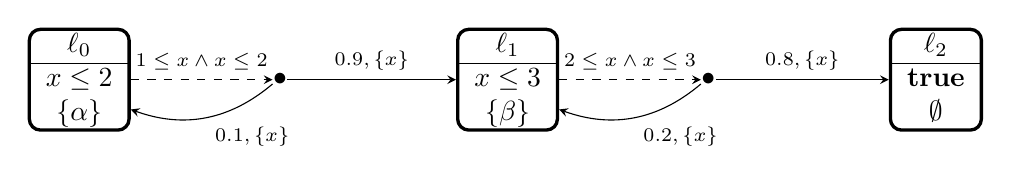
\begin{tikzpicture}[x = 1.7cm]
\node[location] (task1)         at (0,0)
{
\begin{tabular}{c}
$\loc_0$\\
\hline
$x\le 2$ \\
$\{\alpha\}$
\end{tabular}
};

\node[dec] (dec1)                    at (1.5,0)  {$\bullet$};

\node[location] (task2)         at (3.2,0)
{
\begin{tabular}{c}
$\loc_1$\\
\hline
$x\le 3$ \\
$\{\beta\}$
\end{tabular}
};

\node[dec] (dec2)                    at (4.7,0)  {$\bullet$};

\node[location] (finished)         at (6.4,0)
{
\begin{tabular}{c}
$\loc_2$\\
\hline
$\true$ \\
$\emptyset$
\end{tabular}
};

\draw[tran,dashed]    (task1)    to node[auto, font=\scriptsize] {$1\le x\wedge x\le 2$}    (dec1);
\draw[tran,bend left] (dec1)     to node[auto, font=\scriptsize] {$0.1,\{x\}$}     (task1);
\draw[tran]           (dec1)     to node[auto, font=\scriptsize] {$0.9, \{x\}$}    (task2);
\draw[tran,dashed]    (task2)    to node[auto, font=\scriptsize] {$2\le x\wedge x\le 3$}     (dec2);
\draw[tran,bend left] (dec2)     to node[auto, font=\scriptsize] {$0.2,\{x\}$}     (task2);
\draw[tran]           (dec2)     to node[auto, font=\scriptsize] {$0.8, \{x\}$}    (finished);
\end{tikzpicture}
}
\caption{A Task-Completion Example}
\label{fig:taskcompletion}
\vspace{-1em}
\end{figure}

A simple specification for {\sc Task-Completion} problem is that all tasks should be finished within a given amount of time with probability at least some given number.
We consider DTA-specifications which can express also the maximal completion time over individual tasks.
Example~\ref{ex:taskcompletiondta} explains this idea.

\begin{example}\label{ex:taskcompletiondta}
Consider the DTA depicted in Figure~\ref{fig:dtataskcompletion} which works as a specification for the PTA in Example~\ref{ex:taskcompletion}.
$q_i$'s ($1\le i\le 4$) are modes with $q_3$ being the final mode, $y,z$ are clocks and arrows between modes are rules.
For example, there are two rules emitting from $q_1$, one is $(q_1, \{\beta\}, y\le 3, \{y\}, q_2)$ and the other is
$(q_1, \{\alpha\}, \true,\emptyset, q_1)$.
$q_0$ is the initial mode to read the label of the initial location of a PTA in the product construction, and
$q_3$ is the final mode.
Note that this DTA does not satisfy the totality condition. However, this can be remedied by adding rules leading to a deadlock mode without changing the acceptance behaviour of the DTA.
In the product construction with the PTA in Example~\ref{ex:taskcompletion}, $y$ records completion time of individual tasks and $z$ records completion time of both tasks.
The specification then says that the PTA should complete the first task in $3$ time units (by $y\le 3$), the second task in $4$ time units (by $y\le 4$), and all the tasks in $6$ time units (by $z\le 6$).\qed
\end{example}

\begin{figure}
\centering
\resizebox{.5\textwidth}{!}{
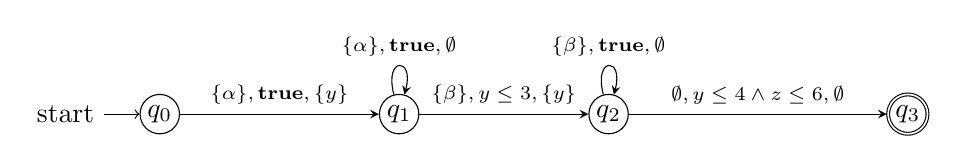
\begin{tikzpicture}[x = 3.8cm]
\node[mode,initial] (q0)         at (0.5,0)  {$\dtloc_0$};
\node[mode] (q1)         at (1.3,0)  {$\dtloc_1$};
\node[mode] (q2)         at (2,0)  {$\dtloc_2$};
\node[mode,accepting] (q3)         at (3,0)  {$\dtloc_3$};

\draw[tran] (q0)       to node[auto, font=\scriptsize] {$\{\alpha\}, \true, \{y\}$}      (q1);
\draw[tran, loop above] (q1)       to node[auto, font=\scriptsize] {$\{\alpha\}, \true, \emptyset$}  (q1);
\draw[tran] (q1)       to node[auto, font=\scriptsize] {$\{\beta\}, y\le 3,  \{y\}$} (q2);
\draw[tran, loop above] (q2)       to node[auto, font=\scriptsize] {$\{\beta\}, \true, \emptyset$}  (q2);
\draw[tran] (q2)       to node[auto, font=\scriptsize] {$\emptyset, y\le 4\wedge z\le 6,  \emptyset$} (q3);

\end{tikzpicture}
}
\caption{A DTA Specification for Example~\ref{ex:taskcompletion}}
\label{fig:dtataskcompletion}
\end{figure}
% \vspace{-0.8em}
\subsection{Robot Navigation}
% \vspace{-0.8em}
This case study is motivated from~\cite{DBLP:conf/tacas/BarbotCHKM11}.
In this case study, a robot is given the task to reach a destination in an unknown area.
Since the area is unknown,
the strategy the robot takes is to traverse the area randomly until the destination is reached.
Example~\ref{ex:robotnavigation} illustrates a simple setting on a $3$-by-$2$ grid.



\begin{example}\label{ex:robotnavigation}
Consider the robot-navigation problem depicted in Figure~\ref{fig:robotnavigation}.
On each tile, the time taken by a robot to leave the tile is always between $2$ and $3$ time-units.
The tile filled with black is an obstacle which cannot be entered.
The task for a robot is to start from the left-down corner of the $3$-by-$2$ grid, and move uniform-randomly to adjacent tiles excluding the obstacle until the upright corner is reached.
We assume that the robot does not always succeed to leave a tile, and the probability to successfully leave a tile is $0.9$.
The PTA modelling this problem is depicted in Figure~\ref{fig:ptarobotnavigation},
for which $x$ is the clock to measure the dwell-time on each tile, $\alpha,\beta$ are atomic propositions that distinguish adjacent tiles, and the way that the PTA is depicted is the same as for Example~\ref{ex:taskcompletion} and Figure~\ref{fig:taskcompletion}.
Each location $\loc_{i,j}$ corresponds to the situation that the robot stands in the tile $(i,j)$ (viewed as a coordinate in a two-dimensional plane) of the original grid.
The location $\loc_{2,1}$ is labelled $\emptyset$ to signify the destination.
Same as in Example~\ref{ex:taskcompletion}, we elaborate invariant conditions to disallow schedulers from repeatedly choosing time elapses. \qed
\end{example}

\begin{figure}
\begin{minipage}{0.3\textwidth}
\centering
~~\\
~\\
~\\
\scalebox{0.8}[0.8]{
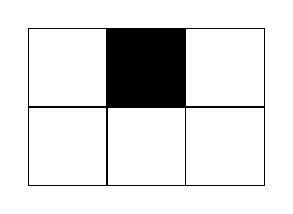
\begin{tikzpicture}[x = 1cm]
\begin{scope}
    \draw (0, 1) grid (3, 3);

    \setcounter{row}{1}
    \setrow{}{}{}
    \setrow{}{}{}
%    \node[anchor=center] at (1.5, -0.5) {Robot Navigation};
\end{scope}

\fill[black] (1,2) rectangle (2,3);

\end{tikzpicture}
}
\caption{A Robot Navigation}
\label{fig:robotnavigation}
\end{minipage}
\begin{minipage}{0.6\textwidth}
\centering
\scalebox{0.5}[0.5]{
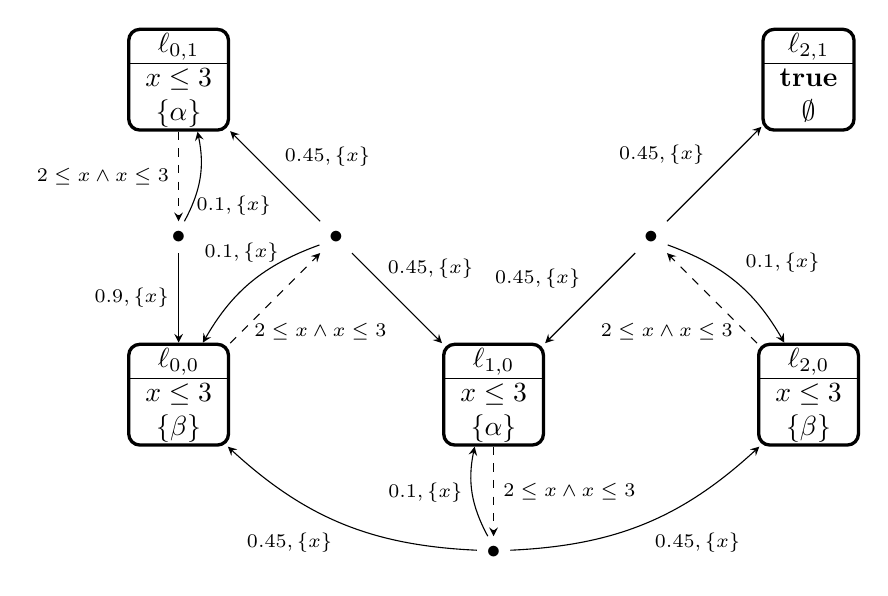
\begin{tikzpicture}[x=2cm, y=2cm]

\node[location] (q00)         at (0,0)
{
\begin{tabular}{c}
$\loc_{0,0}$\\
\hline
$x\le 3$ \\
$\{\beta\}$
\end{tabular}
};

\node           (dec00)       at (1, 1) {$\bullet$};

\node[location] (q01)         at (0,2)
{
\begin{tabular}{c}
$\loc_{0,1}$\\
\hline
$x\le 3$ \\
$\{\alpha\}$
\end{tabular}
};

\node           (dec01)       at (0, 1) {$\bullet$};

\node[location] (q10)         at (2,0)
{
\begin{tabular}{c}
$\loc_{1,0}$\\
\hline
$x\le 3$ \\
$\{\alpha\}$
\end{tabular}
};

\node (dec10) at (2,-1) {$\bullet$};

\node[location] (q20)         at (4,0)
{
\begin{tabular}{c}
$\loc_{2,0}$\\
\hline
$x\le 3$ \\
$\{\beta\}$
\end{tabular}
};

\node (dec20)  at (3,1) {$\bullet$};

\node[location] (q21)         at (4,2)
{
\begin{tabular}{c}
$\loc_{2,1}$\\
\hline
$\true$ \\
$\emptyset$
\end{tabular}
};

\node (sp1) at (0.9,0.4)  {{\scriptsize $2\le x\wedge x\le 3$}};
\node (sp2) at (3.1,0.4)  {{\scriptsize $2\le x\wedge x\le 3$}};
\node (dec00q00) at (0.4,0.9)  {{\scriptsize $0.1, \{x\}$}};
\node (dec01q01) at (0.35, 1.2)  {{\scriptsize $0.1, \{x\}$}};
\node (dec00q10) at (1.6, 0.8) {{\scriptsize $0.45, \{x\}$}};

%\node (dec21)  at (4,1) {$\bullet$};

\draw[tran]               (dec00)       to node[above right, font=\scriptsize]  {$0.45, \{x\}$}     (q01);
\draw[tran]               (dec00)       to      (q10);
\draw[tran,bend right=20] (dec00)       to      (q00);

\draw[tran]               (dec01)       to node[left, font=\scriptsize]  {$0.9, \{x\}$}               (q00);
\draw[tran,bend right=20] (dec01)       to                (q01);

\draw[tran,bend left=20]   (dec10)       to node[below left, font=\scriptsize]  {$0.45, \{x\}$}             (q00);
\draw[tran,bend right=20]  (dec10)       to node[below right, font=\scriptsize]  {$0.45, \{x\}$}             (q20);
\draw[tran,bend left=20]   (dec10)       to node[left, font=\scriptsize]  {$0.1, \{x\}$}           (q10);

\draw[tran]  (dec20)       to node[above left, font=\scriptsize]  {$0.45, \{x\}$}     (q10);
\draw[tran]  (dec20)       to node[auto, font=\scriptsize]  {$0.45, \{x\}$}     (q21);
\draw[tran, bend left=20]  (dec20)       to node[auto, font=\scriptsize]  {$0.1, \{x\}$}     (q20);

\draw[tran, dashed]  (q00)  to   (dec00);
\draw[tran, dashed]  (q01)  to node[left, font=\scriptsize]  {$2\le x\wedge x\le 3$}  (dec01);
\draw[tran, dashed]  (q10)  to node[auto, font=\scriptsize]  {$2\le x\wedge x\le 3$}  (dec10);
%\draw[tran, dashed]  (q21)  to node[auto, font=\scriptsize]  {$1\le x\wedge x\le 2$}  (dec21);
\draw[tran, dashed]  (q20)  to   (dec20);

\end{tikzpicture}
}
\caption{The PTA for Example~\ref{ex:robotnavigation}}
\label{fig:ptarobotnavigation}
\end{minipage}
\end{figure}



\begin{figure}
\centering
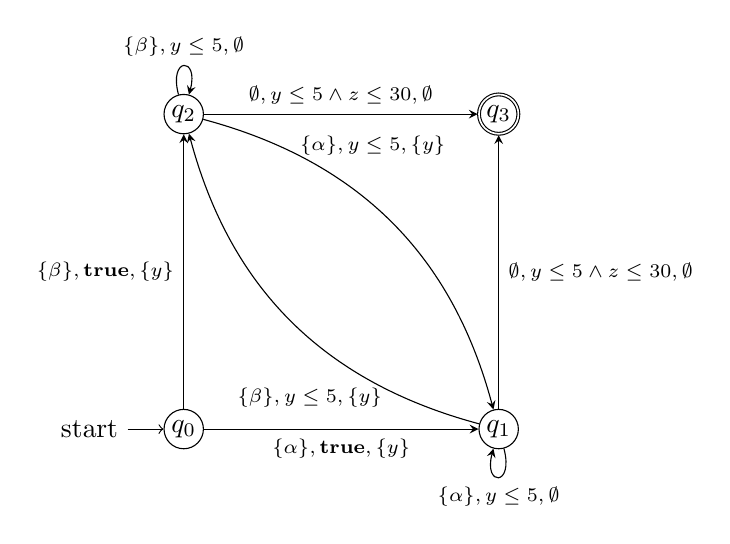
\begin{tikzpicture}[x = 4cm, y=4cm]

\node[mode,initial] (q0)         at (0,0)  {$\dtloc_0$};
\node[mode] (q1)         at (1,0)  {$\dtloc_1$};
\node[mode] (q2)         at (0,1)  {$\dtloc_2$};
\node[mode,accepting] (q3)         at (1,1)  {$\dtloc_3$};

\node (sp1) at (0.4, 0.1)  {{\scriptsize $\{\beta\}, y\le 5, \{y\}$}};
\node (sp2) at (0.6, 0.9) {{\scriptsize $\{\alpha\}, y\le 5, \{y\}$}};

\draw[tran] (q0)       to node[below, font=\scriptsize] {$\{\alpha\}, \true, \{y\}$}      (q1);
\draw[tran] (q0)       to node[left, font=\scriptsize] {$\{\beta\}, \true, \{y\}$}      (q2);
\draw[tran, loop below] (q1)      to node[auto, font=\scriptsize] {$\{\alpha\}, y\le 5, \emptyset$}  (q1);
\draw[tran, bend left]  (q1)      to    (q2);
\draw[tran, loop above] (q2)      to node[auto, font=\scriptsize] {$\{\beta\}, y\le 5, \emptyset$}   (q2);
\draw[tran, bend left]  (q2)       to    (q1);
\draw[tran] (q1)       to node[right, font=\scriptsize] {$\emptyset, y\le 5\wedge z\le 30,  \emptyset$} (q3);
\draw[tran] (q2)       to node[above, font=\scriptsize] {$\emptyset, y\le 5\wedge z\le 30,  \emptyset$} (q3);

\end{tikzpicture}
\caption{A DTA Specification for Example~\ref{ex:robotnavigation}}
\label{fig:dtarobotnavigation}
\end{figure}

Similar to the previous case study, we consider the specification that stress timing constraints on both dwell-time in individual tiles and total time to reach the destination for the robot.
\vspace{-0.5em}
\begin{example}
The DTA depicted in Figure~\ref{fig:dtarobotnavigation} specifies a property for the robot navigation described in Example~\ref{ex:robotnavigation}.
The way to render this DTA is the same as for Example~\ref{ex:taskcompletiondta}.
$q_0$ is the initial mode which reads the label of the initial tile where the robot lies and $q_3$ is the final mode.
The clock $y$ measures dwell-time on an individual tile, and the clock $z$ measures the total time to destination.
The property says that the robot should (i) never dwell on an individual tile more than $5$ time units (cf. the clock constraint $y\le 5$ and atomic propositions $\alpha,\beta$ that distinguishes adjacent tiles), and (ii) reach the upright corner within 30 time units (cf. the clock constraint $z\le 30$).\qed
\end{example}
\vspace{-0.8em}
In this section we conduct comprehensive experiments to emphasise the effectiveness of DIAL, including evaluations under white-box and black-box settings, robustness to unforeseen adversaries, robustness to unforeseen corruptions, transfer learning, and ablation studies. Finally, we present a new measurement to test the balance between robustness and natural accuracy, which we named $F_1$-robust score. 


\subsection{A case study on SVHN and CIFAR-100}
In the first part of our analysis, we conduct a case study experiment on two benchmark datasets: SVHN \citep{netzer2011reading} and CIFAR-100 \cite{krizhevsky2009learning}. We follow common experiment settings as in \cite{rice2020overfitting, wu2020adversarial}. We used the PreAct ResNet-18 \citep{he2016identity} architecture on which we integrate a domain classification layer. The adversarial training is done using 10-step PGD adversary with perturbation size of 0.031 and a step size of 0.003 for SVHN and 0.007 for CIFAR-100. The batch size is 128, weight decay is $7e^{-4}$ and the model is trained for 100 epochs. For SVHN, the initial learinnig rate is set to 0.01 and decays by a factor of 10 after 55, 75 and 90 iteration. For CIFAR-100, the initial learning rate is set to 0.1 and decays by a factor of 10 after 75 and 90 iterations. 
%We compared DIAL to \cite{madry2017towards} and TRADES \citep{zhang2019theoretically}. 
%The evaluation is done using Auto-Attack~\citep{croce2020reliable}, which is an ensemble of three white-box and one black-box parameter-free attacks, and various $\ell_{\infty}$ adversaries: PGD$^{20}$, PGD$^{100}$, PGD$^{1000}$ and CW$_{\infty}$ with step size of 0.003. 
Results are averaged over 3 restarts while omitting one standard deviation (which is smaller than 0.2\% in all experiments). As can be seen by the results in Tables~\ref{black-and_white-svhn} and \ref{black-and_white-cifar100}, DIAL presents consistent improvement in robustness (e.g., 5.75\% improved robustness on SVHN against AA) compared to the standard AT 
%under variety of attacks 
while also improving the natural accuracy. More results are presented in Appendix \ref{cifar100-svhn-appendix}.


\begin{table}[!ht]
  \caption{Robustness against white-box, black-box attacks and Auto-Attack (AA) on SVHN. Black-box attacks are generated using naturally trained surrogate model. Natural represents the naturally trained (non-adversarial) model.
  %and applied to the best performing robust models.
  }
  \vskip 0.1in
  \label{black-and_white-svhn}
  \centering
  \small
  \begin{tabular}{l@{\hspace{1\tabcolsep}}c@{\hspace{1\tabcolsep}}c@{\hspace{1\tabcolsep}}c@{\hspace{1\tabcolsep}}c@{\hspace{1\tabcolsep}}c@{\hspace{1\tabcolsep}}c@{\hspace{1\tabcolsep}}c@{\hspace{1\tabcolsep}}c@{\hspace{1\tabcolsep}}c@{\hspace{1\tabcolsep}}c}
    \toprule
    & & \multicolumn{4}{c}{White-box} & \multicolumn{4}{c}{Black-Box}  \\
    \cmidrule(r){3-6} 
    \cmidrule(r){7-10}
    Defense Model & Natural & PGD$^{20}$ & PGD$^{100}$  & PGD$^{1000}$  & CW$^{\infty}$ & PGD$^{20}$ & PGD$^{100}$ & PGD$^{1000}$  & CW$^{\infty}$ & AA \\
    \midrule
    NATURAL & 96.85 & 0 & 0 & 0 & 0 & 0 & 0 & 0 & 0 & 0 \\
    \midrule
    AT & 89.90 & 53.23 & 49.45 & 49.23 & 48.25 & 86.44 & 86.28 & 86.18 & 86.42 & 45.25 \\
    % TRADES & 90.35 & 57.10 & 54.13 & 54.08 & 52.19 & 86.89 & 86.73 & 86.57 & 86.70 &  49.50 \\
    $\DIAL_{\kl}$ (Ours) & 90.66 & \textbf{58.91} & \textbf{55.30} & \textbf{55.11} & \textbf{53.67} & 87.62 & 87.52 & 87.41 & 87.63 & \textbf{51.00} \\
    $\DIAL_{\ce}$ (Ours) & \textbf{92.88} & 55.26  & 50.82 & 50.54 & 49.66 & \textbf{89.12} & \textbf{89.01} & \textbf{88.74} & \textbf{89.10} &  46.52  \\
    \bottomrule
  \end{tabular}
\end{table}


\begin{table}[!ht]
  \caption{Robustness against white-box, black-box attacks and Auto-Attack (AA) on CIFAR100. Black-box attacks are generated using naturally trained surrogate model. Natural represents the naturally trained (non-adversarial) model.
  %and applied to the best performing robust models.
  }
  \vskip 0.1in
  \label{black-and_white-cifar100}
  \centering
  \small
  \begin{tabular}{l@{\hspace{1\tabcolsep}}c@{\hspace{1\tabcolsep}}c@{\hspace{1\tabcolsep}}c@{\hspace{1\tabcolsep}}c@{\hspace{1\tabcolsep}}c@{\hspace{1\tabcolsep}}c@{\hspace{1\tabcolsep}}c@{\hspace{1\tabcolsep}}c@{\hspace{1\tabcolsep}}c@{\hspace{1\tabcolsep}}c}
    \toprule
    & & \multicolumn{4}{c}{White-box} & \multicolumn{4}{c}{Black-Box}  \\
    \cmidrule(r){3-6} 
    \cmidrule(r){7-10}
    Defense Model & Natural & PGD$^{20}$ & PGD$^{100}$  & PGD$^{1000}$  & CW$^{\infty}$ & PGD$^{20}$ & PGD$^{100}$ & PGD$^{1000}$  & CW$^{\infty}$ & AA \\
    \midrule
    NATURAL & 79.30 & 0 & 0 & 0 & 0 & 0 & 0 & 0 & 0 & 0 \\
    \midrule
    AT & 56.73 & 29.57 & 28.45 & 28.39 & 26.6 & 55.52 & 55.29 & 55.26 & 55.40 & 24.12 \\
    % TRADES & 58.24 & 30.10 & 29.66 & 29.64 & 25.97 & 57.05 & 56.71 & 56.67 & 56.77 & 24.92 \\
    $\DIAL_{\kl}$ (Ours) & 58.47 & \textbf{31.19} & \textbf{30.50} & \textbf{30.42} & \textbf{26.91} & 57.16 & 56.81 & 56.80 & 57.00 & \textbf{25.87} \\
    $\DIAL_{\ce}$ (Ours) & \textbf{60.77} & 27.87 & 26.66 & 26.61 & 25.98 & \textbf{59.48} & \textbf{59.06} & \textbf{58.96} & \textbf{59.20} & 23.51  \\
    \bottomrule
  \end{tabular}
\end{table}


% \begin{table}[!ht]
%   \caption{Robustness comparison of DIAL to Madry et al. and TRADES defense models on the SVHN dataset under different PGD white-box attacks and the ensemble Auto-Attack (AA).}
%   \label{svhn}
%   \centering
%   \begin{tabular}{llllll|l}
%     \toprule
%     \cmidrule(r){1-5}
%     Defense Model & Natural & PGD$^{20}$ & PGD$^{100}$ & PGD$^{1000}$ & CW$_{\infty}$ & AA\\
%     \midrule
%     $\DIAL_{\kl}$ (Ours) & $\mathbf{90.66}$ & $\mathbf{58.91}$ & $\mathbf{55.30}$ & $\mathbf{55.12}$ & $\mathbf{53.67}$  & $\mathbf{51.00}$  \\
%     Madry et al. & 89.90 & 53.23 & 49.45 & 49.23 & 48.25 & 45.25  \\
%     TRADES & 90.35 & 57.10 & 54.13 & 54.08 & 52.19 & 49.50 \\
%     \bottomrule
%   \end{tabular}
% \end{table}


\subsection{Performance comparison on CIFAR-10} \label{defence-settings}
In this part, we evaluate the performance of DIAL compared to other well-known methods on CIFAR-10. 
%To be consistent with other methods, 
We follow the same experiment setups as in~\cite{madry2017towards, wang2019improving, zhang2019theoretically}. When experiment settings are not identical between tested methods, we choose the most commonly used settings, and apply it to all experiments. This way, we keep the comparison as fair as possible and avoid reporting changes in results which are caused by inconsistent experiment settings \citep{pang2020bag}. To show that our results are not caused because of what is referred to as \textit{obfuscated gradients}~\citep{athalye2018obfuscated}, we evaluate our method with same setup as in our defense model, under strong attacks (e.g., PGD$^{1000}$) in both white-box, black-box settings, Auto-Attack ~\citep{croce2020reliable}, unforeseen "natural" corruptions~\citep{hendrycks2018benchmarking}, and unforeseen adversaries. To make sure that the reported improvements are not caused by \textit{adversarial overfitting}~\citep{rice2020overfitting}, we report best robust results for each method on average of 3 restarts, while omitting one standard deviation (which is smaller than 0.2\% in all experiments). Additional results for CIFAR-10 as well as comprehensive evaluation on MNIST can be found in Appendix \ref{mnist-results} and \ref{additional_res}.
%To further keep the comparison consistent, we followed the same attack settings for all methods.


\begin{table}[ht]
  \caption{Robustness against white-box, black-box attacks and Auto-Attack (AA) on CIFAR-10. Black-box attacks are generated using naturally trained surrogate model. Natural represents the naturally trained (non-adversarial) model.
  %and applied to the best performing robust models.
  }
  \vskip 0.1in
  \label{black-and_white-cifar}
  \centering
  \small
  \begin{tabular}{cccccccc@{\hspace{1\tabcolsep}}c}
    \toprule
    & & \multicolumn{3}{c}{White-box} & \multicolumn{3}{c}{Black-Box} \\
    \cmidrule(r){3-5} 
    \cmidrule(r){6-8}
    Defense Model & Natural & PGD$^{20}$ & PGD$^{100}$ & CW$^{\infty}$ & PGD$^{20}$ & PGD$^{100}$ & CW$^{\infty}$ & AA \\
    \midrule
    NATURAL & 95.43 & 0 & 0 & 0 & 0 & 0 & 0 &  0 \\
    \midrule
    TRADES & 84.92 & 56.60 & 55.56 & 54.20 & 84.08 & 83.89 & 83.91 &  53.08 \\
    MART & 83.62 & 58.12 & 56.48 & 53.09 & 82.82 & 82.52 & 82.80 & 51.10 \\
    AT & 85.10 & 56.28 & 54.46 & 53.99 & 84.22 & 84.14 & 83.92 & 51.52 \\
    ATDA & 76.91 & 43.27 & 41.13 & 41.01 & 75.59 & 75.37 & 75.35 & 40.08\\
    $\DIAL_{\kl}$ (Ours) & 85.25 & $\mathbf{58.43}$ & $\mathbf{56.80}$ & $\mathbf{55.00}$ & 84.30 & 84.18 & 84.05 & \textbf{53.75} \\
    $\DIAL_{\ce}$ (Ours)  & $\mathbf{89.59}$ & 54.31 & 51.67 & 52.04 &$ \mathbf{88.60}$ & $\mathbf{88.39}$ & $\mathbf{88.44}$ & 49.85 \\
    \midrule
    $\DIAL_{\awp}$ (Ours) & $\mathbf{85.91}$ & $\mathbf{61.10}$ & $\mathbf{59.86}$ & $\mathbf{57.67}$ & $\mathbf{85.13}$ & $\mathbf{84.93}$ & $\mathbf{85.03}$  & \textbf{56.78} \\
    $\TRADES_{\awp}$ & 85.36 & 59.27 & 59.12 & 57.07 & 84.58 & 84.58 & 84.59 & 56.17 \\
    \bottomrule
  \end{tabular}
\end{table}



\paragraph{CIFAR-10 setup.} We use the wide residual network (WRN-34-10)~\citep{zagoruyko2016wide} architecture. %used in the experiments of~\cite{madry2017towards, wang2019improving, zhang2019theoretically}. 
Sidelong this architecture, we integrate a domain classification layer. To generate the adversarial domain dataset, we use a perturbation size of $\epsilon=0.031$. We apply 10 of inner maximization iterations with perturbation step size of 0.007. Batch size is set to 128, weight decay is set to $7e^{-4}$, and the model is trained for 100 epochs. Similar to the other methods, the initial learning rate was set to 0.1, and decays by a factor of 10 at iterations 75 and 90. 
%For being consistent with other methods, the natural images are padded with 4-pixel padding with 32-random crop and random horizontal flip. Furthermore, all methods are trained using SGD with momentum 0.9. For $\DIAL_{\kl}$, we balance the robust loss with $\lambda=6$ and the domains loss with $r=4$. For $\DIAL_{\ce}$, we balance the robust loss with $\lambda=1$ and the domains loss with $r=2$. 
%We also introduce a version of our method that incorporates the AWP double-perturbation mechanism, named DIAL-AWP.
%which is trained using the same learning rate schedule used in ~\cite{wu2020adversarial}, where the initial 0.1 learning rate decays by a factor of 10 after 100 and 150 iterations. 
See Appendix \ref{cifar10-additional-setup} for additional details.

\begin{table}[ht]
  \caption{Black-box attack using the adversarially trained surrogate models on CIFAR-10.}
  \vskip 0.1in
  \label{black-box-cifar-adv}
  \centering
  \small
  \begin{tabular}{ll|c}
    \toprule
    \cmidrule(r){1-2}
    Surrogate (source) model & Target model & robustness \% \\
    % \midrule
    \midrule
    TRADES & $\DIAL_{\ce}$ & $\mathbf{67.77}$ \\
    $\DIAL_{\ce}$ & TRADES & 65.75 \\
    \midrule
    MART & $\DIAL_{\ce}$ & $\mathbf{70.30}$ \\
    $\DIAL_{\ce}$ & MART & 64.91 \\
    \midrule
    AT & $\DIAL_{\ce}$ & $\mathbf{65.32}$ \\
    $\DIAL_{\ce}$ & AT  & 63.54 \\
    \midrule
    ATDA & $\DIAL_{\ce}$ & $\mathbf{66.77}$ \\
    $\DIAL_{\ce}$ & ATDA & 52.56 \\
    \bottomrule
  \end{tabular}
\end{table}

\paragraph{White-box/Black-box robustness.} 
%We evaluate all defense models using Auto-Attack, PGD$^{20}$, PGD$^{100}$, PGD$^{1000}$ and CW$_{\infty}$ with step size 0.003. We constrain all attacks by the same perturbation $\epsilon=0.031$. 
As reported in Table~\ref{black-and_white-cifar} and Appendix~\ref{additional_res}, our method achieves better robustness compared to the other methods. Specifically, in the white-box settings, our method improves robustness over~\citet{madry2017towards} and TRADES by 2\% 
%using the common PGD$^{20}$ attack 
while keeping higher natural accuracy. We also observe better natural accuracy of 1.65\% over MART while also achieving better robustness over all attacks. Moreover, our method presents significant improvement of up to 15\% compared to the the domain invariant method suggested by~\citet{song2018improving} (ATDA).
%in both natural and robust accuracy. 
When incorporating 
%the double-perturbation mechanism of 
AWP, our method improves the results of $\TRADES_{\awp}$ by almost 2\%.
%and reaches state-of-the-art results for robust models with no additional data. 
% Additional results are available in Appendix~\ref{additional_res}.
When tested on black-box settings, $\DIAL_{\ce}$ presents a significant improvement of more than 4.4\% over the second-best performing method, and up to 13\%. In Table~\ref{black-box-cifar-adv}, we also present the black-box results when the source model is taken from one of the adversarially trained models. %Then, we compare our model to each one of them both as the source model and target model. 
In addition to the improvement in black-box robustness, $\DIAL_{\ce}$ also manages to achieve better clean accuracy of more than 4.5\% over the second-best performing method.
% Moreover, based on the auto-attack leader-board \footnote{\url{https://github.com/fra31/auto-attack}}, our method achieves the 1st place among models without additional data using the WRN-34-10 architecture.

% \begin{table}
%   \caption{White-box robustness on CIFAR-10 using WRN-34-10}
%   \label{white-box-cifar-10}
%   \centering
%   \begin{tabular}{lllll}
%     \toprule
%     \cmidrule(r){1-2}
%     Defense Model & Natural & PGD$^{20}$ & PGD$^{100}$ & PGD$^{1000}$ \\
%     \midrule
%     TRADES ~\cite{zhang2019theoretically} & 84.92  & 56.6 & 55.56 & 56.43  \\
%     MART ~\cite{wang2019improving} & 83.62  & 58.12 & 56.48 & 56.55  \\
%     Madry et al. ~\cite{madry2017towards} & 85.1  & 56.28 & 54.46 & 54.4  \\
%     Song et al. ~\cite{song2018improving} & 76.91 & 43.27 & 41.13 & 41.02  \\
%     $\DIAL_{\ce}$ (Ours) & $ \mathbf{90}$  & 52.12 & 48.88 & 48.78  \\
%     $\DIAL_{\kl}$ (Ours) & 85.25 & $\mathbf{58.43}$ & $\mathbf{56.8}$ & $\mathbf{56.73}$ \\
%     \midrule
%     $\DIAL_{\kl}$+AWP (Ours) & $\mathbf{85.91}$ & $\mathbf{61.1}$ & - & -  \\
%     TRADES+AWP \cite{wu2020adversarial} & 85.36 & 59.27 & 59.12 & -  \\
%     % MART + AWP & 84.43 & 60.68 & 59.32 & -  \\
%     \bottomrule
%   \end{tabular}
% \end{table}


% \begin{table}
%   \caption{White-box robustness on MNIST}
%   \label{white-box-mnist}
%   \centering
%   \begin{tabular}{llllll}
%     \toprule
%     \cmidrule(r){1-2}
%     Defense Model & Natural & PGD$^{40}$ & PGD$^{100}$ & PGD$^{1000}$ \\
%     \midrule
%     TRADES ~\cite{zhang2019theoretically} & 99.48 & 96.07 & 95.52 & 95.22 \\
%     MART ~\cite{wang2019improving} & 99.38  & 96.99 & 96.11 & 95.74  \\
%     Madry et al. ~\cite{madry2017towards} & 99.41  & 96.01 & 95.49 & 95.36 \\
%     Song et al. ~\cite{song2018improving}  & 98.72 & 96.82 & 96.26 & 96.2  \\
%     $\DIAL_{\kl}$ (Ours) & 99.46 & 97.05 & 96.06 & 95.99  \\
%     $\DIAL_{\ce}$ (Ours) & $\mathbf{99.49}$  & $\mathbf{97.38}$ & $\mathbf{96.45}$ & $\mathbf{96.33}$ \\
%     \bottomrule
%   \end{tabular}
% \end{table}


% \paragraph{Attacking MNIST.} For consistency, we use the same perturbation and step sizes. For MNIST, we use $\epsilon=0.3$ and step size of $0.01$. The natural accuracy of our surrogate (source) model is 99.51\%. Attacks results are reported in Table~\ref{black-and_white-mnist}. It is worth noting that the improvement margin is not conclusive on MNIST as it is on CIFAR-10, which is a more complex task.

% \begin{table}
%   \caption{Black-box robustness on MNIST and CIFAR-10 using naturally trained surrogate model and best performing robust models}
%   \label{black-box-mnist-cifar}
%   \centering
%   \begin{tabular}{lllllll}
%     \toprule
%     & \multicolumn{3}{c}{MNIST} & \multicolumn{3}{c}{CIFAR-10} \\
%     \cmidrule(r){2-4} 
%     \cmidrule(r){5-7}  
%     Defense Model & PGD$^{40}$ & PGD$^{100}$ & PGD$^{1000}$ & PGD$^{20}$ & PGD$^{100}$ & PGD$^{1000}$ \\
%     \midrule
%     TRADES ~\cite{zhang2019theoretically} & 98.12 & 97.86 & 97.81 & 84.08 & 83.89 & 83.8 \\
%     MART ~\cite{wang2019improving} & 98.16 & 97.96 & 97.89  & 82.82 & 82.52 & 82.47 \\
%     Madry et al. ~\cite{madry2017towards}  & 98.05 & 97.73 & 97.78 & 84.22 & 84.14 & 83.96 \\
%     Song et al. ~\cite{song2018improving} & 97.74 & 97.28 & 97.34 & 75.59 & 75.37 & 75.11 \\
%     $\DIAL_{\kl}$ (Ours) & 98.14 & 97.83 & 97.87  & 84.3 & 84.18 & 84.0 \\
%     $\DIAL_{\ce}$ (Ours)  & $\mathbf{98.37}$ & $\mathbf{98.12}$ & $\mathbf{98.05}$  & $\mathbf{89.13}$ & $\mathbf{88.89}$ & $\mathbf{88.78}$ \\
%     \bottomrule
%   \end{tabular}
% \end{table}



% \subsubsection{Ensemble attack} In addition to the white-box and black-box settings, we evaluate our method on the Auto-Attack ~\citep{croce2020reliable} using $\ell_{\infty}$ threat model with perturbation $\epsilon=0.031$. Auto-Attack is an ensemble of parameter-free attacks. It consists of three white-box attacks: APGD-CE which is a step size-free version of PGD on the cross-entropy ~\citep{croce2020reliable}. APGD-DLR which is a step size-free version of PGD on the DLR loss ~\citep{croce2020reliable} and FAB which  minimizes the norm of the adversarial perturbations, and one black-box attack: square attack which is a query-efficient black-box attack ~\citep{andriushchenko2020square}. Results are presented in Table~\ref{auto-attack}. Based on the auto-attack leader-board \footnote{\url{https://github.com/fra31/auto-attack}}, our method achieves the 1st place among models without additional data using the WRN-34-10 architecture.

%Additional results can be found in Appendix ~\ref{additional_res}.

% \begin{table}
%   \caption{Auto-Attack (AA) on CIFAR-10 with perturbation size $\epsilon=0.031$ with $\ell_{\infty}$ threat model}
%   \label{auto-attack}
%   \centering
%   \begin{tabular}{lll}
%     \toprule
%     \cmidrule(r){1-2}
%     Defense Model & AA \\
%     \midrule
%     TRADES ~\cite{zhang2019theoretically} & 53.08  \\
%     MART ~\cite{wang2019improving} & 51.1  \\
%     Madry et al. ~\cite{madry2017towards} & 51.52    \\
%     Song et al.   ~\cite{song2018improving} & 40.18 \\
%     $\DIAL_{\ce}$ (Ours) & 47.33  \\
%     $\DIAL_{\kl}$ (Ours) & $\mathbf{53.75}$ \\
%     \midrule
%     DIAL-AWP (Ours) & $\mathbf{56.78}$ \\
%     TRADES-AWP \cite{wu2020adversarial} & 56.17 \\
%     \bottomrule
%   \end{tabular}
% \end{table}


% \begin{table}[!ht]
%   \caption{Auto-Attack (AA) Robustness (\%) on CIFAR-10 with $\epsilon=0.031$ using an $\ell_{\infty}$ threat model}
%   \label{auto-attack}
%   \centering
%   \begin{tabular}{cccccc|cc}
%     \toprule
%     % \multicolumn{8}{c}{Defence Model}  \\
%     % \cmidrule(r){1-8} 
%     TRADES & MART & Madry & Song & $\DIAL_{\ce}$ & $\DIAL_{\kl}$ & DIAL-AWP  & TRADES-AWP\\
%     \midrule
%     53.08 & 51.10 & 51.52 &  40.08 & 47.33  & $\mathbf{53.75}$ & $\mathbf{56.78}$ & 56.17 \\

%     \bottomrule
%   \end{tabular}
% \end{table}

% \begin{table}[!ht]
% \caption{$F_1$-robust measurement using PGD$^{20}$ attack in white-box and black-box settings on CIFAR-10}
%   \label{f1-robust}
%   \centering
%   \begin{tabular}{ccccccc|cc}
%     \toprule
%     % \multicolumn{8}{c}{Defence Model}  \\
%     % \cmidrule(r){1-8} 
%     Defense Model & TRADES & MART & Madry & Song & $\DIAL_{\kl}$ & $\DIAL_{\ce}$ & DIAL-AWP  & TRADES-AWP\\
%     \midrule
%     White-box & 0.659 & 0.666 & 0.657 & 0.518 & $\mathbf{0.675}$  & 0.643 & $\mathbf{0.698}$ & 0.682 \\
%     Black-box & 0.844 & 0.831 & 0.846 & 0.761 & 0.847 & $\mathbf{0.895}$ & $\mathbf{0.854}$ &  0.849 \\
%     \bottomrule
%   \end{tabular}
% \end{table}

\subsubsection{Robustness to Unforeseen Attacks and Corruptions}
\paragraph{Unforeseen Adversaries.} To further demonstrate the effectiveness of our approach, we test our method against various adversaries that were not used during the training process. We attack the model under the white-box settings with $\ell_{2}$-PGD, $\ell_{1}$-PGD, $\ell_{\infty}$-DeepFool and $\ell_{2}$-DeepFool \citep{moosavi2016deepfool} adversaries using Foolbox \citep{rauber2017foolbox}. We applied commonly used attack budget 
%(perturbation for PGD adversaries and overshot for DeepFool adversaries) 
with 20 and 50 iterations for PGD and DeepFool, respectively.
Results are presented in Table \ref{unseen-attacks}. As can be seen, our approach  gains an improvement of up to 4.73\% over the second best method under the various attack types and an average improvement of 3.7\% over all threat models.


\begin{table}[ht]
  \caption{Robustness on CIFAR-10 against unseen adversaries under white-box settings.}
  \vskip 0.1in
  \label{unseen-attacks}
  \centering
%   \small
  \begin{tabular}{c@{\hspace{1.5\tabcolsep}}c@{\hspace{1.5\tabcolsep}}c@{\hspace{1.5\tabcolsep}}c@{\hspace{1.5\tabcolsep}}c@{\hspace{1.5\tabcolsep}}c@{\hspace{1.5\tabcolsep}}c@{\hspace{1.5\tabcolsep}}c}
    \toprule
    Threat Model & Attack Constraints & $\DIAL_{\kl}$ & $\DIAL_{\ce}$ & AT & TRADES & MART & ATDA \\
    \midrule
    \multirow{2}{*}{$\ell_{2}$-PGD} & $\epsilon=0.5$ & 76.05 & \textbf{80.51} & 76.82 & 76.57 & 75.07 & 66.25 \\
    & $\epsilon=0.25$ & 80.98 & \textbf{85.38} & 81.41 & 81.10 & 80.04 & 71.87 \\\midrule
    \multirow{2}{*}{$\ell_{1}$-PGD} & $\epsilon=12$ & 74.84 & \textbf{80.00} & 76.17 & 75.52 & 75.95 & 65.76 \\
    & $\epsilon=7.84$ & 78.69 & \textbf{83.62} & 79.86 & 79.16 & 78.55 & 69.97 \\
    \midrule
    $\ell_{2}$-DeepFool & overshoot=0.02 & 84.53 & \textbf{88.88} & 84.15 & 84.23 & 82.96 & 76.08 \\\midrule
    $\ell_{\infty}$-DeepFool & overshoot=0.02 & 68.43 & \textbf{69.50} & 67.29 & 67.60 & 66.40 & 57.35 \\
    \bottomrule
  \end{tabular}
\end{table}


%%%%%%%%%%%%%%%%%%%%%%%%% conference version %%%%%%%%%%%%%%%%%%%%%%%%%%%%%%%%%%%%%
\paragraph{Unforeseen Corruptions.}
We further demonstrate that our method consistently holds against unforeseen ``natural'' corruptions, consists of 18 unforeseen diverse corruption types proposed by \citet{hendrycks2018benchmarking} on CIFAR-10, which we refer to as CIFAR10-C. The CIFAR10-C benchmark covers noise, blur, weather, and digital categories. As can be shown in Figure \ref{corruption}, our method gains a significant and consistent improvement over all the other methods. Our method leads to an average improvement of 4.7\% with minimum improvement of 3.5\% and maximum improvement of 5.9\% compared to the second best method over all unforeseen attacks. See Appendix \ref{corruptions-apendix} for the full experiment results.


\begin{figure}[h]
 \centering
  \includegraphics[width=0.4\textwidth]{figures/spider_full.png}
%   \caption{Summary of accuracy over all unforeseen corruptions compared to the second and third best performing methods.}
  \caption{Accuracy comparison over all unforeseen corruptions.}
  \label{corruption}
\end{figure}


%%%%%%%%%%%%%%%%%%%%%%%%% conference version %%%%%%%%%%%%%%%%%%%%%%%%%%%%%%%%%%%%%

%%%%%%%%%%%%%%%%%%%%%%%%% Arxiv version %%%%%%%%%%%%%%%%%%%%%%%%%%%%%%%%%%%%%
% \newpage
% \paragraph{Unforeseen Corruptions.}
% We further demonstrate that our method consistently holds against unforeseen "natural" corruptions, consists of 18 unforeseen diverse corruption types proposed by \cite{hendrycks2018benchmarking} on CIFAR-10, which we refer to as CIFAR10-C. The CIFAR10-C benchmark covers noise, blur, weather, and digital categories. As can be shown in Figure  \ref{spider-full-graph}, our method gains a significant and consistent improvement over all the other methods. Our approach leads to an average improvement of 4.7\% with minimum improvement of 3.5\% and maximum improvement of 5.9\% compared to the second best method over all unforeseen attacks. Full accuracy results against unforeseen corruptions are presented in Tables \ref{corruption-table1} and \ref{corruption-table2}. 

% \begin{table}[!ht]
%   \caption{Accuracy (\%) against unforeseen corruptions.}
%   \label{corruption-table1}
%   \centering
%   \tiny
%   \begin{tabular}{lcccccccccccccccccc}
%     \toprule
%     Defense Model & brightness & defocus blur & fog & glass blur & jpeg compression & motion blur & saturate & snow & speckle noise  \\
%     \midrule
%     TRADES & 82.63 & 80.04 & 60.19 & 78.00 & 82.81 & 76.49 & 81.53 & 80.68 & 80.14 \\
%     MART & 80.76 & 78.62 & 56.78 & 76.60 & 81.26 & 74.58 & 80.74 & 78.22 & 79.42 \\
%     AT &  83.30 & 80.42 & 60.22 & 77.90 & 82.73 & 76.64 & 82.31 & 80.37 & 80.74 \\
%     ATDA & 72.67 & 69.36 & 45.52 & 64.88 & 73.22 & 63.47 & 72.07 & 68.76 & 72.27 \\
%     DIAL (Ours)  & \textbf{87.14} & \textbf{84.84} & \textbf{66.08} & \textbf{81.82} & \textbf{87.07} & \textbf{81.20} & \textbf{86.45} & \textbf{84.18} & \textbf{84.94} \\
%     \bottomrule
%   \end{tabular}
% \end{table}


% \begin{table}[!ht]
%   \caption{Accuracy (\%) against unforeseen corruptions.}
%   \label{corruption-table2}
%   \centering
%   \tiny
%   \begin{tabular}{lcccccccccccccccccc}
%     \toprule
%     Defense Model & contrast & elastic transform & frost & gaussian noise & impulse noise & pixelate & shot noise & spatter & zoom blur \\
%     \midrule
%     TRADES & 43.11 & 79.11 & 76.45 & 79.21 & 73.72 & 82.73 & 80.42 & 80.72 & 78.97 \\
%     MART & 41.22 & 77.77 & 73.07 & 78.30 & 74.97 & 81.31 & 79.53 & 79.28 & 77.8 \\
%     AT & 43.30 & 79.58 & 77.53 & 79.47 & 73.76 & 82.78 & 80.86 & 80.49 & 79.58 \\
%     ATDA & 36.06 & 67.06 & 62.56 & 70.33 & 64.63 & 73.46 & 72.28 & 70.50 & 67.31 \\
%     DIAL (Ours) & \textbf{48.84} & \textbf{84.13} & \textbf{81.76} & \textbf{83.76} & \textbf{78.26} & \textbf{87.24} & \textbf{85.13} & \textbf{84.84} & \textbf{83.93}  \\
%     \bottomrule
%   \end{tabular}
% \end{table}


% \begin{figure}[!ht]
%   \centering
%   \includegraphics[width=9cm]{figures/spider_full.png}
%   \caption{Accuracy comparison with all tested methods over unforeseen corruptions.}
%   \label{spider-full-graph}
% \end{figure}
% %%%%%%%%%%%%%%%%%%%%%%%%% Arxiv version %%%%%%%%%%%%%%%%%%%%%%%%%%%%%%%%%%%%%
%%%%%%%%%%%%%%%%%%%%%%%%% Arxiv version %%%%%%%%%%%%%%%%%%%%%%%%%%%%%%%%%%%%%

\subsubsection{Transfer Learning}
Recent works \citep{salman2020adversarially,utrera2020adversarially} suggested that robust models transfer better on standard downstream classification tasks. In Table \ref{transfer-res} we demonstrate the advantage of our method when applied for transfer learning across CIFAR10 and CIFAR100 using the common linear evaluation protocol. see Appendix \ref{transfer-learning-settings} for detailed settings.

\begin{table}[H]
  \caption{Transfer learning results comparison.}
  \vskip 0.1in
  \label{transfer-res}
  \centering
  \small
\begin{tabular}{c|c|c|c}
\toprule

\multicolumn{2}{l}{} & \multicolumn{2}{c}{Target} \\
\cmidrule(r){3-4}
Source & Defence Model & CIFAR10 & CIFAR100 \\
\midrule
\multirow{3}{*}{CIFAR10} & DIAL & \multirow{3}{*}{-} & \textbf{28.57} \\
 & AT &  & 26.95  \\
 & TRADES &  & 25.40  \\
 \midrule
\multirow{3}{*}{CIFAR100} & DIAL & \textbf{73.68} & \multirow{3}{*}{-} \\
 & AT & 71.41 & \\
 & TRADES & 71.42 &  \\
%  \midrule
% \multirow{3}{}{SVHN} & DIAL &  &  & \multirow{3}{}{-} \\
%  & Madry et al. &  &  &  \\
%  & TRADES &  &  &  \\ 
\bottomrule
\end{tabular}
\end{table}


\subsubsection{Modularity and Ablation Studies}

We note that the domain classifier is a modular component that can be integrated into existing models for further improvements. Removing the domain head and related loss components from the different DIAL formulations results in some common adversarial training techniques. For $\DIAL_{\kl}$, removing the domain and related loss components results in the formulation of TRADES. For $\DIAL_{\ce}$, removing the domain and related loss components results in the original formulation of the standard adversarial training, and for $\DIAL_{\awp}$ the removal results in $\TRADES_{\awp}$. Therefore, the ablation studies will demonstrate the effectiveness of combining DIAL on top of different adversarial training methods. 

We investigate the contribution of the additional domain head component introduced in our method. Experiment configuration are as in \ref{defence-settings}, and robust accuracy is based on white-box PGD$^{20}$ on CIFAR-10 dataset. We remove the domain head from both $\DIAL_{\kl}$, $\DIAL_{\awp}$, and $\DIAL_{\ce}$ (equivalent to $r=0$) and report the natural and robust accuracy. We perform 3 random restarts and omit one standard deviation from the results. Results are presented in Figure \ref{ablation}. All DIAL variants exhibits stable improvements on both natural accuracy and robust accuracy. $\DIAL_{\ce}$, $\DIAL_{\kl}$, and $\DIAL_{\awp}$ present an improvement of 1.82\%, 0.33\%, and 0.55\% on natural accuracy and an improvement of 2.5\%, 1.87\%, and 0.83\% on robust accuracy, respectively. This evaluation empirically demonstrates the benefits of incorporating DIAL on top of different adversarial training techniques.
% \paragraph{semi-supervised extensions.} Since the domain classifier does not require the class labels, we argue that additional unlabeled data can be leveraged in future work.
%for improved results. 

\begin{figure}[ht]
  \centering
  \includegraphics[width=0.35\textwidth]{figures/ablation_graphs3.png}
  \caption{Ablation studies for $\DIAL_{\kl}$, $\DIAL_{\ce}$, and $\DIAL_{\awp}$ on CIFAR-10. Circle represent the robust-natural accuracy without using DIAL, and square represent the robust-natural accuracy when incorporating DIAL.
  %to further investigate the impact of the domain head and loss on natural and robust accuracy.
  }
  \label{ablation}
\end{figure}

\subsubsection{Visualizing DIAL}
To further illustrate the superiority of our method, we visualize the model outputs from the different methods on both natural and adversarial test data.
% adversarial test data generated using PGD$^{20}$ white-box attack with step size 0.003 and $\epsilon=0.031$ on CIFAR-10. 
Figure~\ref{tsne1} shows the embedding received after applying t-SNE ~\citep{van2008visualizing} with two components on the model output for our method and for TRADES. DIAL seems to preserve strong separation between classes on both natural test data and adversarial test data. Additional illustrations for the other methods are attached in Appendix~\ref{additional_viz}. 

\begin{figure}[h]
\centering
  \subfigure[\textbf{DIAL} on natural logits]{\includegraphics[width=0.21\textwidth]{figures/domain_ce_test.png}}
  \hspace{0.03\textwidth}
  \subfigure[\textbf{DIAL} on adversarial logits]{\includegraphics[width=0.21\textwidth]{figures/domain_ce_adversarial.png}}
  \hspace{0.03\textwidth}
    \subfigure[\textbf{TRADES} on natural logits]{\includegraphics[width=0.21\textwidth]{figures/trades_test.png}}
    \hspace{0.03\textwidth}
    \subfigure[\textbf{TRADES} on adversarial logits]{\includegraphics[width=0.21\textwidth]{figures/trades_adversarial.png}}
  \caption{t-SNE embedding of model output (logits) into two-dimensional space for DIAL and TRADES using the CIFAR-10 natural test data and the corresponding PGD$^{20}$ generated adversarial examples.}
  \label{tsne1}
\end{figure}


% \begin{figure}[ht]
% \centering
%   \begin{subfigure}{4cm}
%     \centering\includegraphics[width=3.3cm]{figures/domain_ce_test.png}
%     \caption{\textbf{DIAL} on nat. examples}
%   \end{subfigure}
%   \begin{subfigure}{4cm}
%     \centering\includegraphics[width=3.3cm]{figures/domain_ce_adversarial.png}
%     \caption{\textbf{DIAL} on adv. examples}
%   \end{subfigure}
  
%   \begin{subfigure}{4cm}
%     \centering\includegraphics[width=3.3cm]{figures/trades_test.png}
%     \caption{\textbf{TRADES} on nat. examples}
%   \end{subfigure}
%   \begin{subfigure}{4cm}
%     \centering\includegraphics[width=3.3cm]{figures/trades_adversarial.png}
%     \caption{\textbf{TRADES} on adv. examples}
%   \end{subfigure}
%   \caption{t-SNE embedding of model output (logits) into two-dimensional space for DIAL and TRADES using the CIFAR-10 natural test data and the corresponding adversarial examples.}
%   \label{tsne1}
% \end{figure}



% \begin{figure}[ht]
% \centering
%   \begin{subfigure}{6cm}
%     \centering\includegraphics[width=5cm]{figures/domain_ce_test.png}
%     \caption{\textbf{DIAL} on nat. examples}
%   \end{subfigure}
%   \begin{subfigure}{6cm}
%     \centering\includegraphics[width=5cm]{figures/domain_ce_adversarial.png}
%     \caption{\textbf{DIAL} on adv. examples}
%   \end{subfigure}
  
%   \begin{subfigure}{6cm}
%     \centering\includegraphics[width=5cm]{figures/trades_test.png}
%     \caption{\textbf{TRADES} on nat. examples}
%   \end{subfigure}
%   \begin{subfigure}{6cm}
%     \centering\includegraphics[width=5cm]{figures/trades_adversarial.png}
%     \caption{\textbf{TRADES} on adv. examples}
%   \end{subfigure}
%   \caption{t-SNE embedding of model output (logits) into two-dimensional space for DIAL and TRADES using the CIFAR-10 natural test data and the corresponding adversarial examples.}
%   \label{tsne1}
% \end{figure}



\subsection{Balanced measurement for robust-natural accuracy}
One of the goals of our method is to better balance between robust and natural accuracy under a given model. For a balanced metric, we adopt the idea of $F_1$-score, which is the harmonic mean between the precision and recall. However, rather than using precision and recall, we measure the $F_1$-score between robustness and natural accuracy,
using a measure we call
%We named it
the
\textbf{$\mathbf{F_1}$-robust} score.
\begin{equation}
F_1\text{-robust} = \dfrac{\text{true\_robust}}
{\text{true\_robust}+\frac{1}{2}
%\cdot
(\text{false\_{robust}}+
\text{false\_natural})},
\end{equation}
where $\text{true\_robust}$ are the adversarial examples that were correctly classified, $\text{false\_{robust}}$ are the adversarial examples that were miss-classified, and $\text{false\_natural}$ are the natural examples that were miss-classified.
%We tested the proposed $F_1$-robust score using PGD$^{20}$ on CIFAR-10 dataset in white-box and black-box settings. 
Results are presented in Table~\ref{f1-robust} and demonstrate that our method achieves the best $F_1$-robust score in both settings, which supports our findings from previous sections.

% \begin{table}[!ht]
%   \caption{$F_1$-robust measurement using PGD$^{20}$ attack in white and black box settings on CIFAR-10}
%   \label{f1-robust}
%   \centering
%   \begin{tabular}{lll}
%     \toprule
%     \cmidrule(r){1-2}
%     Defense Model & White-box & Black-box \\
%     \midrule
%     TRADES & 0.65937  & 0.84435 \\
%     MART & 0.66613  & 0.83153  \\
%     Madry et al. & 0.65755 & 0.84574   \\
%     Song et al. & 0.51823 & 0.76092  \\
%     $\DIAL_{\ce}$ (Ours) & 0.65318   & $\mathbf{0.88806}$  \\
%     $\DIAL_{\kl}$ (Ours) & $\mathbf{0.67479}$ & 0.84702 \\
%     \midrule
%     \midrule
%     DIAL-AWP (Ours) & $\mathbf{0.69753}$  & $\mathbf{0.85406}$  \\
%     TRADES-AWP & 0.68162 & 0.84917 \\
%     \bottomrule
%   \end{tabular}
% \end{table}

\begin{table}[ht]
\small
  \caption{$F_1$-robust measurement using PGD$^{20}$ attack in white and black box settings on CIFAR-10.}
  \vskip 0.1in
  \label{f1-robust}
  \centering
%   \small
  \begin{tabular}{c
  @{\hspace{1.5\tabcolsep}}c @{\hspace{1.5\tabcolsep}}c @{\hspace{1.5\tabcolsep}}c @{\hspace{1.5\tabcolsep}}c
  @{\hspace{1.5\tabcolsep}}c @{\hspace{1.5\tabcolsep}}c @{\hspace{1.5\tabcolsep}}|
  @{\hspace{1.5\tabcolsep}}c
  @{\hspace{1.5\tabcolsep}}c}
    \toprule
    % \cmidrule(r){8-9}
     & TRADES & MART & AT & ATDA & $\DIAL_{\ce}$ & $\DIAL_{\kl}$ & $\DIAL_{\awp}$ & $\TRADES_{\awp}$ \\
    \midrule
    White-box & 0.659 & 0.666 & 0.657 & 0.518 & 0.660 & \textbf{0.675} & \textbf{0.698} & 0.682 \\
    Black-box & 0.844 & 0.831 & 0.845 & 0.761 & \textbf{0.890} & 0.847 & \textbf{0.854} & 0.849 \\ 
    \bottomrule
  \end{tabular}
\end{table}

% \newcommand{\idx}[1]{\mbox{\sl index}
    \left (
        {#1}
    \right )
}

% \newcommand{\succe}[2]{
%     \mbox{\sl succ} \left(
%         {#1},
%         {#2}
%     \right)
% }
\newcommand{\successor}{
    \mbox{\sl succ} 
}
\vspace{-0.8em}
\section{Infinite-State-MDP Construction}
\vspace{-0.8em}

% Now we present the finite acceptance of nodeterministic timed automata for PTAs.
% \vspace{-0.8em}
% \begin{definition}[Finite Acceptance Criterion]
% Let $F\subseteq\cstates$ be a set of \emph{final} modes.
% An infinite word $w$ is \emph{finitely accepted} by $\dta$ w.r.t the \emph{initial configuration} $(\dtloc,\nu)$ and $F$ if $\run{\dta}{\dtloc,\nu}{w}=\{(\dtloc_n,\nu_n,a_n)\}_{n\in\Nset_0}$ satisfies that $\dtloc_n\in F$ for
% some $n\in\Nset_0$.
% \end{definition}

% \begin{definition}[Path Acceptance]
% An infinite path $\infpath$ under $\pta$ is \emph{finitely accepted} by $\tra$ w.r.t 
% initial configuration $(\dtloc,\nu)$, if the infinite word $\lbfunc(\infpath)$ is finitely
% accepted by $\tra$ w.r.t 
% $
% \left(\trfunc\left((\dtloc,\nu), \lbfunc(\initloc{\infpath})\right),\zero\right)
% $.
% \end{definition}
% 
% \begin{definition}[floor Operator]
% For a region $\reg$ with clocks $\clocks$, $\floor{\reg} : \clocks \rightarrow \Nset$ 
% is defined as $ \floor{\reg}(x) = t $ where $t$ is the unique integer s.t. 
% $\reg \models t \le x < t+1$
% \end{definition}
% 
Below we fix a well-formed PTA $\pta$ taking the form (\ref{eq:pta}) and a TFA $\dta$ taking the form (\ref{eq:tfa}) with the difference that the set of clocks for $\pta$ (resp. for $\nta$) is denoted by $\clocksX$ (resp. $\clocksY$).
W.l.o.g., we assume that $\clocksX \cap \clocksY = \emptyset$ and $\alphabet=2^{\ap}$.

Let PTA be $\pta$ with the set $\clocksX$ and the TFA be $\nta$ with the set $\clocksY$.

The transformation to MDP is as follows.

Let $\clocksY$ be a fixed finite set of clocks. We use integer Subscript denote a set of 
new clocks. Formally
$
    \clocksY_k = \left \{
        \left (
            t,y
        \right ) \in \Nset \times \clocksY
        \mid
        t = k
    \right \}
$ for $ k > 0 $.
For convenience, we use $ \clocksY_0 $ denote $ \clocksX $.

And $\reg^{\clocksY_k}$ is a region for $\clocksY_k$.
\begin{definition}[Product Construction (Infinite-State-MDP)]
The \emph{product MDP} $\productmdp{\pta}{\dta_q}$ between $\pta$ and $\dta$ with initial mode $\dtloc$ is defined as the PTA

\newcommand{\clocksN}{
    \clocksX \cup \left(
        \bigcup_{k=1}^{n} \clocksY_k
    \right )
}

The transformation to MDP is follows. A state in $\productmdp{\pta}{\dta_q}$ 
is of the form 

\begin{equation}\label{eq:state0}
    \left (
        \loc
        ,
        \left (
            \dtloc_1,
            \cdots,
            \dtloc_n
        \right )
        ,
        \clocksALL
        ,
        \reg
    \right )
\end{equation}

where $n$ is an unbounded natural number, $\loc$ (w.r.t $\dtloc_i$) is a location in $\pta$ 
(w.r.t a mod in $\nta$) and $\reg$ is a region with clock names being $\clocksALL$.
The intuition is that 
$
\pair
    {\loc}
    {\project{\reg}{\clocksX}}
$ 
reflects the region for $\pta$,
$ 
\left (
    \pair
        {\dtloc_1}
        {\project{\reg}{\clocksY_1}}
    \cdots,
    \pair
        {\dtloc_n}
        {\project{\reg}{\clocksY_n}}
\right )
$
reflects a power set for $\nta$. An
\end{definition}
% 
% \begin{definition}[Consistency]
% A clock valuation $\nu$ is consistent with a state $\mdploc$ in the form of ~(\ref{eq:state0}), 
% denoted by $ \nu \in  \mdploc$
% iff $\nu \in \clocksN$, $ \nu \downarrow \clocksY_i \in \reg^{\clocksY_i} $ and 
% $\fracp{\nu(x)} < \fracp{\nu(y)}$ iff $x \subseteq y$ for all $x,y \in \clocksN$.
% \end{definition}
% 
\begin{definition}[Rename function]
Let $\clocksX$ and $\clocksY$ be two sets of clocks, $\nu$ is a clock valuation on $\clocksX$ and
$ f:\clocksX \leftrightarrow \clocksY $ is a rename function then $ \nu[f]=\nu \circ f^{-1} $.
% 
\end{definition}
\begin{lemma}
Let $\reg$ is a region with clock names $\clocksX$ and $X \subseteq \clocksX$,
$
    \project
        {\reg}
        {X}
$
is a region with clock names $X$.
\end{lemma}
\begin{definition}[Time successor]
A state
\begin{align*}
    \mdploc'
    =
    \left (
        \loc
        ,
        \left (
            \dtloc_1,
            \cdots,
            \dtloc_n
        \right )
        ,
        \clocksALL
        ,
        \reg'
    \right )
\end{align*}
is a time successor of $\mdploc$ in the form of ~(\ref{eq:state0}) where either 
\begin{compactitem}
    \item 
        $\mdploc = \mdploc'$ if 
        $
            \forall \nu \in \reg, t \in \Rset_{>0} : \nu + t \in \reg'
        $ or
    \item 
        $\reg'$ is another unique region if there exist a $ \nu \in \reg $ s.t.
        \begin{align*}
            \exists t \in \Rset_{\ge0} : (
                \nu + t \in \reg' 
                \land
                \forall t' \in [0,t] : \\ \left (
                    \left (
                        \nu + t' \in \reg \cup \reg'
                    \right )
                    \land
                    \nu + t' \models \inv(l)
                \right )
            )
        \end{align*}
\end{compactitem}
$ \successor $ is a binary relation, 
$
    \successor (
        \mdploc,
        \mdploc'
    )
$ iff $ \mdploc' $ 
is time successor of $ \mdploc $.
$ \successor $  can be seen as a function since every location has a unique time successor
and $ \successor^t(\mdploc) $ is the $t$ step time successor of $\mdploc$. 
\end{definition}

\begin{definition}[Transition relation]
$
    \acts_{\productmdp{\pta}{\dta_q}}
    =
    \acts \cup \Nset
$.
\end{definition}

\begin{definition}[Transition relation]

The \emph{transition relation} $\trans$ is the smallest relation such that the following two inference rules are satisfied : \\
(Delay)
$
    \begin{array}{cc}
        % \mdploc' \mbox{ is the time successor of } \mdploc \\
        \successor^{t} (
            \mdploc,
            \mdploc'
        )
        &
        t \in \Nset \\
        \hline
        \tran
            {\mdploc}
            {t}
            {\mu_{\mdploc'}}
        &
    \end{array}
$
\\
(Jump)
$
    \begin{array}{ccc}
        \nu \in \reg
        &
        % \tran
        %     {
        %         \pair
        %             {\loc}
        %             {\project{\nu}{\clocksX}}
        %     }
        %     {a}
        %     {\mu}
        \mu = \prob ( \loc, a)
        &
        \project{\nu}{\clocksX} \models \penab{\loc}{a}
        \\
        \hline
        &
        \tran
            {\mdploc}
            {a}
            {\mu^*}
        &
    \end{array}
$
\\
where, let 
\\
$$
\mdploc' =  \left (
    \loc'
    ,
    \left (
        \dtloc_{1_0}
        \cdots,
        % \dtloc_{1_{k_1}}
        % \cdots,
        \dtloc_{i_0}
        \cdots,
        \dtloc_{i_{k_i}}
        % \dtloc_{n_0}
        \cdots,
        \dtloc_{n_{k_n}}
        % \cdots,
    \right )
    ,
    \clocksX \cup \left(
        \bigcup_{i=1}^{n'} \bigcup_{j=0}^{k_i} \clocksY_{i_j}
    \right )
    ,
    \reg'
\right )
$$

\begin{align*}
    \mu^* \left (
       \mdploc'
    \right )
    = 
    \begin{cases}
        \mu(X,\loc')
        &
        \dag
        \\
        0
        & 
        \mbox{  otherwise }
    \end{cases}
\end{align*} 

${}^\dag$ The none zero case hold
$
    \mbox{ if } (
        \project
            {\reg'}
            {\clocksX}) 
        = 
        \evclass{
            \project
                {\nu}
                {\clocksX}
            [X := 0 ]
        }_\sim 
$, there exists
$
    \left (
        \dtloc_i,
        \lbfunc\left(\loc'\right),
        \phi,
        Y_{i_j},
        \dtloc_{i_j}
    \right) \in \rules
$ 
such that \\
$
    \project
        {\reg'}
        {\clocksY_{i_j}}
    = 
        \evclass{ \left (
                \project
                    {\nu} 
                    {\clocksY_{i}}
            \right) 
            [ Y_{i_j} := 0 ] 
            [ y \mapsto <i_j,y> ]
        }_\sim 
$ 
and 
$    
    \project
        {\reg}
        {\clocksY_{i}}
    \subseteq \sat{\phi}
$,
{\color{red} $ k_i $ is the number of successors of $ \dtloc_i $}. 

\end{definition}

\begin{definition}[Final states]
A state $\mdploc$ in the form of ~(\ref{eq:state0}) is a final state iff there exist 
$ 1 \le k \le n $ such that $\dtloc_k$ is a final state in TFA balabala.
\end{definition}
$
    \tran
        {\mdploc}
        {a}
        {\mdploc'}
$
holds iff there exist a transition
$
    \tran
        {\mdploc}
        {a}
        {\mu}
$
such that
$ \mdploc' \in \supp{\mu}$ .

Now we the Transformation for product MDP as
$
\pfunc :
% \cup
    \fnpaths{\pta}
    \cup
    \infpaths{\pta}
    \cup
\rightarrow 
% \cup
    \fnpaths{\product{\pta}{\dta_\dtloc}}
    \cup
    \infpaths{\productmdp{\pta}{\dta_q}}
$

For a finite path
\[
\fnpath=(\loc_0,\nu_0)a_0\dots a_{m-1}(\loc_m,\nu_m)
\]
under $\pta$ (note that $(\loc_0,\nu_0)=(\loc^*, \zero)$ by definition),
we define $\pfunc(\fnpath)$ to be the unique finite path
\begin{equation}
    \pfunc(\fnpath)
        :=
        \mdploc_0
        a'_0
        \dots 
        a'_{m-1}
        \mdploc_{m}
\end{equation}
where $\mdploc_i$ is in the form of 
\begin{equation}
    \left (
        \loc'_i
        ,
        \left (
            \dtloc_{i,1},
            \cdots,
            \dtloc_{i,n_i}
        \right )
        ,
        \clocksX \cup \left(
            \bigcup_{k=1}^{n_i} \clocksY_{i,k}
        \right )
        ,
        \reg_i
    \right )
\end{equation}
under $\productmdp{\pta}{\dta_\dtloc}$ such that (\dag)
\begin{compactitem}
\item   {\color{red}$ n_0 $ is the number of successors of $ \dtloc $.}
        $\dtatr
            {(\dtloc,\zero)}
            {\lbfunc(\loc^*)}
            {(q_i,\mu_i)}
        $ and
        % $\trfunc\left((\dtloc,\zero), \lbfunc(\loc^*)\right)=(q_i,\mu_i)$ } and 
        $ \mu_i \in \project{\reg_0}{\clocksY_{0,i}} $ 
        for all $ 0 \le i \le n_0 $, and
\item   for all $0\le k < m$, $\loc_k = \loc'_k$.
\item   for all $0\le k < m$, if $a_k\in [0,\infty)$, there exist an integer $a'_k=t$ 
        such that $\successor^t(s_{k},s_{k+1})$, $ \nu_{k} \in \project{\reg_{k}}{\clocksX} $ and 
        $ \nu_{k+1} \in \project{\reg_{k+1}}{\clocksX} $. If $t$ is not unique, let $t$ be the minimal one.
\item   for all $0\le k < m$, if $a_k\in\acts$ then $a'_{k}=a_k$ and 
$
    \tran
        {\mdploc_{k}}
        {a'_{k}}
        {\mdploc_{k+1}}
$.
\end{compactitem}
Likewise, we can define transformation for infinite paths.

We also show the relationship on schedulers before and after product construction.

\noindent{\textbf{Transformation $\sfunc$ From Schedulers under $\pta$ into Schedulers under $\productmdp{\pta}{\dta_q}$.}}
$ \sfunc(\sigma) $ follows $ \pfunc(\fnpath) $ and $ a'_k $.
We define the function $\sfunc$ from the set of schedulers under $\pta$ into the set of schedulers under $\productmdp{\pta}{\dta_\dtloc}$ as follows: for any scheduler $\sigma$ for $\pta$, $\sfunc(\sigma)$ (for $\productmdp{\pta}{\dta_\dtloc}$) is defined such that for any finite path $\fnpath$ under $\pta$ where $\fnpath=(\loc_0,\nu_0)a_0\dots a_{n-1}(\loc_n,\nu_n)$ and $\pfunc(\rho)$ is given as in (\ref{eq:trho}),
\[
\sfunc(\sigma)(\pfunc(\fnpath)):=
    \begin{cases}
    t               & \mbox{if } \sigma(\fnpath) \in \Rset_{\ge0} \\
    \sigma(\fnpath) & \mbox{if } \sigma(\fnpath) \in \acts
    \end{cases}
\]
where $t$ is minimal integer such that $\successor^t(s_{n},{\color{red}s'_{n}})$, $ \nu_{n} \in R_{n} $ and 
$ \nu_{n} +  \sigma(\fnpath) \in {\color{red} R'_{n}} $.

\begin{definition}[Minimal delay]
Let $\mdploc$ be a location in $\productmdp{\pta}{\dta_q}$,  $\nu$ be a clock valuation in $\pta$ such that $\nu \in \project{\reg}{\clocksX}$ and $t \in \Nset$. $d(\nu,\mdploc,t)$ 
is defined as the minimal real number $a \in \Rset_{\ge0}$ such that
$ \nu +  a {\color{red}\in}  \successor^t(\mdploc) $.

\end{definition}
\begin{lemma}
The function $\sfunc$ is a surjection.
\end{lemma}
\begin{proof}
For any scheduler $\sigma'$ under $\productmdp{\pta}{\dta_q}$, we construct a
scheduler $\sigma$ under $\pta$ such that $\sigma' = \sfunc( \sigma )$ .
% by an induction on the length of paths.
Let $\fnpath=(\loc_0,\nu_0)a_0\dots a_{m-1}(\loc_m,\nu_m)$ and 
$
    \pfunc(\fnpath)
        =
        \mdploc_0
        a'_0
        \dots 
        a'_{m-1}
        \mdploc_{m}
$

\[
\sigma(\fnpath):=
    \begin{cases}
    d(\nu_m,\mdploc_m,\sigma'(\pfunc(\fnpath)))
                    &   \mbox{if } \sigma'(\pfunc(\fnpath)) \in \Nset \\ 
    \sigma'(\pfunc(\fnpath))
                    &   \mbox{if } \sigma'(\pfunc(\fnpath)) \in \acts
    \end{cases}
\]
% (1) $m=0$. $\sigma(\fnpath)=a$ such that $\nu_0 \in \reg_0$, 
% $\nu_0 + a \in \successor^{\sigma'(\pfunc(\fnpath))}(\reg_0)$

% (2) 


\end{proof}

\begin{lemma}
For any schedulers $\sigma$, the function 
$
    \project{\pfunc}{\infpaths{\pta,\sigma}} 
    : 
    \infpaths{\pta,\sigma} 
    \rightarrow
    \infpaths{\productmdp{\pta}{\dta_q}, \sfunc(\sigma)}
$ 
is a bijection.
{\color{red} Requiring alternating between $\Nset$ and $\acts$}
\end{lemma}

\begin{theorem}
For any scheduler $\sigma$ and initial mode $q$,
\[
    \pr
        {\dtloc}
        {\sigma}
        =
            \probm
                ^{\pta,\sigma}
                \left(
                % \acc{\pta,\sigma}{\dta,q,F}
                    \LangCsAqF
                \right)
        =
            \probm
                ^{\productmdp{\pta}{\dta_\dtloc},\theta(\sigma)}
                \left(
                    \omgpaths{\productmdp{\pta}{\dta_\dtloc},\theta\left(\sigma\right)}{F}
                \right) 
    ~. 
\]
% Moreover, 
% $
%     \probm
%         ^{\pta,\sigma}
%         \left( \{
%                 \infpath \mid \infpath \mbox{ is zeno}
%             \}
%         \right)
%     =
%     \probm
%         ^{\product{\pta}{\dta_\dtloc},\theta(\sigma)}
%         \left( \{  
%                 \infpath' \mid \infpath' \mbox{ is zeno}
%             \}
%         \right)
% $
% \enskip.
\end{theorem}

% \vspace{-0.5em}
\section{Conclusion}
% \vspace{-0.5em}
Recent advances in multimodal single-cell technology have enabled the simultaneous profiling of the transcriptome alongside other cellular modalities, leading to an increase in the availability of multimodal single-cell data. In this paper, we present \method{}, a multimodal transformer model for single-cell surface protein abundance from gene expression measurements. We combined the data with prior biological interaction knowledge from the STRING database into a richly connected heterogeneous graph and leveraged the transformer architectures to learn an accurate mapping between gene expression and surface protein abundance. Remarkably, \method{} achieves superior and more stable performance than other baselines on both 2021 and 2022 NeurIPS single-cell datasets.

\noindent\textbf{Future Work.}
% Our work is an extension of the model we implemented in the NeurIPS 2022 competition. 
Our framework of multimodal transformers with the cross-modality heterogeneous graph goes far beyond the specific downstream task of modality prediction, and there are lots of potentials to be further explored. Our graph contains three types of nodes. While the cell embeddings are used for predictions, the remaining protein embeddings and gene embeddings may be further interpreted for other tasks. The similarities between proteins may show data-specific protein-protein relationships, while the attention matrix of the gene transformer may help to identify marker genes of each cell type. Additionally, we may achieve gene interaction prediction using the attention mechanism.
% under adequate regulations. 
% We expect \method{} to be capable of much more than just modality prediction. Note that currently, we fuse information from different transformers with message-passing GNNs. 
To extend more on transformers, a potential next step is implementing cross-attention cross-modalities. Ideally, all three types of nodes, namely genes, proteins, and cells, would be jointly modeled using a large transformer that includes specific regulations for each modality. 

% insight of protein and gene embedding (diff task)

% all in one transformer

% \noindent\textbf{Limitations and future work}
% Despite the noticeable performance improvement by utilizing transformers with the cross-modality heterogeneous graph, there are still bottlenecks in the current settings. To begin with, we noticed that the performance variations of all methods are consistently higher in the ``CITE'' dataset compared to the ``GEX2ADT'' dataset. We hypothesized that the increased variability in ``CITE'' was due to both less number of training samples (43k vs. 66k cells) and a significantly more number of testing samples used (28k vs. 1k cells). One straightforward solution to alleviate the high variation issue is to include more training samples, which is not always possible given the training data availability. Nevertheless, publicly available single-cell datasets have been accumulated over the past decades and are still being collected on an ever-increasing scale. Taking advantage of these large-scale atlases is the key to a more stable and well-performing model, as some of the intra-cell variations could be common across different datasets. For example, reference-based methods are commonly used to identify the cell identity of a single cell, or cell-type compositions of a mixture of cells. (other examples for pretrained, e.g., scbert)


%\noindent\textbf{Future work.}
% Our work is an extension of the model we implemented in the NeurIPS 2022 competition. Now our framework of multimodal transformers with the cross-modality heterogeneous graph goes far beyond the specific downstream task of modality prediction, and there are lots of potentials to be further explored. Our graph contains three types of nodes. while the cell embeddings are used for predictions, the remaining protein embeddings and gene embeddings may be further interpreted for other tasks. The similarities between proteins may show data-specific protein-protein relationships, while the attention matrix of the gene transformer may help to identify marker genes of each cell type. Additionally, we may achieve gene interaction prediction using the attention mechanism under adequate regulations. We expect \method{} to be capable of much more than just modality prediction. Note that currently, we fuse information from different transformers with message-passing GNNs. To extend more on transformers, a potential next step is implementing cross-attention cross-modalities. Ideally, all three types of nodes, namely genes, proteins, and cells, would be jointly modeled using a large transformer that includes specific regulations for each modality. The self-attention within each modality would reconstruct the prior interaction network, while the cross-attention between modalities would be supervised by the data observations. Then, The attention matrix will provide insights into all the internal interactions and cross-relationships. With the linearized transformer, this idea would be both practical and versatile.

% \begin{acks}
% This research is supported by the National Science Foundation (NSF) and Johnson \& Johnson.
% \end{acks}
%!TEX root = ms.tex
\section{Acknowledgments}
\label{sect:ack}

Research was sponsored in part by the U.S. Army Research Lab. under Cooperative Agreement No. W911NF-09-2-0053 (NSCTA), National Science Foundation IIS-1320617, IIS 16-18481, and NSF IIS 17-04532, and grant 1U54GM114838 awarded by NIGMS through funds provided by the trans-NIH Big Data to Knowledge (BD2K) initiative (www.bd2k.nih.gov). The views and conclusions contained in this document are those of the author(s) and should not be interpreted as representing the official policies of the U.S. Army Research Laboratory or the U.S. Government. The U.S. Government is authorized to reproduce and distribute reprints for Government purposes notwithstanding any copyright notation hereon.
\vspace{-1.2em}
% \bibliographystyle{ACM-Reference-Format}
\bibliographystyle{splncs}
\bibliography{pta-dta}

\clearpage
\appendix

% \begin{appendices}
\chapter{Supplementary Material}
\label{appendix}

In this appendix, we present supplementary material for the techniques and
experiments presented in the main text.

\section{Baseline Results and Analysis for Informed Sampler}
\label{appendix:chap3}

Here, we give an in-depth
performance analysis of the various samplers and the effect of their
hyperparameters. We choose hyperparameters with the lowest PSRF value
after $10k$ iterations, for each sampler individually. If the
differences between PSRF are not significantly different among
multiple values, we choose the one that has the highest acceptance
rate.

\subsection{Experiment: Estimating Camera Extrinsics}
\label{appendix:chap3:room}

\subsubsection{Parameter Selection}
\paragraph{Metropolis Hastings (\MH)}

Figure~\ref{fig:exp1_MH} shows the median acceptance rates and PSRF
values corresponding to various proposal standard deviations of plain
\MH~sampling. Mixing gets better and the acceptance rate gets worse as
the standard deviation increases. The value $0.3$ is selected standard
deviation for this sampler.

\paragraph{Metropolis Hastings Within Gibbs (\MHWG)}

As mentioned in Section~\ref{sec:room}, the \MHWG~sampler with one-dimensional
updates did not converge for any value of proposal standard deviation.
This problem has high correlation of the camera parameters and is of
multi-modal nature, which this sampler has problems with.

\paragraph{Parallel Tempering (\PT)}

For \PT~sampling, we took the best performing \MH~sampler and used
different temperature chains to improve the mixing of the
sampler. Figure~\ref{fig:exp1_PT} shows the results corresponding to
different combination of temperature levels. The sampler with
temperature levels of $[1,3,27]$ performed best in terms of both
mixing and acceptance rate.

\paragraph{Effect of Mixture Coefficient in Informed Sampling (\MIXLMH)}

Figure~\ref{fig:exp1_alpha} shows the effect of mixture
coefficient ($\alpha$) on the informed sampling
\MIXLMH. Since there is no significant different in PSRF values for
$0 \le \alpha \le 0.7$, we chose $0.7$ due to its high acceptance
rate.


% \end{multicols}

\begin{figure}[h]
\centering
  \subfigure[MH]{%
    \includegraphics[width=.48\textwidth]{figures/supplementary/camPose_MH.pdf} \label{fig:exp1_MH}
  }
  \subfigure[PT]{%
    \includegraphics[width=.48\textwidth]{figures/supplementary/camPose_PT.pdf} \label{fig:exp1_PT}
  }
\\
  \subfigure[INF-MH]{%
    \includegraphics[width=.48\textwidth]{figures/supplementary/camPose_alpha.pdf} \label{fig:exp1_alpha}
  }
  \mycaption{Results of the `Estimating Camera Extrinsics' experiment}{PRSFs and Acceptance rates corresponding to (a) various standard deviations of \MH, (b) various temperature level combinations of \PT sampling and (c) various mixture coefficients of \MIXLMH sampling.}
\end{figure}



\begin{figure}[!t]
\centering
  \subfigure[\MH]{%
    \includegraphics[width=.48\textwidth]{figures/supplementary/occlusionExp_MH.pdf} \label{fig:exp2_MH}
  }
  \subfigure[\BMHWG]{%
    \includegraphics[width=.48\textwidth]{figures/supplementary/occlusionExp_BMHWG.pdf} \label{fig:exp2_BMHWG}
  }
\\
  \subfigure[\MHWG]{%
    \includegraphics[width=.48\textwidth]{figures/supplementary/occlusionExp_MHWG.pdf} \label{fig:exp2_MHWG}
  }
  \subfigure[\PT]{%
    \includegraphics[width=.48\textwidth]{figures/supplementary/occlusionExp_PT.pdf} \label{fig:exp2_PT}
  }
\\
  \subfigure[\INFBMHWG]{%
    \includegraphics[width=.5\textwidth]{figures/supplementary/occlusionExp_alpha.pdf} \label{fig:exp2_alpha}
  }
  \mycaption{Results of the `Occluding Tiles' experiment}{PRSF and
    Acceptance rates corresponding to various standard deviations of
    (a) \MH, (b) \BMHWG, (c) \MHWG, (d) various temperature level
    combinations of \PT~sampling and; (e) various mixture coefficients
    of our informed \INFBMHWG sampling.}
\end{figure}

%\onecolumn\newpage\twocolumn
\subsection{Experiment: Occluding Tiles}
\label{appendix:chap3:tiles}

\subsubsection{Parameter Selection}

\paragraph{Metropolis Hastings (\MH)}

Figure~\ref{fig:exp2_MH} shows the results of
\MH~sampling. Results show the poor convergence for all proposal
standard deviations and rapid decrease of AR with increasing standard
deviation. This is due to the high-dimensional nature of
the problem. We selected a standard deviation of $1.1$.

\paragraph{Blocked Metropolis Hastings Within Gibbs (\BMHWG)}

The results of \BMHWG are shown in Figure~\ref{fig:exp2_BMHWG}. In
this sampler we update only one block of tile variables (of dimension
four) in each sampling step. Results show much better performance
compared to plain \MH. The optimal proposal standard deviation for
this sampler is $0.7$.

\paragraph{Metropolis Hastings Within Gibbs (\MHWG)}

Figure~\ref{fig:exp2_MHWG} shows the result of \MHWG sampling. This
sampler is better than \BMHWG and converges much more quickly. Here
a standard deviation of $0.9$ is found to be best.

\paragraph{Parallel Tempering (\PT)}

Figure~\ref{fig:exp2_PT} shows the results of \PT sampling with various
temperature combinations. Results show no improvement in AR from plain
\MH sampling and again $[1,3,27]$ temperature levels are found to be optimal.

\paragraph{Effect of Mixture Coefficient in Informed Sampling (\INFBMHWG)}

Figure~\ref{fig:exp2_alpha} shows the effect of mixture
coefficient ($\alpha$) on the blocked informed sampling
\INFBMHWG. Since there is no significant different in PSRF values for
$0 \le \alpha \le 0.8$, we chose $0.8$ due to its high acceptance
rate.



\subsection{Experiment: Estimating Body Shape}
\label{appendix:chap3:body}

\subsubsection{Parameter Selection}
\paragraph{Metropolis Hastings (\MH)}

Figure~\ref{fig:exp3_MH} shows the result of \MH~sampling with various
proposal standard deviations. The value of $0.1$ is found to be
best.

\paragraph{Metropolis Hastings Within Gibbs (\MHWG)}

For \MHWG sampling we select $0.3$ proposal standard
deviation. Results are shown in Fig.~\ref{fig:exp3_MHWG}.


\paragraph{Parallel Tempering (\PT)}

As before, results in Fig.~\ref{fig:exp3_PT}, the temperature levels
were selected to be $[1,3,27]$ due its slightly higher AR.

\paragraph{Effect of Mixture Coefficient in Informed Sampling (\MIXLMH)}

Figure~\ref{fig:exp3_alpha} shows the effect of $\alpha$ on PSRF and
AR. Since there is no significant differences in PSRF values for $0 \le
\alpha \le 0.8$, we choose $0.8$.


\begin{figure}[t]
\centering
  \subfigure[\MH]{%
    \includegraphics[width=.48\textwidth]{figures/supplementary/bodyShape_MH.pdf} \label{fig:exp3_MH}
  }
  \subfigure[\MHWG]{%
    \includegraphics[width=.48\textwidth]{figures/supplementary/bodyShape_MHWG.pdf} \label{fig:exp3_MHWG}
  }
\\
  \subfigure[\PT]{%
    \includegraphics[width=.48\textwidth]{figures/supplementary/bodyShape_PT.pdf} \label{fig:exp3_PT}
  }
  \subfigure[\MIXLMH]{%
    \includegraphics[width=.48\textwidth]{figures/supplementary/bodyShape_alpha.pdf} \label{fig:exp3_alpha}
  }
\\
  \mycaption{Results of the `Body Shape Estimation' experiment}{PRSFs and
    Acceptance rates corresponding to various standard deviations of
    (a) \MH, (b) \MHWG; (c) various temperature level combinations
    of \PT sampling and; (d) various mixture coefficients of the
    informed \MIXLMH sampling.}
\end{figure}


\subsection{Results Overview}
Figure~\ref{fig:exp_summary} shows the summary results of the all the three
experimental studies related to informed sampler.
\begin{figure*}[h!]
\centering
  \subfigure[Results for: Estimating Camera Extrinsics]{%
    \includegraphics[width=0.9\textwidth]{figures/supplementary/camPose_ALL.pdf} \label{fig:exp1_all}
  }
  \subfigure[Results for: Occluding Tiles]{%
    \includegraphics[width=0.9\textwidth]{figures/supplementary/occlusionExp_ALL.pdf} \label{fig:exp2_all}
  }
  \subfigure[Results for: Estimating Body Shape]{%
    \includegraphics[width=0.9\textwidth]{figures/supplementary/bodyShape_ALL.pdf} \label{fig:exp3_all}
  }
  \label{fig:exp_summary}
  \mycaption{Summary of the statistics for the three experiments}{Shown are
    for several baseline methods and the informed samplers the
    acceptance rates (left), PSRFs (middle), and RMSE values
    (right). All results are median results over multiple test
    examples.}
\end{figure*}

\subsection{Additional Qualitative Results}

\subsubsection{Occluding Tiles}
In Figure~\ref{fig:exp2_visual_more} more qualitative results of the
occluding tiles experiment are shown. The informed sampling approach
(\INFBMHWG) is better than the best baseline (\MHWG). This still is a
very challenging problem since the parameters for occluded tiles are
flat over a large region. Some of the posterior variance of the
occluded tiles is already captured by the informed sampler.

\begin{figure*}[h!]
\begin{center}
\centerline{\includegraphics[width=0.95\textwidth]{figures/supplementary/occlusionExp_Visual.pdf}}
\mycaption{Additional qualitative results of the occluding tiles experiment}
  {From left to right: (a)
  Given image, (b) Ground truth tiles, (c) OpenCV heuristic and most probable estimates
  from 5000 samples obtained by (d) MHWG sampler (best baseline) and
  (e) our INF-BMHWG sampler. (f) Posterior expectation of the tiles
  boundaries obtained by INF-BMHWG sampling (First 2000 samples are
  discarded as burn-in).}
\label{fig:exp2_visual_more}
\end{center}
\end{figure*}

\subsubsection{Body Shape}
Figure~\ref{fig:exp3_bodyMeshes} shows some more results of 3D mesh
reconstruction using posterior samples obtained by our informed
sampling \MIXLMH.

\begin{figure*}[t]
\begin{center}
\centerline{\includegraphics[width=0.75\textwidth]{figures/supplementary/bodyMeshResults.pdf}}
\mycaption{Qualitative results for the body shape experiment}
  {Shown is the 3D mesh reconstruction results with first 1000 samples obtained
  using the \MIXLMH informed sampling method. (blue indicates small
  values and red indicates high values)}
\label{fig:exp3_bodyMeshes}
\end{center}
\end{figure*}

\clearpage



\section{Additional Results on the Face Problem with CMP}

Figure~\ref{fig:shading-qualitative-multiple-subjects-supp} shows inference results for reflectance maps, normal maps and lights for randomly chosen test images, and Fig.~\ref{fig:shading-qualitative-same-subject-supp} shows reflectance estimation results on multiple images of the same subject produced under different illumination conditions. CMP is able to produce estimates that are closer to the groundtruth across different subjects and illumination conditions.

\begin{figure*}[h]
  \begin{center}
  \centerline{\includegraphics[width=1.0\columnwidth]{figures/face_cmp_visual_results_supp.pdf}}
  \vspace{-1.2cm}
  \end{center}
	\mycaption{A visual comparison of inference results}{(a)~Observed images. (b)~Inferred reflectance maps. \textit{GT} is the photometric stereo groundtruth, \textit{BU} is the Biswas \etal (2009) reflectance estimate and \textit{Forest} is the consensus prediction. (c)~The variance of the inferred reflectance estimate produced by \MTD (normalized across rows).(d)~Visualization of inferred light directions. (e)~Inferred normal maps.}
	\label{fig:shading-qualitative-multiple-subjects-supp}
\end{figure*}


\begin{figure*}[h]
	\centering
	\setlength\fboxsep{0.2mm}
	\setlength\fboxrule{0pt}
	\begin{tikzpicture}

		\matrix at (0, 0) [matrix of nodes, nodes={anchor=east}, column sep=-0.05cm, row sep=-0.2cm]
		{
			\fbox{\includegraphics[width=1cm]{figures/sample_3_4_X.png}} &
			\fbox{\includegraphics[width=1cm]{figures/sample_3_4_GT.png}} &
			\fbox{\includegraphics[width=1cm]{figures/sample_3_4_BISWAS.png}}  &
			\fbox{\includegraphics[width=1cm]{figures/sample_3_4_VMP.png}}  &
			\fbox{\includegraphics[width=1cm]{figures/sample_3_4_FOREST.png}}  &
			\fbox{\includegraphics[width=1cm]{figures/sample_3_4_CMP.png}}  &
			\fbox{\includegraphics[width=1cm]{figures/sample_3_4_CMPVAR.png}}
			 \\

			\fbox{\includegraphics[width=1cm]{figures/sample_3_5_X.png}} &
			\fbox{\includegraphics[width=1cm]{figures/sample_3_5_GT.png}} &
			\fbox{\includegraphics[width=1cm]{figures/sample_3_5_BISWAS.png}}  &
			\fbox{\includegraphics[width=1cm]{figures/sample_3_5_VMP.png}}  &
			\fbox{\includegraphics[width=1cm]{figures/sample_3_5_FOREST.png}}  &
			\fbox{\includegraphics[width=1cm]{figures/sample_3_5_CMP.png}}  &
			\fbox{\includegraphics[width=1cm]{figures/sample_3_5_CMPVAR.png}}
			 \\

			\fbox{\includegraphics[width=1cm]{figures/sample_3_6_X.png}} &
			\fbox{\includegraphics[width=1cm]{figures/sample_3_6_GT.png}} &
			\fbox{\includegraphics[width=1cm]{figures/sample_3_6_BISWAS.png}}  &
			\fbox{\includegraphics[width=1cm]{figures/sample_3_6_VMP.png}}  &
			\fbox{\includegraphics[width=1cm]{figures/sample_3_6_FOREST.png}}  &
			\fbox{\includegraphics[width=1cm]{figures/sample_3_6_CMP.png}}  &
			\fbox{\includegraphics[width=1cm]{figures/sample_3_6_CMPVAR.png}}
			 \\
	     };

       \node at (-3.85, -2.0) {\small Observed};
       \node at (-2.55, -2.0) {\small `GT'};
       \node at (-1.27, -2.0) {\small BU};
       \node at (0.0, -2.0) {\small MP};
       \node at (1.27, -2.0) {\small Forest};
       \node at (2.55, -2.0) {\small \textbf{CMP}};
       \node at (3.85, -2.0) {\small Variance};

	\end{tikzpicture}
	\mycaption{Robustness to varying illumination}{Reflectance estimation on a subject images with varying illumination. Left to right: observed image, photometric stereo estimate (GT)
  which is used as a proxy for groundtruth, bottom-up estimate of \cite{Biswas2009}, VMP result, consensus forest estimate, CMP mean, and CMP variance.}
	\label{fig:shading-qualitative-same-subject-supp}
\end{figure*}

\clearpage

\section{Additional Material for Learning Sparse High Dimensional Filters}
\label{sec:appendix-bnn}

This part of supplementary material contains a more detailed overview of the permutohedral
lattice convolution in Section~\ref{sec:permconv}, more experiments in
Section~\ref{sec:addexps} and additional results with protocols for
the experiments presented in Chapter~\ref{chap:bnn} in Section~\ref{sec:addresults}.

\vspace{-0.2cm}
\subsection{General Permutohedral Convolutions}
\label{sec:permconv}

A core technical contribution of this work is the generalization of the Gaussian permutohedral lattice
convolution proposed in~\cite{adams2010fast} to the full non-separable case with the
ability to perform back-propagation. Although, conceptually, there are minor
differences between Gaussian and general parameterized filters, there are non-trivial practical
differences in terms of the algorithmic implementation. The Gauss filters belong to
the separable class and can thus be decomposed into multiple
sequential one dimensional convolutions. We are interested in the general filter
convolutions, which can not be decomposed. Thus, performing a general permutohedral
convolution at a lattice point requires the computation of the inner product with the
neighboring elements in all the directions in the high-dimensional space.

Here, we give more details of the implementation differences of separable
and non-separable filters. In the following, we will explain the scalar case first.
Recall, that the forward pass of general permutohedral convolution
involves 3 steps: \textit{splatting}, \textit{convolving} and \textit{slicing}.
We follow the same splatting and slicing strategies as in~\cite{adams2010fast}
since these operations do not depend on the filter kernel. The main difference
between our work and the existing implementation of~\cite{adams2010fast} is
the way that the convolution operation is executed. This proceeds by constructing
a \emph{blur neighbor} matrix $K$ that stores for every lattice point all
values of the lattice neighbors that are needed to compute the filter output.

\begin{figure}[t!]
  \centering
    \includegraphics[width=0.6\columnwidth]{figures/supplementary/lattice_construction}
  \mycaption{Illustration of 1D permutohedral lattice construction}
  {A $4\times 4$ $(x,y)$ grid lattice is projected onto the plane defined by the normal
  vector $(1,1)^{\top}$. This grid has $s+1=4$ and $d=2$ $(s+1)^{d}=4^2=16$ elements.
  In the projection, all points of the same color are projected onto the same points in the plane.
  The number of elements of the projected lattice is $t=(s+1)^d-s^d=4^2-3^2=7$, that is
  the $(4\times 4)$ grid minus the size of lattice that is $1$ smaller at each size, in this
  case a $(3\times 3)$ lattice (the upper right $(3\times 3)$ elements).
  }
\label{fig:latticeconstruction}
\end{figure}

The blur neighbor matrix is constructed by traversing through all the populated
lattice points and their neighboring elements.
% For efficiency, we do this matrix construction recursively with shared computations
% since $n^{th}$ neighbourhood elements are $1^{st}$ neighborhood elements of $n-1^{th}$ neighbourhood elements. \pg{do not understand}
This is done recursively to share computations. For any lattice point, the neighbors that are
$n$ hops away are the direct neighbors of the points that are $n-1$ hops away.
The size of a $d$ dimensional spatial filter with width $s+1$ is $(s+1)^{d}$ (\eg, a
$3\times 3$ filter, $s=2$ in $d=2$ has $3^2=9$ elements) and this size grows
exponentially in the number of dimensions $d$. The permutohedral lattice is constructed by
projecting a regular grid onto the plane spanned by the $d$ dimensional normal vector ${(1,\ldots,1)}^{\top}$. See
Fig.~\ref{fig:latticeconstruction} for an illustration of the 1D lattice construction.
Many corners of a grid filter are projected onto the same point, in total $t = {(s+1)}^{d} -
s^{d}$ elements remain in the permutohedral filter with $s$ neighborhood in $d-1$ dimensions.
If the lattice has $m$ populated elements, the
matrix $K$ has size $t\times m$. Note that, since the input signal is typically
sparse, only a few lattice corners are being populated in the \textit{slicing} step.
We use a hash-table to keep track of these points and traverse only through
the populated lattice points for this neighborhood matrix construction.

Once the blur neighbor matrix $K$ is constructed, we can perform the convolution
by the matrix vector multiplication
\begin{equation}
\ell' = BK,
\label{eq:conv}
\end{equation}
where $B$ is the $1 \times t$ filter kernel (whose values we will learn) and $\ell'\in\mathbb{R}^{1\times m}$
is the result of the filtering at the $m$ lattice points. In practice, we found that the
matrix $K$ is sometimes too large to fit into GPU memory and we divided the matrix $K$
into smaller pieces to compute Eq.~\ref{eq:conv} sequentially.

In the general multi-dimensional case, the signal $\ell$ is of $c$ dimensions. Then
the kernel $B$ is of size $c \times t$ and $K$ stores the $c$ dimensional vectors
accordingly. When the input and output points are different, we slice only the
input points and splat only at the output points.


\subsection{Additional Experiments}
\label{sec:addexps}
In this section, we discuss more use-cases for the learned bilateral filters, one
use-case of BNNs and two single filter applications for image and 3D mesh denoising.

\subsubsection{Recognition of subsampled MNIST}\label{sec:app_mnist}

One of the strengths of the proposed filter convolution is that it does not
require the input to lie on a regular grid. The only requirement is to define a distance
between features of the input signal.
We highlight this feature with the following experiment using the
classical MNIST ten class classification problem~\cite{lecun1998mnist}. We sample a
sparse set of $N$ points $(x,y)\in [0,1]\times [0,1]$
uniformly at random in the input image, use their interpolated values
as signal and the \emph{continuous} $(x,y)$ positions as features. This mimics
sub-sampling of a high-dimensional signal. To compare against a spatial convolution,
we interpolate the sparse set of values at the grid positions.

We take a reference implementation of LeNet~\cite{lecun1998gradient} that
is part of the Caffe project~\cite{jia2014caffe} and compare it
against the same architecture but replacing the first convolutional
layer with a bilateral convolution layer (BCL). The filter size
and numbers are adjusted to get a comparable number of parameters
($5\times 5$ for LeNet, $2$-neighborhood for BCL).

The results are shown in Table~\ref{tab:all-results}. We see that training
on the original MNIST data (column Original, LeNet vs. BNN) leads to a slight
decrease in performance of the BNN (99.03\%) compared to LeNet
(99.19\%). The BNN can be trained and evaluated on sparse
signals, and we resample the image as described above for $N=$ 100\%, 60\% and
20\% of the total number of pixels. The methods are also evaluated
on test images that are subsampled in the same way. Note that we can
train and test with different subsampling rates. We introduce an additional
bilinear interpolation layer for the LeNet architecture to train on the same
data. In essence, both models perform a spatial interpolation and thus we
expect them to yield a similar classification accuracy. Once the data is of
higher dimensions, the permutohedral convolution will be faster due to hashing
the sparse input points, as well as less memory demanding in comparison to
naive application of a spatial convolution with interpolated values.

\begin{table}[t]
  \begin{center}
    \footnotesize
    \centering
    \begin{tabular}[t]{lllll}
      \toprule
              &     & \multicolumn{3}{c}{Test Subsampling} \\
       Method  & Original & 100\% & 60\% & 20\%\\
      \midrule
       LeNet &  \textbf{0.9919} & 0.9660 & 0.9348 & \textbf{0.6434} \\
       BNN &  0.9903 & \textbf{0.9844} & \textbf{0.9534} & 0.5767 \\
      \hline
       LeNet 100\% & 0.9856 & 0.9809 & 0.9678 & \textbf{0.7386} \\
       BNN 100\% & \textbf{0.9900} & \textbf{0.9863} & \textbf{0.9699} & 0.6910 \\
      \hline
       LeNet 60\% & 0.9848 & 0.9821 & 0.9740 & 0.8151 \\
       BNN 60\% & \textbf{0.9885} & \textbf{0.9864} & \textbf{0.9771} & \textbf{0.8214}\\
      \hline
       LeNet 20\% & \textbf{0.9763} & \textbf{0.9754} & 0.9695 & 0.8928 \\
       BNN 20\% & 0.9728 & 0.9735 & \textbf{0.9701} & \textbf{0.9042}\\
      \bottomrule
    \end{tabular}
  \end{center}
\vspace{-.2cm}
\caption{Classification accuracy on MNIST. We compare the
    LeNet~\cite{lecun1998gradient} implementation that is part of
    Caffe~\cite{jia2014caffe} to the network with the first layer
    replaced by a bilateral convolution layer (BCL). Both are trained
    on the original image resolution (first two rows). Three more BNN
    and CNN models are trained with randomly subsampled images (100\%,
    60\% and 20\% of the pixels). An additional bilinear interpolation
    layer samples the input signal on a spatial grid for the CNN model.
  }
  \label{tab:all-results}
\vspace{-.5cm}
\end{table}

\subsubsection{Image Denoising}

The main application that inspired the development of the bilateral
filtering operation is image denoising~\cite{aurich1995non}, there
using a single Gaussian kernel. Our development allows to learn this
kernel function from data and we explore how to improve using a \emph{single}
but more general bilateral filter.

We use the Berkeley segmentation dataset
(BSDS500)~\cite{arbelaezi2011bsds500} as a test bed. The color
images in the dataset are converted to gray-scale,
and corrupted with Gaussian noise with a standard deviation of
$\frac {25} {255}$.

We compare the performance of four different filter models on a
denoising task.
The first baseline model (`Spatial' in Table \ref{tab:denoising}, $25$
weights) uses a single spatial filter with a kernel size of
$5$ and predicts the scalar gray-scale value at the center pixel. The next model
(`Gauss Bilateral') applies a bilateral \emph{Gaussian}
filter to the noisy input, using position and intensity features $\f=(x,y,v)^\top$.
The third setup (`Learned Bilateral', $65$ weights)
takes a Gauss kernel as initialization and
fits all filter weights on the train set to minimize the
mean squared error with respect to the clean images.
We run a combination
of spatial and permutohedral convolutions on spatial and bilateral
features (`Spatial + Bilateral (Learned)') to check for a complementary
performance of the two convolutions.

\label{sec:exp:denoising}
\begin{table}[!h]
\begin{center}
  \footnotesize
  \begin{tabular}[t]{lr}
    \toprule
    Method & PSNR \\
    \midrule
    Noisy Input & $20.17$ \\
    Spatial & $26.27$ \\
    Gauss Bilateral & $26.51$ \\
    Learned Bilateral & $26.58$ \\
    Spatial + Bilateral (Learned) & \textbf{$26.65$} \\
    \bottomrule
  \end{tabular}
\end{center}
\vspace{-0.5em}
\caption{PSNR results of a denoising task using the BSDS500
  dataset~\cite{arbelaezi2011bsds500}}
\vspace{-0.5em}
\label{tab:denoising}
\end{table}
\vspace{-0.2em}

The PSNR scores evaluated on full images of the test set are
shown in Table \ref{tab:denoising}. We find that an untrained bilateral
filter already performs better than a trained spatial convolution
($26.27$ to $26.51$). A learned convolution further improve the
performance slightly. We chose this simple one-kernel setup to
validate an advantage of the generalized bilateral filter. A competitive
denoising system would employ RGB color information and also
needs to be properly adjusted in network size. Multi-layer perceptrons
have obtained state-of-the-art denoising results~\cite{burger12cvpr}
and the permutohedral lattice layer can readily be used in such an
architecture, which is intended future work.

\subsection{Additional results}
\label{sec:addresults}

This section contains more qualitative results for the experiments presented in Chapter~\ref{chap:bnn}.

\begin{figure*}[th!]
  \centering
    \includegraphics[width=\columnwidth,trim={5cm 2.5cm 5cm 4.5cm},clip]{figures/supplementary/lattice_viz.pdf}
    \vspace{-0.7cm}
  \mycaption{Visualization of the Permutohedral Lattice}
  {Sample lattice visualizations for different feature spaces. All pixels falling in the same simplex cell are shown with
  the same color. $(x,y)$ features correspond to image pixel positions, and $(r,g,b) \in [0,255]$ correspond
  to the red, green and blue color values.}
\label{fig:latticeviz}
\end{figure*}

\subsubsection{Lattice Visualization}

Figure~\ref{fig:latticeviz} shows sample lattice visualizations for different feature spaces.

\newcolumntype{L}[1]{>{\raggedright\let\newline\\\arraybackslash\hspace{0pt}}b{#1}}
\newcolumntype{C}[1]{>{\centering\let\newline\\\arraybackslash\hspace{0pt}}b{#1}}
\newcolumntype{R}[1]{>{\raggedleft\let\newline\\\arraybackslash\hspace{0pt}}b{#1}}

\subsubsection{Color Upsampling}\label{sec:color_upsampling}
\label{sec:col_upsample_extra}

Some images of the upsampling for the Pascal
VOC12 dataset are shown in Fig.~\ref{fig:Colour_upsample_visuals}. It is
especially the low level image details that are better preserved with
a learned bilateral filter compared to the Gaussian case.

\begin{figure*}[t!]
  \centering
    \subfigure{%
   \raisebox{2.0em}{
    \includegraphics[width=.06\columnwidth]{figures/supplementary/2007_004969.jpg}
   }
  }
  \subfigure{%
    \includegraphics[width=.17\columnwidth]{figures/supplementary/2007_004969_gray.pdf}
  }
  \subfigure{%
    \includegraphics[width=.17\columnwidth]{figures/supplementary/2007_004969_gt.pdf}
  }
  \subfigure{%
    \includegraphics[width=.17\columnwidth]{figures/supplementary/2007_004969_bicubic.pdf}
  }
  \subfigure{%
    \includegraphics[width=.17\columnwidth]{figures/supplementary/2007_004969_gauss.pdf}
  }
  \subfigure{%
    \includegraphics[width=.17\columnwidth]{figures/supplementary/2007_004969_learnt.pdf}
  }\\
    \subfigure{%
   \raisebox{2.0em}{
    \includegraphics[width=.06\columnwidth]{figures/supplementary/2007_003106.jpg}
   }
  }
  \subfigure{%
    \includegraphics[width=.17\columnwidth]{figures/supplementary/2007_003106_gray.pdf}
  }
  \subfigure{%
    \includegraphics[width=.17\columnwidth]{figures/supplementary/2007_003106_gt.pdf}
  }
  \subfigure{%
    \includegraphics[width=.17\columnwidth]{figures/supplementary/2007_003106_bicubic.pdf}
  }
  \subfigure{%
    \includegraphics[width=.17\columnwidth]{figures/supplementary/2007_003106_gauss.pdf}
  }
  \subfigure{%
    \includegraphics[width=.17\columnwidth]{figures/supplementary/2007_003106_learnt.pdf}
  }\\
  \setcounter{subfigure}{0}
  \small{
  \subfigure[Inp.]{%
  \raisebox{2.0em}{
    \includegraphics[width=.06\columnwidth]{figures/supplementary/2007_006837.jpg}
   }
  }
  \subfigure[Guidance]{%
    \includegraphics[width=.17\columnwidth]{figures/supplementary/2007_006837_gray.pdf}
  }
   \subfigure[GT]{%
    \includegraphics[width=.17\columnwidth]{figures/supplementary/2007_006837_gt.pdf}
  }
  \subfigure[Bicubic]{%
    \includegraphics[width=.17\columnwidth]{figures/supplementary/2007_006837_bicubic.pdf}
  }
  \subfigure[Gauss-BF]{%
    \includegraphics[width=.17\columnwidth]{figures/supplementary/2007_006837_gauss.pdf}
  }
  \subfigure[Learned-BF]{%
    \includegraphics[width=.17\columnwidth]{figures/supplementary/2007_006837_learnt.pdf}
  }
  }
  \vspace{-0.5cm}
  \mycaption{Color Upsampling}{Color $8\times$ upsampling results
  using different methods, from left to right, (a)~Low-resolution input color image (Inp.),
  (b)~Gray scale guidance image, (c)~Ground-truth color image; Upsampled color images with
  (d)~Bicubic interpolation, (e) Gauss bilateral upsampling and, (f)~Learned bilateral
  updampgling (best viewed on screen).}

\label{fig:Colour_upsample_visuals}
\end{figure*}

\subsubsection{Depth Upsampling}
\label{sec:depth_upsample_extra}

Figure~\ref{fig:depth_upsample_visuals} presents some more qualitative results comparing bicubic interpolation, Gauss
bilateral and learned bilateral upsampling on NYU depth dataset image~\cite{silberman2012indoor}.

\subsubsection{Character Recognition}\label{sec:app_character}

 Figure~\ref{fig:nnrecognition} shows the schematic of different layers
 of the network architecture for LeNet-7~\cite{lecun1998mnist}
 and DeepCNet(5, 50)~\cite{ciresan2012multi,graham2014spatially}. For the BNN variants, the first layer filters are replaced
 with learned bilateral filters and are learned end-to-end.

\subsubsection{Semantic Segmentation}\label{sec:app_semantic_segmentation}
\label{sec:semantic_bnn_extra}

Some more visual results for semantic segmentation are shown in Figure~\ref{fig:semantic_visuals}.
These include the underlying DeepLab CNN\cite{chen2014semantic} result (DeepLab),
the 2 step mean-field result with Gaussian edge potentials (+2stepMF-GaussCRF)
and also corresponding results with learned edge potentials (+2stepMF-LearnedCRF).
In general, we observe that mean-field in learned CRF leads to slightly dilated
classification regions in comparison to using Gaussian CRF thereby filling-in the
false negative pixels and also correcting some mis-classified regions.

\begin{figure*}[t!]
  \centering
    \subfigure{%
   \raisebox{2.0em}{
    \includegraphics[width=.06\columnwidth]{figures/supplementary/2bicubic}
   }
  }
  \subfigure{%
    \includegraphics[width=.17\columnwidth]{figures/supplementary/2given_image}
  }
  \subfigure{%
    \includegraphics[width=.17\columnwidth]{figures/supplementary/2ground_truth}
  }
  \subfigure{%
    \includegraphics[width=.17\columnwidth]{figures/supplementary/2bicubic}
  }
  \subfigure{%
    \includegraphics[width=.17\columnwidth]{figures/supplementary/2gauss}
  }
  \subfigure{%
    \includegraphics[width=.17\columnwidth]{figures/supplementary/2learnt}
  }\\
    \subfigure{%
   \raisebox{2.0em}{
    \includegraphics[width=.06\columnwidth]{figures/supplementary/32bicubic}
   }
  }
  \subfigure{%
    \includegraphics[width=.17\columnwidth]{figures/supplementary/32given_image}
  }
  \subfigure{%
    \includegraphics[width=.17\columnwidth]{figures/supplementary/32ground_truth}
  }
  \subfigure{%
    \includegraphics[width=.17\columnwidth]{figures/supplementary/32bicubic}
  }
  \subfigure{%
    \includegraphics[width=.17\columnwidth]{figures/supplementary/32gauss}
  }
  \subfigure{%
    \includegraphics[width=.17\columnwidth]{figures/supplementary/32learnt}
  }\\
  \setcounter{subfigure}{0}
  \small{
  \subfigure[Inp.]{%
  \raisebox{2.0em}{
    \includegraphics[width=.06\columnwidth]{figures/supplementary/41bicubic}
   }
  }
  \subfigure[Guidance]{%
    \includegraphics[width=.17\columnwidth]{figures/supplementary/41given_image}
  }
   \subfigure[GT]{%
    \includegraphics[width=.17\columnwidth]{figures/supplementary/41ground_truth}
  }
  \subfigure[Bicubic]{%
    \includegraphics[width=.17\columnwidth]{figures/supplementary/41bicubic}
  }
  \subfigure[Gauss-BF]{%
    \includegraphics[width=.17\columnwidth]{figures/supplementary/41gauss}
  }
  \subfigure[Learned-BF]{%
    \includegraphics[width=.17\columnwidth]{figures/supplementary/41learnt}
  }
  }
  \mycaption{Depth Upsampling}{Depth $8\times$ upsampling results
  using different upsampling strategies, from left to right,
  (a)~Low-resolution input depth image (Inp.),
  (b)~High-resolution guidance image, (c)~Ground-truth depth; Upsampled depth images with
  (d)~Bicubic interpolation, (e) Gauss bilateral upsampling and, (f)~Learned bilateral
  updampgling (best viewed on screen).}

\label{fig:depth_upsample_visuals}
\end{figure*}

\subsubsection{Material Segmentation}\label{sec:app_material_segmentation}
\label{sec:material_bnn_extra}

In Fig.~\ref{fig:material_visuals-app2}, we present visual results comparing 2 step
mean-field inference with Gaussian and learned pairwise CRF potentials. In
general, we observe that the pixels belonging to dominant classes in the
training data are being more accurately classified with learned CRF. This leads to
a significant improvements in overall pixel accuracy. This also results
in a slight decrease of the accuracy from less frequent class pixels thereby
slightly reducing the average class accuracy with learning. We attribute this
to the type of annotation that is available for this dataset, which is not
for the entire image but for some segments in the image. We have very few
images of the infrequent classes to combat this behaviour during training.

\subsubsection{Experiment Protocols}
\label{sec:protocols}

Table~\ref{tbl:parameters} shows experiment protocols of different experiments.

 \begin{figure*}[t!]
  \centering
  \subfigure[LeNet-7]{
    \includegraphics[width=0.7\columnwidth]{figures/supplementary/lenet_cnn_network}
    }\\
    \subfigure[DeepCNet]{
    \includegraphics[width=\columnwidth]{figures/supplementary/deepcnet_cnn_network}
    }
  \mycaption{CNNs for Character Recognition}
  {Schematic of (top) LeNet-7~\cite{lecun1998mnist} and (bottom) DeepCNet(5,50)~\cite{ciresan2012multi,graham2014spatially} architectures used in Assamese
  character recognition experiments.}
\label{fig:nnrecognition}
\end{figure*}

\definecolor{voc_1}{RGB}{0, 0, 0}
\definecolor{voc_2}{RGB}{128, 0, 0}
\definecolor{voc_3}{RGB}{0, 128, 0}
\definecolor{voc_4}{RGB}{128, 128, 0}
\definecolor{voc_5}{RGB}{0, 0, 128}
\definecolor{voc_6}{RGB}{128, 0, 128}
\definecolor{voc_7}{RGB}{0, 128, 128}
\definecolor{voc_8}{RGB}{128, 128, 128}
\definecolor{voc_9}{RGB}{64, 0, 0}
\definecolor{voc_10}{RGB}{192, 0, 0}
\definecolor{voc_11}{RGB}{64, 128, 0}
\definecolor{voc_12}{RGB}{192, 128, 0}
\definecolor{voc_13}{RGB}{64, 0, 128}
\definecolor{voc_14}{RGB}{192, 0, 128}
\definecolor{voc_15}{RGB}{64, 128, 128}
\definecolor{voc_16}{RGB}{192, 128, 128}
\definecolor{voc_17}{RGB}{0, 64, 0}
\definecolor{voc_18}{RGB}{128, 64, 0}
\definecolor{voc_19}{RGB}{0, 192, 0}
\definecolor{voc_20}{RGB}{128, 192, 0}
\definecolor{voc_21}{RGB}{0, 64, 128}
\definecolor{voc_22}{RGB}{128, 64, 128}

\begin{figure*}[t]
  \centering
  \small{
  \fcolorbox{white}{voc_1}{\rule{0pt}{6pt}\rule{6pt}{0pt}} Background~~
  \fcolorbox{white}{voc_2}{\rule{0pt}{6pt}\rule{6pt}{0pt}} Aeroplane~~
  \fcolorbox{white}{voc_3}{\rule{0pt}{6pt}\rule{6pt}{0pt}} Bicycle~~
  \fcolorbox{white}{voc_4}{\rule{0pt}{6pt}\rule{6pt}{0pt}} Bird~~
  \fcolorbox{white}{voc_5}{\rule{0pt}{6pt}\rule{6pt}{0pt}} Boat~~
  \fcolorbox{white}{voc_6}{\rule{0pt}{6pt}\rule{6pt}{0pt}} Bottle~~
  \fcolorbox{white}{voc_7}{\rule{0pt}{6pt}\rule{6pt}{0pt}} Bus~~
  \fcolorbox{white}{voc_8}{\rule{0pt}{6pt}\rule{6pt}{0pt}} Car~~ \\
  \fcolorbox{white}{voc_9}{\rule{0pt}{6pt}\rule{6pt}{0pt}} Cat~~
  \fcolorbox{white}{voc_10}{\rule{0pt}{6pt}\rule{6pt}{0pt}} Chair~~
  \fcolorbox{white}{voc_11}{\rule{0pt}{6pt}\rule{6pt}{0pt}} Cow~~
  \fcolorbox{white}{voc_12}{\rule{0pt}{6pt}\rule{6pt}{0pt}} Dining Table~~
  \fcolorbox{white}{voc_13}{\rule{0pt}{6pt}\rule{6pt}{0pt}} Dog~~
  \fcolorbox{white}{voc_14}{\rule{0pt}{6pt}\rule{6pt}{0pt}} Horse~~
  \fcolorbox{white}{voc_15}{\rule{0pt}{6pt}\rule{6pt}{0pt}} Motorbike~~
  \fcolorbox{white}{voc_16}{\rule{0pt}{6pt}\rule{6pt}{0pt}} Person~~ \\
  \fcolorbox{white}{voc_17}{\rule{0pt}{6pt}\rule{6pt}{0pt}} Potted Plant~~
  \fcolorbox{white}{voc_18}{\rule{0pt}{6pt}\rule{6pt}{0pt}} Sheep~~
  \fcolorbox{white}{voc_19}{\rule{0pt}{6pt}\rule{6pt}{0pt}} Sofa~~
  \fcolorbox{white}{voc_20}{\rule{0pt}{6pt}\rule{6pt}{0pt}} Train~~
  \fcolorbox{white}{voc_21}{\rule{0pt}{6pt}\rule{6pt}{0pt}} TV monitor~~ \\
  }
  \subfigure{%
    \includegraphics[width=.18\columnwidth]{figures/supplementary/2007_001423_given.jpg}
  }
  \subfigure{%
    \includegraphics[width=.18\columnwidth]{figures/supplementary/2007_001423_gt.png}
  }
  \subfigure{%
    \includegraphics[width=.18\columnwidth]{figures/supplementary/2007_001423_cnn.png}
  }
  \subfigure{%
    \includegraphics[width=.18\columnwidth]{figures/supplementary/2007_001423_gauss.png}
  }
  \subfigure{%
    \includegraphics[width=.18\columnwidth]{figures/supplementary/2007_001423_learnt.png}
  }\\
  \subfigure{%
    \includegraphics[width=.18\columnwidth]{figures/supplementary/2007_001430_given.jpg}
  }
  \subfigure{%
    \includegraphics[width=.18\columnwidth]{figures/supplementary/2007_001430_gt.png}
  }
  \subfigure{%
    \includegraphics[width=.18\columnwidth]{figures/supplementary/2007_001430_cnn.png}
  }
  \subfigure{%
    \includegraphics[width=.18\columnwidth]{figures/supplementary/2007_001430_gauss.png}
  }
  \subfigure{%
    \includegraphics[width=.18\columnwidth]{figures/supplementary/2007_001430_learnt.png}
  }\\
    \subfigure{%
    \includegraphics[width=.18\columnwidth]{figures/supplementary/2007_007996_given.jpg}
  }
  \subfigure{%
    \includegraphics[width=.18\columnwidth]{figures/supplementary/2007_007996_gt.png}
  }
  \subfigure{%
    \includegraphics[width=.18\columnwidth]{figures/supplementary/2007_007996_cnn.png}
  }
  \subfigure{%
    \includegraphics[width=.18\columnwidth]{figures/supplementary/2007_007996_gauss.png}
  }
  \subfigure{%
    \includegraphics[width=.18\columnwidth]{figures/supplementary/2007_007996_learnt.png}
  }\\
   \subfigure{%
    \includegraphics[width=.18\columnwidth]{figures/supplementary/2010_002682_given.jpg}
  }
  \subfigure{%
    \includegraphics[width=.18\columnwidth]{figures/supplementary/2010_002682_gt.png}
  }
  \subfigure{%
    \includegraphics[width=.18\columnwidth]{figures/supplementary/2010_002682_cnn.png}
  }
  \subfigure{%
    \includegraphics[width=.18\columnwidth]{figures/supplementary/2010_002682_gauss.png}
  }
  \subfigure{%
    \includegraphics[width=.18\columnwidth]{figures/supplementary/2010_002682_learnt.png}
  }\\
     \subfigure{%
    \includegraphics[width=.18\columnwidth]{figures/supplementary/2010_004789_given.jpg}
  }
  \subfigure{%
    \includegraphics[width=.18\columnwidth]{figures/supplementary/2010_004789_gt.png}
  }
  \subfigure{%
    \includegraphics[width=.18\columnwidth]{figures/supplementary/2010_004789_cnn.png}
  }
  \subfigure{%
    \includegraphics[width=.18\columnwidth]{figures/supplementary/2010_004789_gauss.png}
  }
  \subfigure{%
    \includegraphics[width=.18\columnwidth]{figures/supplementary/2010_004789_learnt.png}
  }\\
       \subfigure{%
    \includegraphics[width=.18\columnwidth]{figures/supplementary/2007_001311_given.jpg}
  }
  \subfigure{%
    \includegraphics[width=.18\columnwidth]{figures/supplementary/2007_001311_gt.png}
  }
  \subfigure{%
    \includegraphics[width=.18\columnwidth]{figures/supplementary/2007_001311_cnn.png}
  }
  \subfigure{%
    \includegraphics[width=.18\columnwidth]{figures/supplementary/2007_001311_gauss.png}
  }
  \subfigure{%
    \includegraphics[width=.18\columnwidth]{figures/supplementary/2007_001311_learnt.png}
  }\\
  \setcounter{subfigure}{0}
  \subfigure[Input]{%
    \includegraphics[width=.18\columnwidth]{figures/supplementary/2010_003531_given.jpg}
  }
  \subfigure[Ground Truth]{%
    \includegraphics[width=.18\columnwidth]{figures/supplementary/2010_003531_gt.png}
  }
  \subfigure[DeepLab]{%
    \includegraphics[width=.18\columnwidth]{figures/supplementary/2010_003531_cnn.png}
  }
  \subfigure[+GaussCRF]{%
    \includegraphics[width=.18\columnwidth]{figures/supplementary/2010_003531_gauss.png}
  }
  \subfigure[+LearnedCRF]{%
    \includegraphics[width=.18\columnwidth]{figures/supplementary/2010_003531_learnt.png}
  }
  \vspace{-0.3cm}
  \mycaption{Semantic Segmentation}{Example results of semantic segmentation.
  (c)~depicts the unary results before application of MF, (d)~after two steps of MF with Gaussian edge CRF potentials, (e)~after
  two steps of MF with learned edge CRF potentials.}
    \label{fig:semantic_visuals}
\end{figure*}


\definecolor{minc_1}{HTML}{771111}
\definecolor{minc_2}{HTML}{CAC690}
\definecolor{minc_3}{HTML}{EEEEEE}
\definecolor{minc_4}{HTML}{7C8FA6}
\definecolor{minc_5}{HTML}{597D31}
\definecolor{minc_6}{HTML}{104410}
\definecolor{minc_7}{HTML}{BB819C}
\definecolor{minc_8}{HTML}{D0CE48}
\definecolor{minc_9}{HTML}{622745}
\definecolor{minc_10}{HTML}{666666}
\definecolor{minc_11}{HTML}{D54A31}
\definecolor{minc_12}{HTML}{101044}
\definecolor{minc_13}{HTML}{444126}
\definecolor{minc_14}{HTML}{75D646}
\definecolor{minc_15}{HTML}{DD4348}
\definecolor{minc_16}{HTML}{5C8577}
\definecolor{minc_17}{HTML}{C78472}
\definecolor{minc_18}{HTML}{75D6D0}
\definecolor{minc_19}{HTML}{5B4586}
\definecolor{minc_20}{HTML}{C04393}
\definecolor{minc_21}{HTML}{D69948}
\definecolor{minc_22}{HTML}{7370D8}
\definecolor{minc_23}{HTML}{7A3622}
\definecolor{minc_24}{HTML}{000000}

\begin{figure*}[t]
  \centering
  \small{
  \fcolorbox{white}{minc_1}{\rule{0pt}{6pt}\rule{6pt}{0pt}} Brick~~
  \fcolorbox{white}{minc_2}{\rule{0pt}{6pt}\rule{6pt}{0pt}} Carpet~~
  \fcolorbox{white}{minc_3}{\rule{0pt}{6pt}\rule{6pt}{0pt}} Ceramic~~
  \fcolorbox{white}{minc_4}{\rule{0pt}{6pt}\rule{6pt}{0pt}} Fabric~~
  \fcolorbox{white}{minc_5}{\rule{0pt}{6pt}\rule{6pt}{0pt}} Foliage~~
  \fcolorbox{white}{minc_6}{\rule{0pt}{6pt}\rule{6pt}{0pt}} Food~~
  \fcolorbox{white}{minc_7}{\rule{0pt}{6pt}\rule{6pt}{0pt}} Glass~~
  \fcolorbox{white}{minc_8}{\rule{0pt}{6pt}\rule{6pt}{0pt}} Hair~~ \\
  \fcolorbox{white}{minc_9}{\rule{0pt}{6pt}\rule{6pt}{0pt}} Leather~~
  \fcolorbox{white}{minc_10}{\rule{0pt}{6pt}\rule{6pt}{0pt}} Metal~~
  \fcolorbox{white}{minc_11}{\rule{0pt}{6pt}\rule{6pt}{0pt}} Mirror~~
  \fcolorbox{white}{minc_12}{\rule{0pt}{6pt}\rule{6pt}{0pt}} Other~~
  \fcolorbox{white}{minc_13}{\rule{0pt}{6pt}\rule{6pt}{0pt}} Painted~~
  \fcolorbox{white}{minc_14}{\rule{0pt}{6pt}\rule{6pt}{0pt}} Paper~~
  \fcolorbox{white}{minc_15}{\rule{0pt}{6pt}\rule{6pt}{0pt}} Plastic~~\\
  \fcolorbox{white}{minc_16}{\rule{0pt}{6pt}\rule{6pt}{0pt}} Polished Stone~~
  \fcolorbox{white}{minc_17}{\rule{0pt}{6pt}\rule{6pt}{0pt}} Skin~~
  \fcolorbox{white}{minc_18}{\rule{0pt}{6pt}\rule{6pt}{0pt}} Sky~~
  \fcolorbox{white}{minc_19}{\rule{0pt}{6pt}\rule{6pt}{0pt}} Stone~~
  \fcolorbox{white}{minc_20}{\rule{0pt}{6pt}\rule{6pt}{0pt}} Tile~~
  \fcolorbox{white}{minc_21}{\rule{0pt}{6pt}\rule{6pt}{0pt}} Wallpaper~~
  \fcolorbox{white}{minc_22}{\rule{0pt}{6pt}\rule{6pt}{0pt}} Water~~
  \fcolorbox{white}{minc_23}{\rule{0pt}{6pt}\rule{6pt}{0pt}} Wood~~ \\
  }
  \subfigure{%
    \includegraphics[width=.18\columnwidth]{figures/supplementary/000010868_given.jpg}
  }
  \subfigure{%
    \includegraphics[width=.18\columnwidth]{figures/supplementary/000010868_gt.png}
  }
  \subfigure{%
    \includegraphics[width=.18\columnwidth]{figures/supplementary/000010868_cnn.png}
  }
  \subfigure{%
    \includegraphics[width=.18\columnwidth]{figures/supplementary/000010868_gauss.png}
  }
  \subfigure{%
    \includegraphics[width=.18\columnwidth]{figures/supplementary/000010868_learnt.png}
  }\\[-2ex]
  \subfigure{%
    \includegraphics[width=.18\columnwidth]{figures/supplementary/000006011_given.jpg}
  }
  \subfigure{%
    \includegraphics[width=.18\columnwidth]{figures/supplementary/000006011_gt.png}
  }
  \subfigure{%
    \includegraphics[width=.18\columnwidth]{figures/supplementary/000006011_cnn.png}
  }
  \subfigure{%
    \includegraphics[width=.18\columnwidth]{figures/supplementary/000006011_gauss.png}
  }
  \subfigure{%
    \includegraphics[width=.18\columnwidth]{figures/supplementary/000006011_learnt.png}
  }\\[-2ex]
    \subfigure{%
    \includegraphics[width=.18\columnwidth]{figures/supplementary/000008553_given.jpg}
  }
  \subfigure{%
    \includegraphics[width=.18\columnwidth]{figures/supplementary/000008553_gt.png}
  }
  \subfigure{%
    \includegraphics[width=.18\columnwidth]{figures/supplementary/000008553_cnn.png}
  }
  \subfigure{%
    \includegraphics[width=.18\columnwidth]{figures/supplementary/000008553_gauss.png}
  }
  \subfigure{%
    \includegraphics[width=.18\columnwidth]{figures/supplementary/000008553_learnt.png}
  }\\[-2ex]
   \subfigure{%
    \includegraphics[width=.18\columnwidth]{figures/supplementary/000009188_given.jpg}
  }
  \subfigure{%
    \includegraphics[width=.18\columnwidth]{figures/supplementary/000009188_gt.png}
  }
  \subfigure{%
    \includegraphics[width=.18\columnwidth]{figures/supplementary/000009188_cnn.png}
  }
  \subfigure{%
    \includegraphics[width=.18\columnwidth]{figures/supplementary/000009188_gauss.png}
  }
  \subfigure{%
    \includegraphics[width=.18\columnwidth]{figures/supplementary/000009188_learnt.png}
  }\\[-2ex]
  \setcounter{subfigure}{0}
  \subfigure[Input]{%
    \includegraphics[width=.18\columnwidth]{figures/supplementary/000023570_given.jpg}
  }
  \subfigure[Ground Truth]{%
    \includegraphics[width=.18\columnwidth]{figures/supplementary/000023570_gt.png}
  }
  \subfigure[DeepLab]{%
    \includegraphics[width=.18\columnwidth]{figures/supplementary/000023570_cnn.png}
  }
  \subfigure[+GaussCRF]{%
    \includegraphics[width=.18\columnwidth]{figures/supplementary/000023570_gauss.png}
  }
  \subfigure[+LearnedCRF]{%
    \includegraphics[width=.18\columnwidth]{figures/supplementary/000023570_learnt.png}
  }
  \mycaption{Material Segmentation}{Example results of material segmentation.
  (c)~depicts the unary results before application of MF, (d)~after two steps of MF with Gaussian edge CRF potentials, (e)~after two steps of MF with learned edge CRF potentials.}
    \label{fig:material_visuals-app2}
\end{figure*}


\begin{table*}[h]
\tiny
  \centering
    \begin{tabular}{L{2.3cm} L{2.25cm} C{1.5cm} C{0.7cm} C{0.6cm} C{0.7cm} C{0.7cm} C{0.7cm} C{1.6cm} C{0.6cm} C{0.6cm} C{0.6cm}}
      \toprule
& & & & & \multicolumn{3}{c}{\textbf{Data Statistics}} & \multicolumn{4}{c}{\textbf{Training Protocol}} \\

\textbf{Experiment} & \textbf{Feature Types} & \textbf{Feature Scales} & \textbf{Filter Size} & \textbf{Filter Nbr.} & \textbf{Train}  & \textbf{Val.} & \textbf{Test} & \textbf{Loss Type} & \textbf{LR} & \textbf{Batch} & \textbf{Epochs} \\
      \midrule
      \multicolumn{2}{c}{\textbf{Single Bilateral Filter Applications}} & & & & & & & & & \\
      \textbf{2$\times$ Color Upsampling} & Position$_{1}$, Intensity (3D) & 0.13, 0.17 & 65 & 2 & 10581 & 1449 & 1456 & MSE & 1e-06 & 200 & 94.5\\
      \textbf{4$\times$ Color Upsampling} & Position$_{1}$, Intensity (3D) & 0.06, 0.17 & 65 & 2 & 10581 & 1449 & 1456 & MSE & 1e-06 & 200 & 94.5\\
      \textbf{8$\times$ Color Upsampling} & Position$_{1}$, Intensity (3D) & 0.03, 0.17 & 65 & 2 & 10581 & 1449 & 1456 & MSE & 1e-06 & 200 & 94.5\\
      \textbf{16$\times$ Color Upsampling} & Position$_{1}$, Intensity (3D) & 0.02, 0.17 & 65 & 2 & 10581 & 1449 & 1456 & MSE & 1e-06 & 200 & 94.5\\
      \textbf{Depth Upsampling} & Position$_{1}$, Color (5D) & 0.05, 0.02 & 665 & 2 & 795 & 100 & 654 & MSE & 1e-07 & 50 & 251.6\\
      \textbf{Mesh Denoising} & Isomap (4D) & 46.00 & 63 & 2 & 1000 & 200 & 500 & MSE & 100 & 10 & 100.0 \\
      \midrule
      \multicolumn{2}{c}{\textbf{DenseCRF Applications}} & & & & & & & & &\\
      \multicolumn{2}{l}{\textbf{Semantic Segmentation}} & & & & & & & & &\\
      \textbf{- 1step MF} & Position$_{1}$, Color (5D); Position$_{1}$ (2D) & 0.01, 0.34; 0.34  & 665; 19  & 2; 2 & 10581 & 1449 & 1456 & Logistic & 0.1 & 5 & 1.4 \\
      \textbf{- 2step MF} & Position$_{1}$, Color (5D); Position$_{1}$ (2D) & 0.01, 0.34; 0.34 & 665; 19 & 2; 2 & 10581 & 1449 & 1456 & Logistic & 0.1 & 5 & 1.4 \\
      \textbf{- \textit{loose} 2step MF} & Position$_{1}$, Color (5D); Position$_{1}$ (2D) & 0.01, 0.34; 0.34 & 665; 19 & 2; 2 &10581 & 1449 & 1456 & Logistic & 0.1 & 5 & +1.9  \\ \\
      \multicolumn{2}{l}{\textbf{Material Segmentation}} & & & & & & & & &\\
      \textbf{- 1step MF} & Position$_{2}$, Lab-Color (5D) & 5.00, 0.05, 0.30  & 665 & 2 & 928 & 150 & 1798 & Weighted Logistic & 1e-04 & 24 & 2.6 \\
      \textbf{- 2step MF} & Position$_{2}$, Lab-Color (5D) & 5.00, 0.05, 0.30 & 665 & 2 & 928 & 150 & 1798 & Weighted Logistic & 1e-04 & 12 & +0.7 \\
      \textbf{- \textit{loose} 2step MF} & Position$_{2}$, Lab-Color (5D) & 5.00, 0.05, 0.30 & 665 & 2 & 928 & 150 & 1798 & Weighted Logistic & 1e-04 & 12 & +0.2\\
      \midrule
      \multicolumn{2}{c}{\textbf{Neural Network Applications}} & & & & & & & & &\\
      \textbf{Tiles: CNN-9$\times$9} & - & - & 81 & 4 & 10000 & 1000 & 1000 & Logistic & 0.01 & 100 & 500.0 \\
      \textbf{Tiles: CNN-13$\times$13} & - & - & 169 & 6 & 10000 & 1000 & 1000 & Logistic & 0.01 & 100 & 500.0 \\
      \textbf{Tiles: CNN-17$\times$17} & - & - & 289 & 8 & 10000 & 1000 & 1000 & Logistic & 0.01 & 100 & 500.0 \\
      \textbf{Tiles: CNN-21$\times$21} & - & - & 441 & 10 & 10000 & 1000 & 1000 & Logistic & 0.01 & 100 & 500.0 \\
      \textbf{Tiles: BNN} & Position$_{1}$, Color (5D) & 0.05, 0.04 & 63 & 1 & 10000 & 1000 & 1000 & Logistic & 0.01 & 100 & 30.0 \\
      \textbf{LeNet} & - & - & 25 & 2 & 5490 & 1098 & 1647 & Logistic & 0.1 & 100 & 182.2 \\
      \textbf{Crop-LeNet} & - & - & 25 & 2 & 5490 & 1098 & 1647 & Logistic & 0.1 & 100 & 182.2 \\
      \textbf{BNN-LeNet} & Position$_{2}$ (2D) & 20.00 & 7 & 1 & 5490 & 1098 & 1647 & Logistic & 0.1 & 100 & 182.2 \\
      \textbf{DeepCNet} & - & - & 9 & 1 & 5490 & 1098 & 1647 & Logistic & 0.1 & 100 & 182.2 \\
      \textbf{Crop-DeepCNet} & - & - & 9 & 1 & 5490 & 1098 & 1647 & Logistic & 0.1 & 100 & 182.2 \\
      \textbf{BNN-DeepCNet} & Position$_{2}$ (2D) & 40.00  & 7 & 1 & 5490 & 1098 & 1647 & Logistic & 0.1 & 100 & 182.2 \\
      \bottomrule
      \\
    \end{tabular}
    \mycaption{Experiment Protocols} {Experiment protocols for the different experiments presented in this work. \textbf{Feature Types}:
    Feature spaces used for the bilateral convolutions. Position$_1$ corresponds to un-normalized pixel positions whereas Position$_2$ corresponds
    to pixel positions normalized to $[0,1]$ with respect to the given image. \textbf{Feature Scales}: Cross-validated scales for the features used.
     \textbf{Filter Size}: Number of elements in the filter that is being learned. \textbf{Filter Nbr.}: Half-width of the filter. \textbf{Train},
     \textbf{Val.} and \textbf{Test} corresponds to the number of train, validation and test images used in the experiment. \textbf{Loss Type}: Type
     of loss used for back-propagation. ``MSE'' corresponds to Euclidean mean squared error loss and ``Logistic'' corresponds to multinomial logistic
     loss. ``Weighted Logistic'' is the class-weighted multinomial logistic loss. We weighted the loss with inverse class probability for material
     segmentation task due to the small availability of training data with class imbalance. \textbf{LR}: Fixed learning rate used in stochastic gradient
     descent. \textbf{Batch}: Number of images used in one parameter update step. \textbf{Epochs}: Number of training epochs. In all the experiments,
     we used fixed momentum of 0.9 and weight decay of 0.0005 for stochastic gradient descent. ```Color Upsampling'' experiments in this Table corresponds
     to those performed on Pascal VOC12 dataset images. For all experiments using Pascal VOC12 images, we use extended
     training segmentation dataset available from~\cite{hariharan2011moredata}, and used standard validation and test splits
     from the main dataset~\cite{voc2012segmentation}.}
  \label{tbl:parameters}
\end{table*}

\clearpage

\section{Parameters and Additional Results for Video Propagation Networks}

In this Section, we present experiment protocols and additional qualitative results for experiments
on video object segmentation, semantic video segmentation and video color
propagation. Table~\ref{tbl:parameters_supp} shows the feature scales and other parameters used in different experiments.
Figures~\ref{fig:video_seg_pos_supp} show some qualitative results on video object segmentation
with some failure cases in Fig.~\ref{fig:video_seg_neg_supp}.
Figure~\ref{fig:semantic_visuals_supp} shows some qualitative results on semantic video segmentation and
Fig.~\ref{fig:color_visuals_supp} shows results on video color propagation.

\newcolumntype{L}[1]{>{\raggedright\let\newline\\\arraybackslash\hspace{0pt}}b{#1}}
\newcolumntype{C}[1]{>{\centering\let\newline\\\arraybackslash\hspace{0pt}}b{#1}}
\newcolumntype{R}[1]{>{\raggedleft\let\newline\\\arraybackslash\hspace{0pt}}b{#1}}

\begin{table*}[h]
\tiny
  \centering
    \begin{tabular}{L{3.0cm} L{2.4cm} L{2.8cm} L{2.8cm} C{0.5cm} C{1.0cm} L{1.2cm}}
      \toprule
\textbf{Experiment} & \textbf{Feature Type} & \textbf{Feature Scale-1, $\Lambda_a$} & \textbf{Feature Scale-2, $\Lambda_b$} & \textbf{$\alpha$} & \textbf{Input Frames} & \textbf{Loss Type} \\
      \midrule
      \textbf{Video Object Segmentation} & ($x,y,Y,Cb,Cr,t$) & (0.02,0.02,0.07,0.4,0.4,0.01) & (0.03,0.03,0.09,0.5,0.5,0.2) & 0.5 & 9 & Logistic\\
      \midrule
      \textbf{Semantic Video Segmentation} & & & & & \\
      \textbf{with CNN1~\cite{yu2015multi}-NoFlow} & ($x,y,R,G,B,t$) & (0.08,0.08,0.2,0.2,0.2,0.04) & (0.11,0.11,0.2,0.2,0.2,0.04) & 0.5 & 3 & Logistic \\
      \textbf{with CNN1~\cite{yu2015multi}-Flow} & ($x+u_x,y+u_y,R,G,B,t$) & (0.11,0.11,0.14,0.14,0.14,0.03) & (0.08,0.08,0.12,0.12,0.12,0.01) & 0.65 & 3 & Logistic\\
      \textbf{with CNN2~\cite{richter2016playing}-Flow} & ($x+u_x,y+u_y,R,G,B,t$) & (0.08,0.08,0.2,0.2,0.2,0.04) & (0.09,0.09,0.25,0.25,0.25,0.03) & 0.5 & 4 & Logistic\\
      \midrule
      \textbf{Video Color Propagation} & ($x,y,I,t$)  & (0.04,0.04,0.2,0.04) & No second kernel & 1 & 4 & MSE\\
      \bottomrule
      \\
    \end{tabular}
    \mycaption{Experiment Protocols} {Experiment protocols for the different experiments presented in this work. \textbf{Feature Types}:
    Feature spaces used for the bilateral convolutions, with position ($x,y$) and color
    ($R,G,B$ or $Y,Cb,Cr$) features $\in [0,255]$. $u_x$, $u_y$ denotes optical flow with respect
    to the present frame and $I$ denotes grayscale intensity.
    \textbf{Feature Scales ($\Lambda_a, \Lambda_b$)}: Cross-validated scales for the features used.
    \textbf{$\alpha$}: Exponential time decay for the input frames.
    \textbf{Input Frames}: Number of input frames for VPN.
    \textbf{Loss Type}: Type
     of loss used for back-propagation. ``MSE'' corresponds to Euclidean mean squared error loss and ``Logistic'' corresponds to multinomial logistic loss.}
  \label{tbl:parameters_supp}
\end{table*}

% \begin{figure}[th!]
% \begin{center}
%   \centerline{\includegraphics[width=\textwidth]{figures/video_seg_visuals_supp_small.pdf}}
%     \mycaption{Video Object Segmentation}
%     {Shown are the different frames in example videos with the corresponding
%     ground truth (GT) masks, predictions from BVS~\cite{marki2016bilateral},
%     OFL~\cite{tsaivideo}, VPN (VPN-Stage2) and VPN-DLab (VPN-DeepLab) models.}
%     \label{fig:video_seg_small_supp}
% \end{center}
% \vspace{-1.0cm}
% \end{figure}

\begin{figure}[th!]
\begin{center}
  \centerline{\includegraphics[width=0.7\textwidth]{figures/video_seg_visuals_supp_positive.pdf}}
    \mycaption{Video Object Segmentation}
    {Shown are the different frames in example videos with the corresponding
    ground truth (GT) masks, predictions from BVS~\cite{marki2016bilateral},
    OFL~\cite{tsaivideo}, VPN (VPN-Stage2) and VPN-DLab (VPN-DeepLab) models.}
    \label{fig:video_seg_pos_supp}
\end{center}
\vspace{-1.0cm}
\end{figure}

\begin{figure}[th!]
\begin{center}
  \centerline{\includegraphics[width=0.7\textwidth]{figures/video_seg_visuals_supp_negative.pdf}}
    \mycaption{Failure Cases for Video Object Segmentation}
    {Shown are the different frames in example videos with the corresponding
    ground truth (GT) masks, predictions from BVS~\cite{marki2016bilateral},
    OFL~\cite{tsaivideo}, VPN (VPN-Stage2) and VPN-DLab (VPN-DeepLab) models.}
    \label{fig:video_seg_neg_supp}
\end{center}
\vspace{-1.0cm}
\end{figure}

\begin{figure}[th!]
\begin{center}
  \centerline{\includegraphics[width=0.9\textwidth]{figures/supp_semantic_visual.pdf}}
    \mycaption{Semantic Video Segmentation}
    {Input video frames and the corresponding ground truth (GT)
    segmentation together with the predictions of CNN~\cite{yu2015multi} and with
    VPN-Flow.}
    \label{fig:semantic_visuals_supp}
\end{center}
\vspace{-0.7cm}
\end{figure}

\begin{figure}[th!]
\begin{center}
  \centerline{\includegraphics[width=\textwidth]{figures/colorization_visuals_supp.pdf}}
  \mycaption{Video Color Propagation}
  {Input grayscale video frames and corresponding ground-truth (GT) color images
  together with color predictions of Levin et al.~\cite{levin2004colorization} and VPN-Stage1 models.}
  \label{fig:color_visuals_supp}
\end{center}
\vspace{-0.7cm}
\end{figure}

\clearpage

\section{Additional Material for Bilateral Inception Networks}
\label{sec:binception-app}

In this section of the Appendix, we first discuss the use of approximate bilateral
filtering in BI modules (Sec.~\ref{sec:lattice}).
Later, we present some qualitative results using different models for the approach presented in
Chapter~\ref{chap:binception} (Sec.~\ref{sec:qualitative-app}).

\subsection{Approximate Bilateral Filtering}
\label{sec:lattice}

The bilateral inception module presented in Chapter~\ref{chap:binception} computes a matrix-vector
product between a Gaussian filter $K$ and a vector of activations $\bz_c$.
Bilateral filtering is an important operation and many algorithmic techniques have been
proposed to speed-up this operation~\cite{paris2006fast,adams2010fast,gastal2011domain}.
In the main paper we opted to implement what can be considered the
brute-force variant of explicitly constructing $K$ and then using BLAS to compute the
matrix-vector product. This resulted in a few millisecond operation.
The explicit way to compute is possible due to the
reduction to super-pixels, e.g., it would not work for DenseCRF variants
that operate on the full image resolution.

Here, we present experiments where we use the fast approximate bilateral filtering
algorithm of~\cite{adams2010fast}, which is also used in Chapter~\ref{chap:bnn}
for learning sparse high dimensional filters. This
choice allows for larger dimensions of matrix-vector multiplication. The reason for choosing
the explicit multiplication in Chapter~\ref{chap:binception} was that it was computationally faster.
For the small sizes of the involved matrices and vectors, the explicit computation is sufficient and we had no
GPU implementation of an approximate technique that matched this runtime. Also it
is conceptually easier and the gradient to the feature transformations ($\Lambda \mathbf{f}$) is
obtained using standard matrix calculus.

\subsubsection{Experiments}

We modified the existing segmentation architectures analogous to those in Chapter~\ref{chap:binception}.
The main difference is that, here, the inception modules use the lattice
approximation~\cite{adams2010fast} to compute the bilateral filtering.
Using the lattice approximation did not allow us to back-propagate through feature transformations ($\Lambda$)
and thus we used hand-specified feature scales as will be explained later.
Specifically, we take CNN architectures from the works
of~\cite{chen2014semantic,zheng2015conditional,bell2015minc} and insert the BI modules between
the spatial FC layers.
We use superpixels from~\cite{DollarICCV13edges}
for all the experiments with the lattice approximation. Experiments are
performed using Caffe neural network framework~\cite{jia2014caffe}.

\begin{table}
  \small
  \centering
  \begin{tabular}{p{5.5cm}>{\raggedright\arraybackslash}p{1.4cm}>{\centering\arraybackslash}p{2.2cm}}
    \toprule
		\textbf{Model} & \emph{IoU} & \emph{Runtime}(ms) \\
    \midrule

    %%%%%%%%%%%% Scores computed by us)%%%%%%%%%%%%
		\deeplablargefov & 68.9 & 145ms\\
    \midrule
    \bi{7}{2}-\bi{8}{10}& \textbf{73.8} & +600 \\
    \midrule
    \deeplablargefovcrf~\cite{chen2014semantic} & 72.7 & +830\\
    \deeplabmsclargefovcrf~\cite{chen2014semantic} & \textbf{73.6} & +880\\
    DeepLab-EdgeNet~\cite{chen2015semantic} & 71.7 & +30\\
    DeepLab-EdgeNet-CRF~\cite{chen2015semantic} & \textbf{73.6} & +860\\
  \bottomrule \\
  \end{tabular}
  \mycaption{Semantic Segmentation using the DeepLab model}
  {IoU scores on the Pascal VOC12 segmentation test dataset
  with different models and our modified inception model.
  Also shown are the corresponding runtimes in milliseconds. Runtimes
  also include superpixel computations (300 ms with Dollar superpixels~\cite{DollarICCV13edges})}
  \label{tab:largefovresults}
\end{table}

\paragraph{Semantic Segmentation}
The experiments in this section use the Pascal VOC12 segmentation dataset~\cite{voc2012segmentation} with 21 object classes and the images have a maximum resolution of 0.25 megapixels.
For all experiments on VOC12, we train using the extended training set of
10581 images collected by~\cite{hariharan2011moredata}.
We modified the \deeplab~network architecture of~\cite{chen2014semantic} and
the CRFasRNN architecture from~\cite{zheng2015conditional} which uses a CNN with
deconvolution layers followed by DenseCRF trained end-to-end.

\paragraph{DeepLab Model}\label{sec:deeplabmodel}
We experimented with the \bi{7}{2}-\bi{8}{10} inception model.
Results using the~\deeplab~model are summarized in Tab.~\ref{tab:largefovresults}.
Although we get similar improvements with inception modules as with the
explicit kernel computation, using lattice approximation is slower.

\begin{table}
  \small
  \centering
  \begin{tabular}{p{6.4cm}>{\raggedright\arraybackslash}p{1.8cm}>{\raggedright\arraybackslash}p{1.8cm}}
    \toprule
    \textbf{Model} & \emph{IoU (Val)} & \emph{IoU (Test)}\\
    \midrule
    %%%%%%%%%%%% Scores computed by us)%%%%%%%%%%%%
    CNN &  67.5 & - \\
    \deconv (CNN+Deconvolutions) & 69.8 & 72.0 \\
    \midrule
    \bi{3}{6}-\bi{4}{6}-\bi{7}{2}-\bi{8}{6}& 71.9 & - \\
    \bi{3}{6}-\bi{4}{6}-\bi{7}{2}-\bi{8}{6}-\gi{6}& 73.6 &  \href{http://host.robots.ox.ac.uk:8080/anonymous/VOTV5E.html}{\textbf{75.2}}\\
    \midrule
    \deconvcrf (CRF-RNN)~\cite{zheng2015conditional} & 73.0 & 74.7\\
    Context-CRF-RNN~\cite{yu2015multi} & ~~ - ~ & \textbf{75.3} \\
    \bottomrule \\
  \end{tabular}
  \mycaption{Semantic Segmentation using the CRFasRNN model}{IoU score corresponding to different models
  on Pascal VOC12 reduced validation / test segmentation dataset. The reduced validation set consists of 346 images
  as used in~\cite{zheng2015conditional} where we adapted the model from.}
  \label{tab:deconvresults-app}
\end{table}

\paragraph{CRFasRNN Model}\label{sec:deepinception}
We add BI modules after score-pool3, score-pool4, \fc{7} and \fc{8} $1\times1$ convolution layers
resulting in the \bi{3}{6}-\bi{4}{6}-\bi{7}{2}-\bi{8}{6}
model and also experimented with another variant where $BI_8$ is followed by another inception
module, G$(6)$, with 6 Gaussian kernels.
Note that here also we discarded both deconvolution and DenseCRF parts of the original model~\cite{zheng2015conditional}
and inserted the BI modules in the base CNN and found similar improvements compared to the inception modules with explicit
kernel computaion. See Tab.~\ref{tab:deconvresults-app} for results on the CRFasRNN model.

\paragraph{Material Segmentation}
Table~\ref{tab:mincresults-app} shows the results on the MINC dataset~\cite{bell2015minc}
obtained by modifying the AlexNet architecture with our inception modules. We observe
similar improvements as with explicit kernel construction.
For this model, we do not provide any learned setup due to very limited segment training
data. The weights to combine outputs in the bilateral inception layer are
found by validation on the validation set.

\begin{table}[t]
  \small
  \centering
  \begin{tabular}{p{3.5cm}>{\centering\arraybackslash}p{4.0cm}}
    \toprule
    \textbf{Model} & Class / Total accuracy\\
    \midrule

    %%%%%%%%%%%% Scores computed by us)%%%%%%%%%%%%
    AlexNet CNN & 55.3 / 58.9 \\
    \midrule
    \bi{7}{2}-\bi{8}{6}& 68.5 / 71.8 \\
    \bi{7}{2}-\bi{8}{6}-G$(6)$& 67.6 / 73.1 \\
    \midrule
    AlexNet-CRF & 65.5 / 71.0 \\
    \bottomrule \\
  \end{tabular}
  \mycaption{Material Segmentation using AlexNet}{Pixel accuracy of different models on
  the MINC material segmentation test dataset~\cite{bell2015minc}.}
  \label{tab:mincresults-app}
\end{table}

\paragraph{Scales of Bilateral Inception Modules}
\label{sec:scales}

Unlike the explicit kernel technique presented in the main text (Chapter~\ref{chap:binception}),
we didn't back-propagate through feature transformation ($\Lambda$)
using the approximate bilateral filter technique.
So, the feature scales are hand-specified and validated, which are as follows.
The optimal scale values for the \bi{7}{2}-\bi{8}{2} model are found by validation for the best performance which are
$\sigma_{xy}$ = (0.1, 0.1) for the spatial (XY) kernel and $\sigma_{rgbxy}$ = (0.1, 0.1, 0.1, 0.01, 0.01) for color and position (RGBXY)  kernel.
Next, as more kernels are added to \bi{8}{2}, we set scales to be $\alpha$*($\sigma_{xy}$, $\sigma_{rgbxy}$).
The value of $\alpha$ is chosen as  1, 0.5, 0.1, 0.05, 0.1, at uniform interval, for the \bi{8}{10} bilateral inception module.


\subsection{Qualitative Results}
\label{sec:qualitative-app}

In this section, we present more qualitative results obtained using the BI module with explicit
kernel computation technique presented in Chapter~\ref{chap:binception}. Results on the Pascal VOC12
dataset~\cite{voc2012segmentation} using the DeepLab-LargeFOV model are shown in Fig.~\ref{fig:semantic_visuals-app},
followed by the results on MINC dataset~\cite{bell2015minc}
in Fig.~\ref{fig:material_visuals-app} and on
Cityscapes dataset~\cite{Cordts2015Cvprw} in Fig.~\ref{fig:street_visuals-app}.


\definecolor{voc_1}{RGB}{0, 0, 0}
\definecolor{voc_2}{RGB}{128, 0, 0}
\definecolor{voc_3}{RGB}{0, 128, 0}
\definecolor{voc_4}{RGB}{128, 128, 0}
\definecolor{voc_5}{RGB}{0, 0, 128}
\definecolor{voc_6}{RGB}{128, 0, 128}
\definecolor{voc_7}{RGB}{0, 128, 128}
\definecolor{voc_8}{RGB}{128, 128, 128}
\definecolor{voc_9}{RGB}{64, 0, 0}
\definecolor{voc_10}{RGB}{192, 0, 0}
\definecolor{voc_11}{RGB}{64, 128, 0}
\definecolor{voc_12}{RGB}{192, 128, 0}
\definecolor{voc_13}{RGB}{64, 0, 128}
\definecolor{voc_14}{RGB}{192, 0, 128}
\definecolor{voc_15}{RGB}{64, 128, 128}
\definecolor{voc_16}{RGB}{192, 128, 128}
\definecolor{voc_17}{RGB}{0, 64, 0}
\definecolor{voc_18}{RGB}{128, 64, 0}
\definecolor{voc_19}{RGB}{0, 192, 0}
\definecolor{voc_20}{RGB}{128, 192, 0}
\definecolor{voc_21}{RGB}{0, 64, 128}
\definecolor{voc_22}{RGB}{128, 64, 128}

\begin{figure*}[!ht]
  \small
  \centering
  \fcolorbox{white}{voc_1}{\rule{0pt}{4pt}\rule{4pt}{0pt}} Background~~
  \fcolorbox{white}{voc_2}{\rule{0pt}{4pt}\rule{4pt}{0pt}} Aeroplane~~
  \fcolorbox{white}{voc_3}{\rule{0pt}{4pt}\rule{4pt}{0pt}} Bicycle~~
  \fcolorbox{white}{voc_4}{\rule{0pt}{4pt}\rule{4pt}{0pt}} Bird~~
  \fcolorbox{white}{voc_5}{\rule{0pt}{4pt}\rule{4pt}{0pt}} Boat~~
  \fcolorbox{white}{voc_6}{\rule{0pt}{4pt}\rule{4pt}{0pt}} Bottle~~
  \fcolorbox{white}{voc_7}{\rule{0pt}{4pt}\rule{4pt}{0pt}} Bus~~
  \fcolorbox{white}{voc_8}{\rule{0pt}{4pt}\rule{4pt}{0pt}} Car~~\\
  \fcolorbox{white}{voc_9}{\rule{0pt}{4pt}\rule{4pt}{0pt}} Cat~~
  \fcolorbox{white}{voc_10}{\rule{0pt}{4pt}\rule{4pt}{0pt}} Chair~~
  \fcolorbox{white}{voc_11}{\rule{0pt}{4pt}\rule{4pt}{0pt}} Cow~~
  \fcolorbox{white}{voc_12}{\rule{0pt}{4pt}\rule{4pt}{0pt}} Dining Table~~
  \fcolorbox{white}{voc_13}{\rule{0pt}{4pt}\rule{4pt}{0pt}} Dog~~
  \fcolorbox{white}{voc_14}{\rule{0pt}{4pt}\rule{4pt}{0pt}} Horse~~
  \fcolorbox{white}{voc_15}{\rule{0pt}{4pt}\rule{4pt}{0pt}} Motorbike~~
  \fcolorbox{white}{voc_16}{\rule{0pt}{4pt}\rule{4pt}{0pt}} Person~~\\
  \fcolorbox{white}{voc_17}{\rule{0pt}{4pt}\rule{4pt}{0pt}} Potted Plant~~
  \fcolorbox{white}{voc_18}{\rule{0pt}{4pt}\rule{4pt}{0pt}} Sheep~~
  \fcolorbox{white}{voc_19}{\rule{0pt}{4pt}\rule{4pt}{0pt}} Sofa~~
  \fcolorbox{white}{voc_20}{\rule{0pt}{4pt}\rule{4pt}{0pt}} Train~~
  \fcolorbox{white}{voc_21}{\rule{0pt}{4pt}\rule{4pt}{0pt}} TV monitor~~\\


  \subfigure{%
    \includegraphics[width=.15\columnwidth]{figures/supplementary/2008_001308_given.png}
  }
  \subfigure{%
    \includegraphics[width=.15\columnwidth]{figures/supplementary/2008_001308_sp.png}
  }
  \subfigure{%
    \includegraphics[width=.15\columnwidth]{figures/supplementary/2008_001308_gt.png}
  }
  \subfigure{%
    \includegraphics[width=.15\columnwidth]{figures/supplementary/2008_001308_cnn.png}
  }
  \subfigure{%
    \includegraphics[width=.15\columnwidth]{figures/supplementary/2008_001308_crf.png}
  }
  \subfigure{%
    \includegraphics[width=.15\columnwidth]{figures/supplementary/2008_001308_ours.png}
  }\\[-2ex]


  \subfigure{%
    \includegraphics[width=.15\columnwidth]{figures/supplementary/2008_001821_given.png}
  }
  \subfigure{%
    \includegraphics[width=.15\columnwidth]{figures/supplementary/2008_001821_sp.png}
  }
  \subfigure{%
    \includegraphics[width=.15\columnwidth]{figures/supplementary/2008_001821_gt.png}
  }
  \subfigure{%
    \includegraphics[width=.15\columnwidth]{figures/supplementary/2008_001821_cnn.png}
  }
  \subfigure{%
    \includegraphics[width=.15\columnwidth]{figures/supplementary/2008_001821_crf.png}
  }
  \subfigure{%
    \includegraphics[width=.15\columnwidth]{figures/supplementary/2008_001821_ours.png}
  }\\[-2ex]



  \subfigure{%
    \includegraphics[width=.15\columnwidth]{figures/supplementary/2008_004612_given.png}
  }
  \subfigure{%
    \includegraphics[width=.15\columnwidth]{figures/supplementary/2008_004612_sp.png}
  }
  \subfigure{%
    \includegraphics[width=.15\columnwidth]{figures/supplementary/2008_004612_gt.png}
  }
  \subfigure{%
    \includegraphics[width=.15\columnwidth]{figures/supplementary/2008_004612_cnn.png}
  }
  \subfigure{%
    \includegraphics[width=.15\columnwidth]{figures/supplementary/2008_004612_crf.png}
  }
  \subfigure{%
    \includegraphics[width=.15\columnwidth]{figures/supplementary/2008_004612_ours.png}
  }\\[-2ex]


  \subfigure{%
    \includegraphics[width=.15\columnwidth]{figures/supplementary/2009_001008_given.png}
  }
  \subfigure{%
    \includegraphics[width=.15\columnwidth]{figures/supplementary/2009_001008_sp.png}
  }
  \subfigure{%
    \includegraphics[width=.15\columnwidth]{figures/supplementary/2009_001008_gt.png}
  }
  \subfigure{%
    \includegraphics[width=.15\columnwidth]{figures/supplementary/2009_001008_cnn.png}
  }
  \subfigure{%
    \includegraphics[width=.15\columnwidth]{figures/supplementary/2009_001008_crf.png}
  }
  \subfigure{%
    \includegraphics[width=.15\columnwidth]{figures/supplementary/2009_001008_ours.png}
  }\\[-2ex]




  \subfigure{%
    \includegraphics[width=.15\columnwidth]{figures/supplementary/2009_004497_given.png}
  }
  \subfigure{%
    \includegraphics[width=.15\columnwidth]{figures/supplementary/2009_004497_sp.png}
  }
  \subfigure{%
    \includegraphics[width=.15\columnwidth]{figures/supplementary/2009_004497_gt.png}
  }
  \subfigure{%
    \includegraphics[width=.15\columnwidth]{figures/supplementary/2009_004497_cnn.png}
  }
  \subfigure{%
    \includegraphics[width=.15\columnwidth]{figures/supplementary/2009_004497_crf.png}
  }
  \subfigure{%
    \includegraphics[width=.15\columnwidth]{figures/supplementary/2009_004497_ours.png}
  }\\[-2ex]



  \setcounter{subfigure}{0}
  \subfigure[\scriptsize Input]{%
    \includegraphics[width=.15\columnwidth]{figures/supplementary/2010_001327_given.png}
  }
  \subfigure[\scriptsize Superpixels]{%
    \includegraphics[width=.15\columnwidth]{figures/supplementary/2010_001327_sp.png}
  }
  \subfigure[\scriptsize GT]{%
    \includegraphics[width=.15\columnwidth]{figures/supplementary/2010_001327_gt.png}
  }
  \subfigure[\scriptsize Deeplab]{%
    \includegraphics[width=.15\columnwidth]{figures/supplementary/2010_001327_cnn.png}
  }
  \subfigure[\scriptsize +DenseCRF]{%
    \includegraphics[width=.15\columnwidth]{figures/supplementary/2010_001327_crf.png}
  }
  \subfigure[\scriptsize Using BI]{%
    \includegraphics[width=.15\columnwidth]{figures/supplementary/2010_001327_ours.png}
  }
  \mycaption{Semantic Segmentation}{Example results of semantic segmentation
  on the Pascal VOC12 dataset.
  (d)~depicts the DeepLab CNN result, (e)~CNN + 10 steps of mean-field inference,
  (f~result obtained with bilateral inception (BI) modules (\bi{6}{2}+\bi{7}{6}) between \fc~layers.}
  \label{fig:semantic_visuals-app}
\end{figure*}


\definecolor{minc_1}{HTML}{771111}
\definecolor{minc_2}{HTML}{CAC690}
\definecolor{minc_3}{HTML}{EEEEEE}
\definecolor{minc_4}{HTML}{7C8FA6}
\definecolor{minc_5}{HTML}{597D31}
\definecolor{minc_6}{HTML}{104410}
\definecolor{minc_7}{HTML}{BB819C}
\definecolor{minc_8}{HTML}{D0CE48}
\definecolor{minc_9}{HTML}{622745}
\definecolor{minc_10}{HTML}{666666}
\definecolor{minc_11}{HTML}{D54A31}
\definecolor{minc_12}{HTML}{101044}
\definecolor{minc_13}{HTML}{444126}
\definecolor{minc_14}{HTML}{75D646}
\definecolor{minc_15}{HTML}{DD4348}
\definecolor{minc_16}{HTML}{5C8577}
\definecolor{minc_17}{HTML}{C78472}
\definecolor{minc_18}{HTML}{75D6D0}
\definecolor{minc_19}{HTML}{5B4586}
\definecolor{minc_20}{HTML}{C04393}
\definecolor{minc_21}{HTML}{D69948}
\definecolor{minc_22}{HTML}{7370D8}
\definecolor{minc_23}{HTML}{7A3622}
\definecolor{minc_24}{HTML}{000000}

\begin{figure*}[!ht]
  \small % scriptsize
  \centering
  \fcolorbox{white}{minc_1}{\rule{0pt}{4pt}\rule{4pt}{0pt}} Brick~~
  \fcolorbox{white}{minc_2}{\rule{0pt}{4pt}\rule{4pt}{0pt}} Carpet~~
  \fcolorbox{white}{minc_3}{\rule{0pt}{4pt}\rule{4pt}{0pt}} Ceramic~~
  \fcolorbox{white}{minc_4}{\rule{0pt}{4pt}\rule{4pt}{0pt}} Fabric~~
  \fcolorbox{white}{minc_5}{\rule{0pt}{4pt}\rule{4pt}{0pt}} Foliage~~
  \fcolorbox{white}{minc_6}{\rule{0pt}{4pt}\rule{4pt}{0pt}} Food~~
  \fcolorbox{white}{minc_7}{\rule{0pt}{4pt}\rule{4pt}{0pt}} Glass~~
  \fcolorbox{white}{minc_8}{\rule{0pt}{4pt}\rule{4pt}{0pt}} Hair~~\\
  \fcolorbox{white}{minc_9}{\rule{0pt}{4pt}\rule{4pt}{0pt}} Leather~~
  \fcolorbox{white}{minc_10}{\rule{0pt}{4pt}\rule{4pt}{0pt}} Metal~~
  \fcolorbox{white}{minc_11}{\rule{0pt}{4pt}\rule{4pt}{0pt}} Mirror~~
  \fcolorbox{white}{minc_12}{\rule{0pt}{4pt}\rule{4pt}{0pt}} Other~~
  \fcolorbox{white}{minc_13}{\rule{0pt}{4pt}\rule{4pt}{0pt}} Painted~~
  \fcolorbox{white}{minc_14}{\rule{0pt}{4pt}\rule{4pt}{0pt}} Paper~~
  \fcolorbox{white}{minc_15}{\rule{0pt}{4pt}\rule{4pt}{0pt}} Plastic~~\\
  \fcolorbox{white}{minc_16}{\rule{0pt}{4pt}\rule{4pt}{0pt}} Polished Stone~~
  \fcolorbox{white}{minc_17}{\rule{0pt}{4pt}\rule{4pt}{0pt}} Skin~~
  \fcolorbox{white}{minc_18}{\rule{0pt}{4pt}\rule{4pt}{0pt}} Sky~~
  \fcolorbox{white}{minc_19}{\rule{0pt}{4pt}\rule{4pt}{0pt}} Stone~~
  \fcolorbox{white}{minc_20}{\rule{0pt}{4pt}\rule{4pt}{0pt}} Tile~~
  \fcolorbox{white}{minc_21}{\rule{0pt}{4pt}\rule{4pt}{0pt}} Wallpaper~~
  \fcolorbox{white}{minc_22}{\rule{0pt}{4pt}\rule{4pt}{0pt}} Water~~
  \fcolorbox{white}{minc_23}{\rule{0pt}{4pt}\rule{4pt}{0pt}} Wood~~\\
  \subfigure{%
    \includegraphics[width=.15\columnwidth]{figures/supplementary/000008468_given.png}
  }
  \subfigure{%
    \includegraphics[width=.15\columnwidth]{figures/supplementary/000008468_sp.png}
  }
  \subfigure{%
    \includegraphics[width=.15\columnwidth]{figures/supplementary/000008468_gt.png}
  }
  \subfigure{%
    \includegraphics[width=.15\columnwidth]{figures/supplementary/000008468_cnn.png}
  }
  \subfigure{%
    \includegraphics[width=.15\columnwidth]{figures/supplementary/000008468_crf.png}
  }
  \subfigure{%
    \includegraphics[width=.15\columnwidth]{figures/supplementary/000008468_ours.png}
  }\\[-2ex]

  \subfigure{%
    \includegraphics[width=.15\columnwidth]{figures/supplementary/000009053_given.png}
  }
  \subfigure{%
    \includegraphics[width=.15\columnwidth]{figures/supplementary/000009053_sp.png}
  }
  \subfigure{%
    \includegraphics[width=.15\columnwidth]{figures/supplementary/000009053_gt.png}
  }
  \subfigure{%
    \includegraphics[width=.15\columnwidth]{figures/supplementary/000009053_cnn.png}
  }
  \subfigure{%
    \includegraphics[width=.15\columnwidth]{figures/supplementary/000009053_crf.png}
  }
  \subfigure{%
    \includegraphics[width=.15\columnwidth]{figures/supplementary/000009053_ours.png}
  }\\[-2ex]




  \subfigure{%
    \includegraphics[width=.15\columnwidth]{figures/supplementary/000014977_given.png}
  }
  \subfigure{%
    \includegraphics[width=.15\columnwidth]{figures/supplementary/000014977_sp.png}
  }
  \subfigure{%
    \includegraphics[width=.15\columnwidth]{figures/supplementary/000014977_gt.png}
  }
  \subfigure{%
    \includegraphics[width=.15\columnwidth]{figures/supplementary/000014977_cnn.png}
  }
  \subfigure{%
    \includegraphics[width=.15\columnwidth]{figures/supplementary/000014977_crf.png}
  }
  \subfigure{%
    \includegraphics[width=.15\columnwidth]{figures/supplementary/000014977_ours.png}
  }\\[-2ex]


  \subfigure{%
    \includegraphics[width=.15\columnwidth]{figures/supplementary/000022922_given.png}
  }
  \subfigure{%
    \includegraphics[width=.15\columnwidth]{figures/supplementary/000022922_sp.png}
  }
  \subfigure{%
    \includegraphics[width=.15\columnwidth]{figures/supplementary/000022922_gt.png}
  }
  \subfigure{%
    \includegraphics[width=.15\columnwidth]{figures/supplementary/000022922_cnn.png}
  }
  \subfigure{%
    \includegraphics[width=.15\columnwidth]{figures/supplementary/000022922_crf.png}
  }
  \subfigure{%
    \includegraphics[width=.15\columnwidth]{figures/supplementary/000022922_ours.png}
  }\\[-2ex]


  \subfigure{%
    \includegraphics[width=.15\columnwidth]{figures/supplementary/000025711_given.png}
  }
  \subfigure{%
    \includegraphics[width=.15\columnwidth]{figures/supplementary/000025711_sp.png}
  }
  \subfigure{%
    \includegraphics[width=.15\columnwidth]{figures/supplementary/000025711_gt.png}
  }
  \subfigure{%
    \includegraphics[width=.15\columnwidth]{figures/supplementary/000025711_cnn.png}
  }
  \subfigure{%
    \includegraphics[width=.15\columnwidth]{figures/supplementary/000025711_crf.png}
  }
  \subfigure{%
    \includegraphics[width=.15\columnwidth]{figures/supplementary/000025711_ours.png}
  }\\[-2ex]


  \subfigure{%
    \includegraphics[width=.15\columnwidth]{figures/supplementary/000034473_given.png}
  }
  \subfigure{%
    \includegraphics[width=.15\columnwidth]{figures/supplementary/000034473_sp.png}
  }
  \subfigure{%
    \includegraphics[width=.15\columnwidth]{figures/supplementary/000034473_gt.png}
  }
  \subfigure{%
    \includegraphics[width=.15\columnwidth]{figures/supplementary/000034473_cnn.png}
  }
  \subfigure{%
    \includegraphics[width=.15\columnwidth]{figures/supplementary/000034473_crf.png}
  }
  \subfigure{%
    \includegraphics[width=.15\columnwidth]{figures/supplementary/000034473_ours.png}
  }\\[-2ex]


  \subfigure{%
    \includegraphics[width=.15\columnwidth]{figures/supplementary/000035463_given.png}
  }
  \subfigure{%
    \includegraphics[width=.15\columnwidth]{figures/supplementary/000035463_sp.png}
  }
  \subfigure{%
    \includegraphics[width=.15\columnwidth]{figures/supplementary/000035463_gt.png}
  }
  \subfigure{%
    \includegraphics[width=.15\columnwidth]{figures/supplementary/000035463_cnn.png}
  }
  \subfigure{%
    \includegraphics[width=.15\columnwidth]{figures/supplementary/000035463_crf.png}
  }
  \subfigure{%
    \includegraphics[width=.15\columnwidth]{figures/supplementary/000035463_ours.png}
  }\\[-2ex]


  \setcounter{subfigure}{0}
  \subfigure[\scriptsize Input]{%
    \includegraphics[width=.15\columnwidth]{figures/supplementary/000035993_given.png}
  }
  \subfigure[\scriptsize Superpixels]{%
    \includegraphics[width=.15\columnwidth]{figures/supplementary/000035993_sp.png}
  }
  \subfigure[\scriptsize GT]{%
    \includegraphics[width=.15\columnwidth]{figures/supplementary/000035993_gt.png}
  }
  \subfigure[\scriptsize AlexNet]{%
    \includegraphics[width=.15\columnwidth]{figures/supplementary/000035993_cnn.png}
  }
  \subfigure[\scriptsize +DenseCRF]{%
    \includegraphics[width=.15\columnwidth]{figures/supplementary/000035993_crf.png}
  }
  \subfigure[\scriptsize Using BI]{%
    \includegraphics[width=.15\columnwidth]{figures/supplementary/000035993_ours.png}
  }
  \mycaption{Material Segmentation}{Example results of material segmentation.
  (d)~depicts the AlexNet CNN result, (e)~CNN + 10 steps of mean-field inference,
  (f)~result obtained with bilateral inception (BI) modules (\bi{7}{2}+\bi{8}{6}) between
  \fc~layers.}
\label{fig:material_visuals-app}
\end{figure*}


\definecolor{city_1}{RGB}{128, 64, 128}
\definecolor{city_2}{RGB}{244, 35, 232}
\definecolor{city_3}{RGB}{70, 70, 70}
\definecolor{city_4}{RGB}{102, 102, 156}
\definecolor{city_5}{RGB}{190, 153, 153}
\definecolor{city_6}{RGB}{153, 153, 153}
\definecolor{city_7}{RGB}{250, 170, 30}
\definecolor{city_8}{RGB}{220, 220, 0}
\definecolor{city_9}{RGB}{107, 142, 35}
\definecolor{city_10}{RGB}{152, 251, 152}
\definecolor{city_11}{RGB}{70, 130, 180}
\definecolor{city_12}{RGB}{220, 20, 60}
\definecolor{city_13}{RGB}{255, 0, 0}
\definecolor{city_14}{RGB}{0, 0, 142}
\definecolor{city_15}{RGB}{0, 0, 70}
\definecolor{city_16}{RGB}{0, 60, 100}
\definecolor{city_17}{RGB}{0, 80, 100}
\definecolor{city_18}{RGB}{0, 0, 230}
\definecolor{city_19}{RGB}{119, 11, 32}
\begin{figure*}[!ht]
  \small % scriptsize
  \centering


  \subfigure{%
    \includegraphics[width=.18\columnwidth]{figures/supplementary/frankfurt00000_016005_given.png}
  }
  \subfigure{%
    \includegraphics[width=.18\columnwidth]{figures/supplementary/frankfurt00000_016005_sp.png}
  }
  \subfigure{%
    \includegraphics[width=.18\columnwidth]{figures/supplementary/frankfurt00000_016005_gt.png}
  }
  \subfigure{%
    \includegraphics[width=.18\columnwidth]{figures/supplementary/frankfurt00000_016005_cnn.png}
  }
  \subfigure{%
    \includegraphics[width=.18\columnwidth]{figures/supplementary/frankfurt00000_016005_ours.png}
  }\\[-2ex]

  \subfigure{%
    \includegraphics[width=.18\columnwidth]{figures/supplementary/frankfurt00000_004617_given.png}
  }
  \subfigure{%
    \includegraphics[width=.18\columnwidth]{figures/supplementary/frankfurt00000_004617_sp.png}
  }
  \subfigure{%
    \includegraphics[width=.18\columnwidth]{figures/supplementary/frankfurt00000_004617_gt.png}
  }
  \subfigure{%
    \includegraphics[width=.18\columnwidth]{figures/supplementary/frankfurt00000_004617_cnn.png}
  }
  \subfigure{%
    \includegraphics[width=.18\columnwidth]{figures/supplementary/frankfurt00000_004617_ours.png}
  }\\[-2ex]

  \subfigure{%
    \includegraphics[width=.18\columnwidth]{figures/supplementary/frankfurt00000_020880_given.png}
  }
  \subfigure{%
    \includegraphics[width=.18\columnwidth]{figures/supplementary/frankfurt00000_020880_sp.png}
  }
  \subfigure{%
    \includegraphics[width=.18\columnwidth]{figures/supplementary/frankfurt00000_020880_gt.png}
  }
  \subfigure{%
    \includegraphics[width=.18\columnwidth]{figures/supplementary/frankfurt00000_020880_cnn.png}
  }
  \subfigure{%
    \includegraphics[width=.18\columnwidth]{figures/supplementary/frankfurt00000_020880_ours.png}
  }\\[-2ex]



  \subfigure{%
    \includegraphics[width=.18\columnwidth]{figures/supplementary/frankfurt00001_007285_given.png}
  }
  \subfigure{%
    \includegraphics[width=.18\columnwidth]{figures/supplementary/frankfurt00001_007285_sp.png}
  }
  \subfigure{%
    \includegraphics[width=.18\columnwidth]{figures/supplementary/frankfurt00001_007285_gt.png}
  }
  \subfigure{%
    \includegraphics[width=.18\columnwidth]{figures/supplementary/frankfurt00001_007285_cnn.png}
  }
  \subfigure{%
    \includegraphics[width=.18\columnwidth]{figures/supplementary/frankfurt00001_007285_ours.png}
  }\\[-2ex]


  \subfigure{%
    \includegraphics[width=.18\columnwidth]{figures/supplementary/frankfurt00001_059789_given.png}
  }
  \subfigure{%
    \includegraphics[width=.18\columnwidth]{figures/supplementary/frankfurt00001_059789_sp.png}
  }
  \subfigure{%
    \includegraphics[width=.18\columnwidth]{figures/supplementary/frankfurt00001_059789_gt.png}
  }
  \subfigure{%
    \includegraphics[width=.18\columnwidth]{figures/supplementary/frankfurt00001_059789_cnn.png}
  }
  \subfigure{%
    \includegraphics[width=.18\columnwidth]{figures/supplementary/frankfurt00001_059789_ours.png}
  }\\[-2ex]


  \subfigure{%
    \includegraphics[width=.18\columnwidth]{figures/supplementary/frankfurt00001_068208_given.png}
  }
  \subfigure{%
    \includegraphics[width=.18\columnwidth]{figures/supplementary/frankfurt00001_068208_sp.png}
  }
  \subfigure{%
    \includegraphics[width=.18\columnwidth]{figures/supplementary/frankfurt00001_068208_gt.png}
  }
  \subfigure{%
    \includegraphics[width=.18\columnwidth]{figures/supplementary/frankfurt00001_068208_cnn.png}
  }
  \subfigure{%
    \includegraphics[width=.18\columnwidth]{figures/supplementary/frankfurt00001_068208_ours.png}
  }\\[-2ex]

  \subfigure{%
    \includegraphics[width=.18\columnwidth]{figures/supplementary/frankfurt00001_082466_given.png}
  }
  \subfigure{%
    \includegraphics[width=.18\columnwidth]{figures/supplementary/frankfurt00001_082466_sp.png}
  }
  \subfigure{%
    \includegraphics[width=.18\columnwidth]{figures/supplementary/frankfurt00001_082466_gt.png}
  }
  \subfigure{%
    \includegraphics[width=.18\columnwidth]{figures/supplementary/frankfurt00001_082466_cnn.png}
  }
  \subfigure{%
    \includegraphics[width=.18\columnwidth]{figures/supplementary/frankfurt00001_082466_ours.png}
  }\\[-2ex]

  \subfigure{%
    \includegraphics[width=.18\columnwidth]{figures/supplementary/lindau00033_000019_given.png}
  }
  \subfigure{%
    \includegraphics[width=.18\columnwidth]{figures/supplementary/lindau00033_000019_sp.png}
  }
  \subfigure{%
    \includegraphics[width=.18\columnwidth]{figures/supplementary/lindau00033_000019_gt.png}
  }
  \subfigure{%
    \includegraphics[width=.18\columnwidth]{figures/supplementary/lindau00033_000019_cnn.png}
  }
  \subfigure{%
    \includegraphics[width=.18\columnwidth]{figures/supplementary/lindau00033_000019_ours.png}
  }\\[-2ex]

  \subfigure{%
    \includegraphics[width=.18\columnwidth]{figures/supplementary/lindau00052_000019_given.png}
  }
  \subfigure{%
    \includegraphics[width=.18\columnwidth]{figures/supplementary/lindau00052_000019_sp.png}
  }
  \subfigure{%
    \includegraphics[width=.18\columnwidth]{figures/supplementary/lindau00052_000019_gt.png}
  }
  \subfigure{%
    \includegraphics[width=.18\columnwidth]{figures/supplementary/lindau00052_000019_cnn.png}
  }
  \subfigure{%
    \includegraphics[width=.18\columnwidth]{figures/supplementary/lindau00052_000019_ours.png}
  }\\[-2ex]




  \subfigure{%
    \includegraphics[width=.18\columnwidth]{figures/supplementary/lindau00027_000019_given.png}
  }
  \subfigure{%
    \includegraphics[width=.18\columnwidth]{figures/supplementary/lindau00027_000019_sp.png}
  }
  \subfigure{%
    \includegraphics[width=.18\columnwidth]{figures/supplementary/lindau00027_000019_gt.png}
  }
  \subfigure{%
    \includegraphics[width=.18\columnwidth]{figures/supplementary/lindau00027_000019_cnn.png}
  }
  \subfigure{%
    \includegraphics[width=.18\columnwidth]{figures/supplementary/lindau00027_000019_ours.png}
  }\\[-2ex]



  \setcounter{subfigure}{0}
  \subfigure[\scriptsize Input]{%
    \includegraphics[width=.18\columnwidth]{figures/supplementary/lindau00029_000019_given.png}
  }
  \subfigure[\scriptsize Superpixels]{%
    \includegraphics[width=.18\columnwidth]{figures/supplementary/lindau00029_000019_sp.png}
  }
  \subfigure[\scriptsize GT]{%
    \includegraphics[width=.18\columnwidth]{figures/supplementary/lindau00029_000019_gt.png}
  }
  \subfigure[\scriptsize Deeplab]{%
    \includegraphics[width=.18\columnwidth]{figures/supplementary/lindau00029_000019_cnn.png}
  }
  \subfigure[\scriptsize Using BI]{%
    \includegraphics[width=.18\columnwidth]{figures/supplementary/lindau00029_000019_ours.png}
  }%\\[-2ex]

  \mycaption{Street Scene Segmentation}{Example results of street scene segmentation.
  (d)~depicts the DeepLab results, (e)~result obtained by adding bilateral inception (BI) modules (\bi{6}{2}+\bi{7}{6}) between \fc~layers.}
\label{fig:street_visuals-app}
\end{figure*}

% \end{appendices}

\end{document}
